% GD2 cookbook
%

%\documentclass[letterpaper, 10 pt, conference]{ieeeconf}  % Comment this line out
                                                          % if you need a4paper
%\documentclass[onecolumn,a4paper, 10pt, conference]{ieeeconf}      % Use this line for a4
\documentclass[10pt]{book}

\usepackage[paperwidth=6.69in, paperheight=9.61in]{geometry}

% \usepackage[T1]{fontenc}
% \usepackage[scaled]{helvet}
% \renewcommand*\familydefault{\sfdefault}

\usepackage{charter}

% Added By YunFei
% {
% These two packages are used to support Chinese words and reference
\usepackage{CJKutf8}
%\usepackage[unicode={true}]{hyperref}
% } 

% \usepackage[T1]{fontenc}
% \usepackage[urw-garamond]

% See the \addtolength command later in the file to balance the column lengths
% on the last page of the document

\usepackage{makeidx}         % allows index generation
\makeindex
\usepackage{graphicx}        % standard LaTeX graphics tool
                             % when including figure files
\usepackage{multicol}        % used for the two-column index
% \usepackage[bottom]{footmisc}% places footnotes at page bottom
\usepackage{amsmath}
\usepackage{longtable}
\usepackage{color}
\usepackage{fancyvrb}
\usepackage{rotating}
\usepackage{supertabular}
\usepackage{url}
\usepackage{array}
\usepackage{verbatim}
\usepackage{setspace}
\usepackage[]{caption}
\usepackage{listings}
\usepackage{wrapfig}
\usepackage{framed}
\usepackage{alltt}
\captionsetup{font=small}

% The following packages can be found on http:\\www.ctan.org
\usepackage{graphics} % for pdf, bitmapped graphics files
\usepackage{epsfig} % for postscript graphics files
\usepackage{tikz}
\usetikzlibrary{arrows,decorations.pathmorphing,backgrounds,positioning,fit,petri,shapes.misc}
%\usepackage[linkbordercolor={.9 .9 .9}]{hyperref}
\usepackage[driverfallback=dvipdfmx,unicode,linkbordercolor={.9 .9 .9}]{hyperref}

\usepackage[dotinlabels]{titletoc}

\newlength\widest
\settowidth\widest{99.99.}

\titlecontents{section}[1pc]
{\addvspace{0pc}}
{\parbox[t]{\widest}{\hfill\thecontentslabel.}
\hspace{3mm}}
{}
{\normalsize\titlerule*[6pt]{.}\contentspage}
[\addvspace{0pt}]

% Customizations for this document only
\definecolor{light-gray}{gray}{0.90}

\newcommand{\gdtwo}{Gameduino 2 }
\newcommand{\gdtwos}{Gameduino 2's }
\newcommand{\itwoc}{I$^{\textrm{2}}$C }
\newcommand{\sqmm}{mm$^{\textrm{2}}$}

\newcommand{\png}[1]{
\begin{center}
\includegraphics[width=0.8\textwidth]{assets/#1.png}
\end{center}
}

\newcommand{\szpng}[2]{
\begin{center}
\includegraphics[width=#1\textwidth]{#2.png}
\end{center}
}

\newcommand{\minipng}[1]{
\begin{center}
\includegraphics[width=0.4\textwidth]{assets/#1.png}
\end{center}
}

\newcommand{\mach}[1]{\texttt{\textbf{#1}}}

\newcommand{\defidx}[1]{
\index{#1@\mach{#1}}
}
\newcommand{\cmdidx}[1]{
\index{#1@\mach{#1()}}
}
\newcommand{\cmd}[1]{\cmdidx{cmd\_#1}\nameref{cmd:#1}}
\newcommand{\dcmd}[1]{\cmdidx{#1}\nameref{#1}}

\newcommand{\xref}[1]{第 \pageref{#1} 页:\textit{\nameref{#1}}}

\newcommand{\boldindex}[1]{\textbf{\hyperpage{#1}}}

\newcommand{\term}[1]{\emph{#1}\index{#1}}


\makeatletter
\def\PY@reset{\let\PY@it=\relax \let\PY@bf=\relax%
    \let\PY@ul=\relax \let\PY@tc=\relax%
    \let\PY@bc=\relax \let\PY@ff=\relax}
\def\PY@tok#1{\csname PY@tok@#1\endcsname}
\def\PY@toks#1+{\ifx\relax#1\empty\else%
    \PY@tok{#1}\expandafter\PY@toks\fi}
\def\PY@do#1{\PY@bc{\PY@tc{\PY@ul{%
    \PY@it{\PY@bf{\PY@ff{#1}}}}}}}
\def\PY#1#2{\PY@reset\PY@toks#1+\relax+\PY@do{#2}}

\expandafter\def\csname PY@tok@gd\endcsname{\def\PY@tc##1{\textcolor[rgb]{0.63,0.00,0.00}{##1}}}
\expandafter\def\csname PY@tok@gu\endcsname{\let\PY@bf=\textbf\def\PY@tc##1{\textcolor[rgb]{0.50,0.00,0.50}{##1}}}
\expandafter\def\csname PY@tok@gt\endcsname{\def\PY@tc##1{\textcolor[rgb]{0.00,0.27,0.87}{##1}}}
\expandafter\def\csname PY@tok@gs\endcsname{\let\PY@bf=\textbf}
\expandafter\def\csname PY@tok@gr\endcsname{\def\PY@tc##1{\textcolor[rgb]{1.00,0.00,0.00}{##1}}}
\expandafter\def\csname PY@tok@cm\endcsname{\let\PY@it=\textit\def\PY@tc##1{\textcolor[rgb]{0.25,0.50,0.50}{##1}}}
\expandafter\def\csname PY@tok@vg\endcsname{\def\PY@tc##1{\textcolor[rgb]{0.10,0.09,0.49}{##1}}}
\expandafter\def\csname PY@tok@m\endcsname{\def\PY@tc##1{\textcolor[rgb]{0.40,0.40,0.40}{##1}}}
\expandafter\def\csname PY@tok@mh\endcsname{\def\PY@tc##1{\textcolor[rgb]{0.40,0.40,0.40}{##1}}}
\expandafter\def\csname PY@tok@go\endcsname{\def\PY@tc##1{\textcolor[rgb]{0.53,0.53,0.53}{##1}}}
\expandafter\def\csname PY@tok@ge\endcsname{\let\PY@it=\textit}
\expandafter\def\csname PY@tok@vc\endcsname{\def\PY@tc##1{\textcolor[rgb]{0.10,0.09,0.49}{##1}}}
\expandafter\def\csname PY@tok@il\endcsname{\def\PY@tc##1{\textcolor[rgb]{0.40,0.40,0.40}{##1}}}
\expandafter\def\csname PY@tok@cs\endcsname{\let\PY@it=\textit\def\PY@tc##1{\textcolor[rgb]{0.25,0.50,0.50}{##1}}}
\expandafter\def\csname PY@tok@cp\endcsname{\def\PY@tc##1{\textcolor[rgb]{0.74,0.48,0.00}{##1}}}
\expandafter\def\csname PY@tok@gi\endcsname{\def\PY@tc##1{\textcolor[rgb]{0.00,0.63,0.00}{##1}}}
\expandafter\def\csname PY@tok@gh\endcsname{\let\PY@bf=\textbf\def\PY@tc##1{\textcolor[rgb]{0.00,0.00,0.50}{##1}}}
\expandafter\def\csname PY@tok@ni\endcsname{\let\PY@bf=\textbf\def\PY@tc##1{\textcolor[rgb]{0.60,0.60,0.60}{##1}}}
\expandafter\def\csname PY@tok@nl\endcsname{\def\PY@tc##1{\textcolor[rgb]{0.63,0.63,0.00}{##1}}}
\expandafter\def\csname PY@tok@nn\endcsname{\let\PY@bf=\textbf\def\PY@tc##1{\textcolor[rgb]{0.00,0.00,1.00}{##1}}}
\expandafter\def\csname PY@tok@no\endcsname{\def\PY@tc##1{\textcolor[rgb]{0.53,0.00,0.00}{##1}}}
\expandafter\def\csname PY@tok@na\endcsname{\def\PY@tc##1{\textcolor[rgb]{0.49,0.56,0.16}{##1}}}
\expandafter\def\csname PY@tok@nb\endcsname{\def\PY@tc##1{\textcolor[rgb]{0.00,0.50,0.00}{##1}}}
\expandafter\def\csname PY@tok@nc\endcsname{\let\PY@bf=\textbf\def\PY@tc##1{\textcolor[rgb]{0.00,0.00,1.00}{##1}}}
\expandafter\def\csname PY@tok@nd\endcsname{\def\PY@tc##1{\textcolor[rgb]{0.67,0.13,1.00}{##1}}}
\expandafter\def\csname PY@tok@ne\endcsname{\let\PY@bf=\textbf\def\PY@tc##1{\textcolor[rgb]{0.82,0.25,0.23}{##1}}}
\expandafter\def\csname PY@tok@nf\endcsname{\def\PY@tc##1{\textcolor[rgb]{0.00,0.00,1.00}{##1}}}
\expandafter\def\csname PY@tok@si\endcsname{\let\PY@bf=\textbf\def\PY@tc##1{\textcolor[rgb]{0.73,0.40,0.53}{##1}}}
\expandafter\def\csname PY@tok@s2\endcsname{\def\PY@tc##1{\textcolor[rgb]{0.73,0.13,0.13}{##1}}}
\expandafter\def\csname PY@tok@vi\endcsname{\def\PY@tc##1{\textcolor[rgb]{0.10,0.09,0.49}{##1}}}
\expandafter\def\csname PY@tok@nt\endcsname{\let\PY@bf=\textbf\def\PY@tc##1{\textcolor[rgb]{0.00,0.50,0.00}{##1}}}
\expandafter\def\csname PY@tok@nv\endcsname{\def\PY@tc##1{\textcolor[rgb]{0.10,0.09,0.49}{##1}}}
\expandafter\def\csname PY@tok@s1\endcsname{\def\PY@tc##1{\textcolor[rgb]{0.73,0.13,0.13}{##1}}}
\expandafter\def\csname PY@tok@sh\endcsname{\def\PY@tc##1{\textcolor[rgb]{0.73,0.13,0.13}{##1}}}
\expandafter\def\csname PY@tok@sc\endcsname{\def\PY@tc##1{\textcolor[rgb]{0.73,0.13,0.13}{##1}}}
\expandafter\def\csname PY@tok@sx\endcsname{\def\PY@tc##1{\textcolor[rgb]{0.00,0.50,0.00}{##1}}}
\expandafter\def\csname PY@tok@bp\endcsname{\def\PY@tc##1{\textcolor[rgb]{0.00,0.50,0.00}{##1}}}
\expandafter\def\csname PY@tok@c1\endcsname{\let\PY@it=\textit\def\PY@tc##1{\textcolor[rgb]{0.25,0.50,0.50}{##1}}}
\expandafter\def\csname PY@tok@kc\endcsname{\let\PY@bf=\textbf\def\PY@tc##1{\textcolor[rgb]{0.00,0.50,0.00}{##1}}}
\expandafter\def\csname PY@tok@c\endcsname{\let\PY@it=\textit\def\PY@tc##1{\textcolor[rgb]{0.25,0.50,0.50}{##1}}}
\expandafter\def\csname PY@tok@mf\endcsname{\def\PY@tc##1{\textcolor[rgb]{0.40,0.40,0.40}{##1}}}
\expandafter\def\csname PY@tok@err\endcsname{\def\PY@bc##1{\setlength{\fboxsep}{0pt}\fcolorbox[rgb]{1.00,0.00,0.00}{1,1,1}{\strut ##1}}}
\expandafter\def\csname PY@tok@kd\endcsname{\let\PY@bf=\textbf\def\PY@tc##1{\textcolor[rgb]{0.00,0.50,0.00}{##1}}}
\expandafter\def\csname PY@tok@ss\endcsname{\def\PY@tc##1{\textcolor[rgb]{0.10,0.09,0.49}{##1}}}
\expandafter\def\csname PY@tok@sr\endcsname{\def\PY@tc##1{\textcolor[rgb]{0.73,0.40,0.53}{##1}}}
\expandafter\def\csname PY@tok@mo\endcsname{\def\PY@tc##1{\textcolor[rgb]{0.40,0.40,0.40}{##1}}}
\expandafter\def\csname PY@tok@kn\endcsname{\let\PY@bf=\textbf\def\PY@tc##1{\textcolor[rgb]{0.00,0.50,0.00}{##1}}}
\expandafter\def\csname PY@tok@mi\endcsname{\def\PY@tc##1{\textcolor[rgb]{0.40,0.40,0.40}{##1}}}
\expandafter\def\csname PY@tok@gp\endcsname{\let\PY@bf=\textbf\def\PY@tc##1{\textcolor[rgb]{0.00,0.00,0.50}{##1}}}
\expandafter\def\csname PY@tok@o\endcsname{\def\PY@tc##1{\textcolor[rgb]{0.40,0.40,0.40}{##1}}}
\expandafter\def\csname PY@tok@kr\endcsname{\let\PY@bf=\textbf\def\PY@tc##1{\textcolor[rgb]{0.00,0.50,0.00}{##1}}}
\expandafter\def\csname PY@tok@s\endcsname{\def\PY@tc##1{\textcolor[rgb]{0.73,0.13,0.13}{##1}}}
\expandafter\def\csname PY@tok@kp\endcsname{\def\PY@tc##1{\textcolor[rgb]{0.00,0.50,0.00}{##1}}}
\expandafter\def\csname PY@tok@w\endcsname{\def\PY@tc##1{\textcolor[rgb]{0.73,0.73,0.73}{##1}}}
\expandafter\def\csname PY@tok@kt\endcsname{\def\PY@tc##1{\textcolor[rgb]{0.69,0.00,0.25}{##1}}}
\expandafter\def\csname PY@tok@ow\endcsname{\let\PY@bf=\textbf\def\PY@tc##1{\textcolor[rgb]{0.67,0.13,1.00}{##1}}}
\expandafter\def\csname PY@tok@sb\endcsname{\def\PY@tc##1{\textcolor[rgb]{0.73,0.13,0.13}{##1}}}
\expandafter\def\csname PY@tok@k\endcsname{\let\PY@bf=\textbf\def\PY@tc##1{\textcolor[rgb]{0.00,0.50,0.00}{##1}}}
\expandafter\def\csname PY@tok@se\endcsname{\let\PY@bf=\textbf\def\PY@tc##1{\textcolor[rgb]{0.73,0.40,0.13}{##1}}}
\expandafter\def\csname PY@tok@sd\endcsname{\let\PY@it=\textit\def\PY@tc##1{\textcolor[rgb]{0.73,0.13,0.13}{##1}}}

\def\PYZbs{\char`\\}
\def\PYZus{\char`\_}
\def\PYZob{\char`\{}
\def\PYZcb{\char`\}}
\def\PYZca{\char`\^}
\def\PYZam{\char`\&}
\def\PYZlt{\char`\<}
\def\PYZgt{\char`\>}
\def\PYZsh{\char`\#}
\def\PYZpc{\char`\%}
\def\PYZdl{\char`\$}
\def\PYZhy{\char`\-}
\def\PYZsq{\char`\'}
\def\PYZdq{\char`\"}
\def\PYZti{\char`\~}
% for compatibility with earlier versions
\def\PYZat{@}
\def\PYZlb{[}
\def\PYZrb{]}
\makeatother



\title{\LARGE \bf
Gameduino 2\\
入门指南,编程参考与设计实例
}

\author{作者:James Bowman(美) \\
	{\tt\small jamesb@excamera.com} \\
  Excamera Labs\\
   \\
   \\
  译者:戴晓天\footnote{云飞机器人实验室,\url{http://www.yfworld.com},翻译章节 1-2, 13-16,全文校稿}
  ,徐欣宇\footnote{英国谢菲尔德大学,邮箱:xinyu.xu@live.cn,翻译章节3-12}\\
  \\
  \\
  \\
  \\
  \\
  ( Version 0.9 Beta )
  \\
  \\  
}

\date{}
        
\usepackage[dotinlabels]{titletoc}
\titlecontents{section}[1pc]
{\addvspace{0pc}}
{\thecontentslabel.\hspace{3mm}}
{}
{\normalsize\titlerule*[6pt]{.}\contentspage}
[\addvspace{0pt}]

% \SetWatermarkColor[rgb]{.9,.9,.9}

\begin{document}
\begin{CJK}{UTF8}{gkai}
\maketitle

%% copyrightpage
\begingroup
\footnotesize
\parindent 0pt
\parskip \baselineskip
\textcopyright{} 2013, James Bowman \\
原作者保留对本书的一切权力。

%     This work may be distributed and/or modified under the conditions
% of the LaTeX Project Public License, either version~1.3 of this license
% or (at your option) any later version. The latest version is in \\
% \hspace*{2em} \url{http://www.latex-project.org/lppl.txt} \\
% and version~1.3 or later is part of all distributions of LaTeX
% version 2005/12/01 or later.
% 
%     This work has the LPPL maintenance status `maintained'.
% 
%     The Current Maintainer of this work is Peter Wilson.
% 
%     The work consists of the file \texttt{titlepages.tex} and the
% derived file \texttt{titlepages.pdf}.
% 
% The paper used in this publication may meet the minimum 
% requirements of the American National Standard for 
% Information Sciences --- Permanence of Paper for Printed
% Library Materials, ANSI Z39.48--1984.

\begin{center}
\begin{tabular}{ll}
首次出版时间:  & 2013年10月 \\
\end{tabular}
\end{center}

\vfill

Bowman, James.\\
\hspace*{2em} The Gameduino 2 Tutorial, Reference and Cookbook / James Bowman. -- \\
\hspace*{1em} 1st Excamera Labs ed. \\
\hspace*{2em} 200 p. \hspace*{2em} \\
\hspace*{2em} Includes illustrations, bibliographical references and index. \\
\hspace*{2em} ISBN 978-1492888628 \\
% \hspace*{2em} ISBN XXX-XXXXXXXXXX \\
\hspace*{2em} 1. Microcontrollers -- Programming \hspace*{2em} I. Title


\vfill

% Printed in the World

\endgroup

\thispagestyle{empty}
\pagestyle{headings}

\renewcommand{\contentsname}{目录}
\tableofcontents

\part{入门教程}

%%%%%%%%%%%%%%%%%%%%%%%%%%%%%%%%%%%%%%%%%%%%%%%%%%%%%%%%%%%%%%%%%%%%%%%%
\chapter{连接USB,开始你的创作!}

\begin{center}
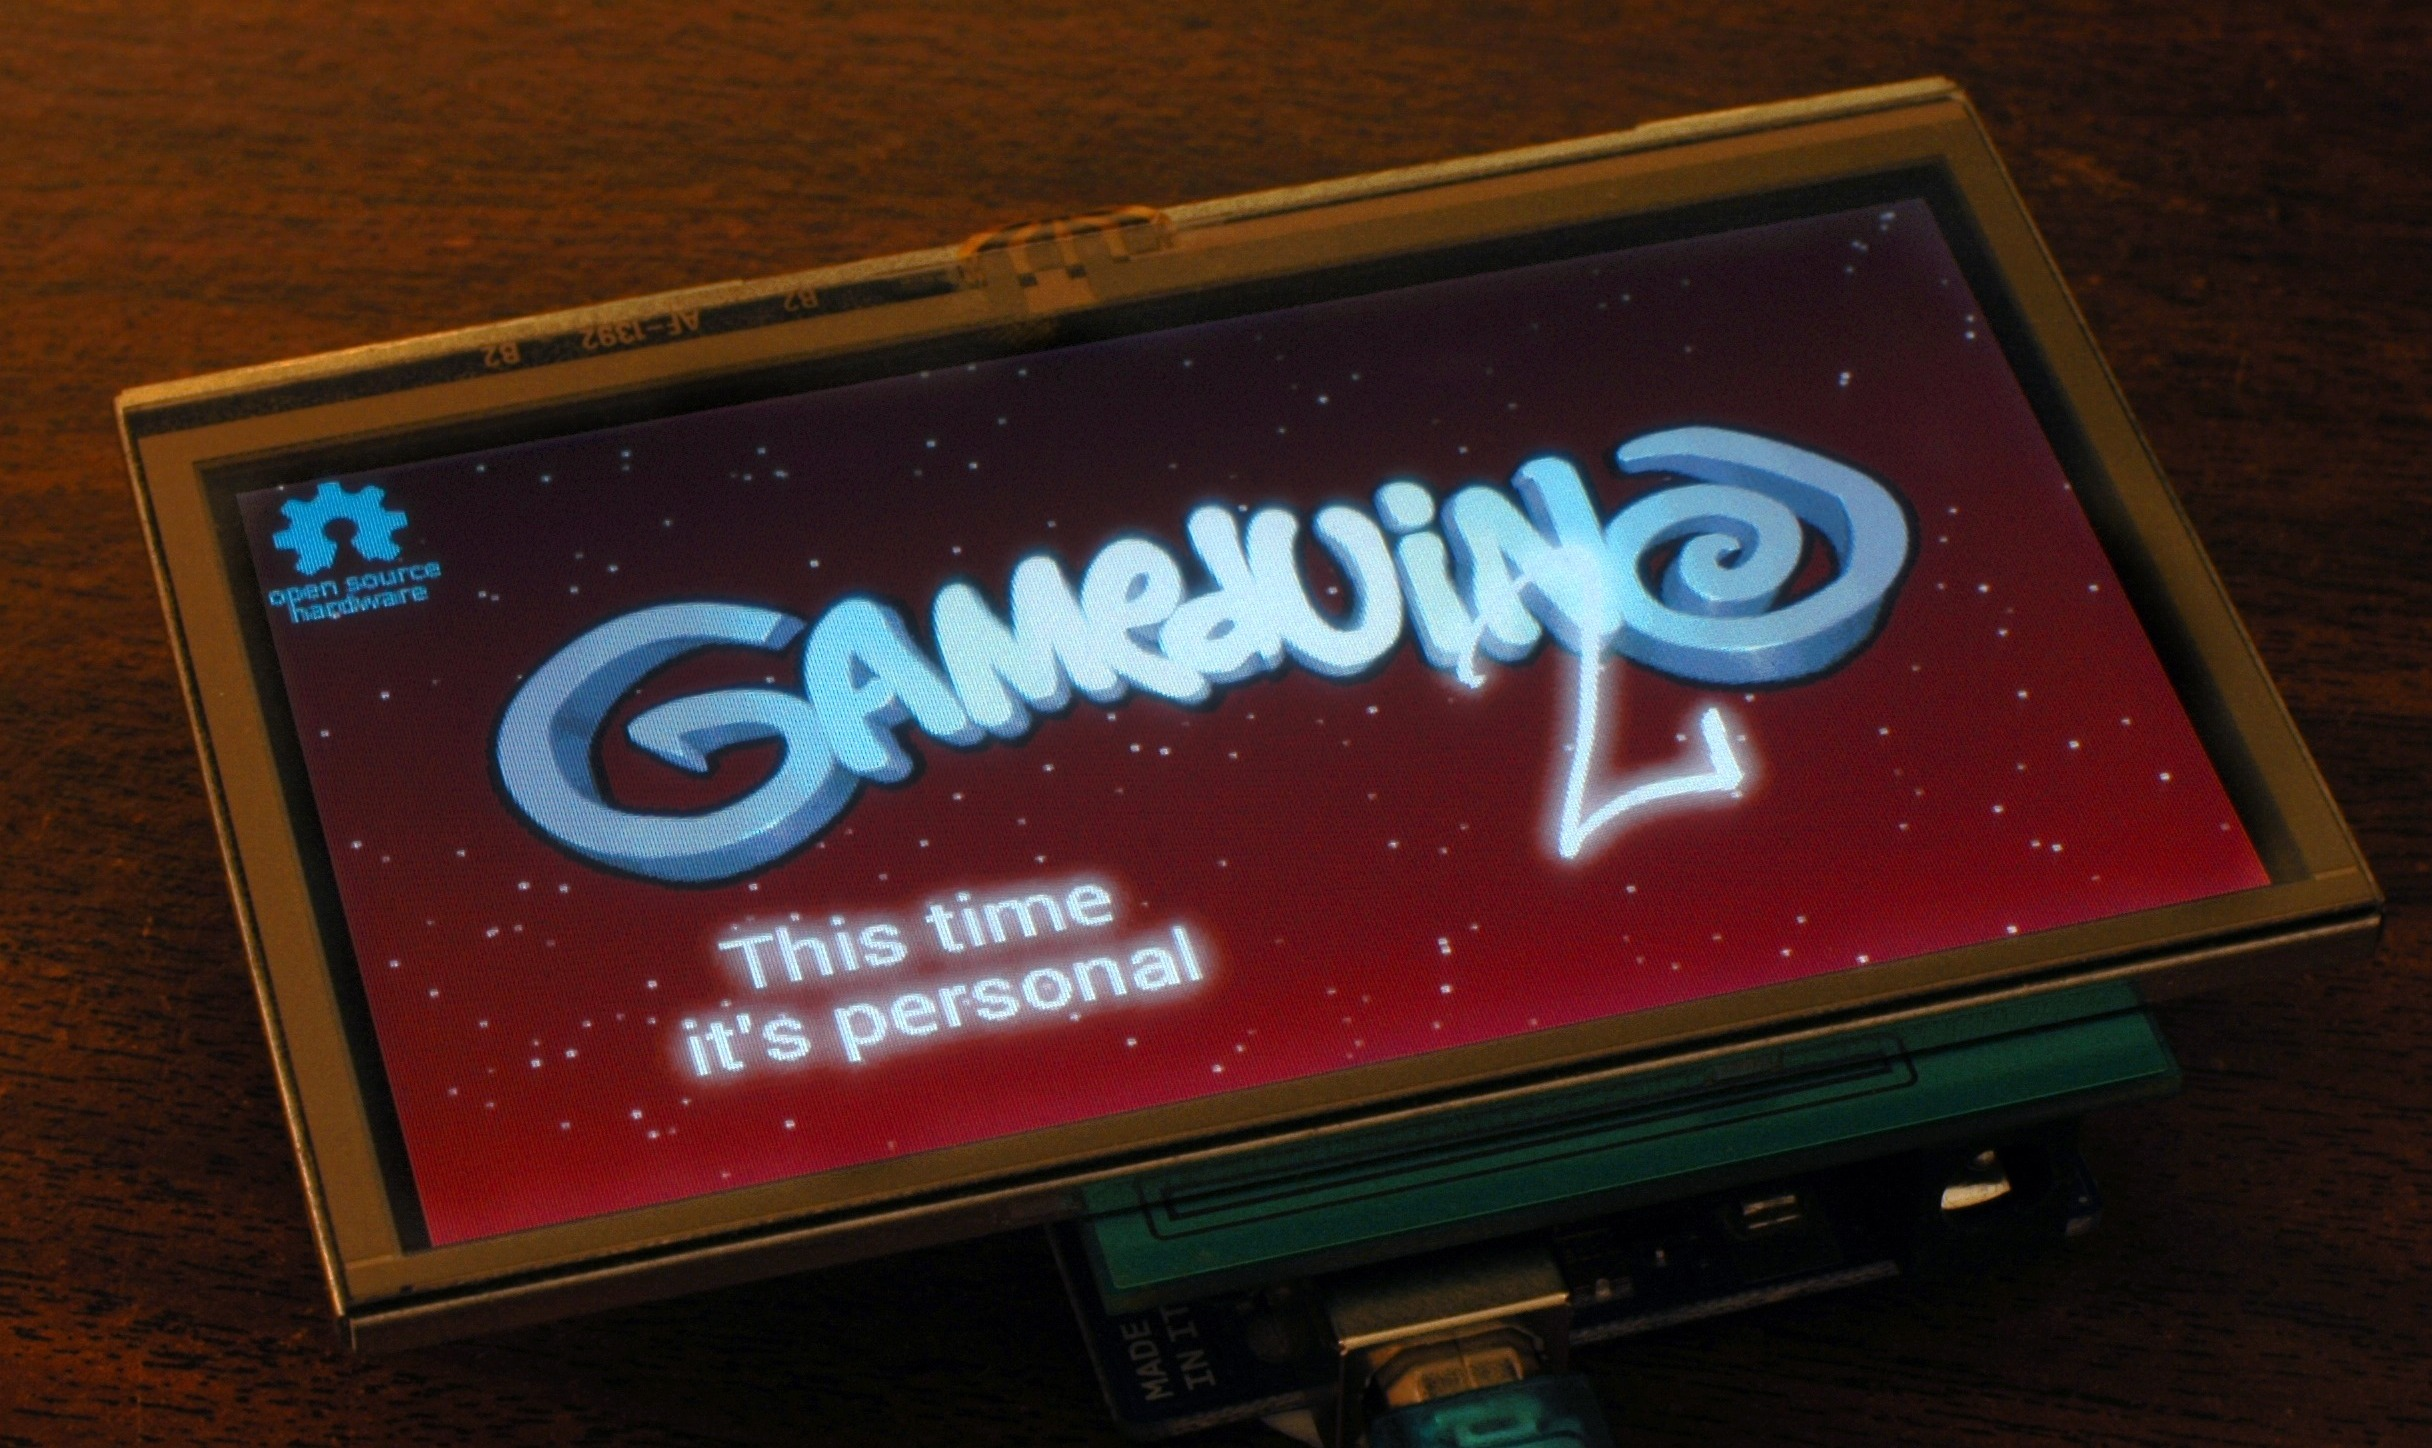
\includegraphics[width=0.9\textwidth]{assets/plugin.jpg}
\end{center}

\begin{enumerate}

\item
从 \url{http://gameduino.com/code} 下载 \gdtwo 的程序库 \mach{Gameduino2.zip} 并且将其安装至Arduino IDE中。
如果不知道如何安装Arduino第三方程序库,可以在 \url{http://arduino.cc/en/Guide/Libraries} 找到详细步骤。

\item
将 \gdtwo 连接至Arduino的插槽中,连接时确认所有的引脚都正确对齐。

\item
将Arduino插入电脑USB端口为其通电。因为当前还没有程序载入到Arduino中,此时 \gdtwo 的屏幕上不会有任何内容显示。

\item
启动Arduino IDE并且载入一个Gameduino 2的示例程序,如 \\
\begin{small}
\mach{File} $\triangleright$
\mach{Sketchbook} $\triangleright$
\mach{libraries} $\triangleright$
\mach{Gameduino2} $\triangleright$
\mach{1.Basics} $\triangleright$
\mach{helloworld}
\end{small}

\begin{center}
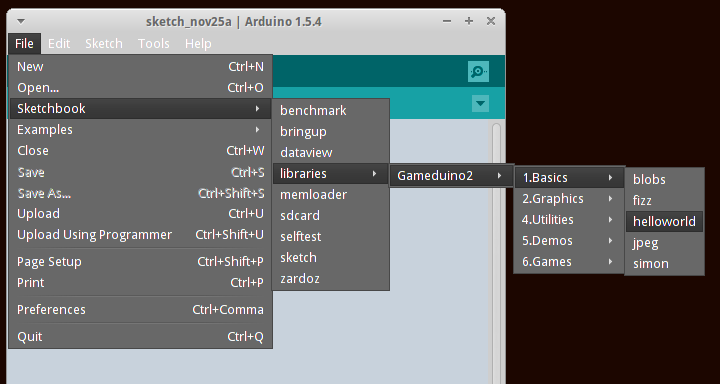
\includegraphics[width=1.0\textwidth]{assets/menu.png}
\end{center}

\item
点击下载按钮将程序编译并载入到Arduino中,等待一段时间后, \gdtwo 将会启动并开始绘制载入的程序。

\item
很多示例程序需要从microSD中读取数据。为了能正常运行这些程序,需要准备一张格式化后的microSD卡,并将 \mach{Gameduino2sd.zip} 压缩包中的文件拷入到SD卡中 (该文件可从 \url{http://gameduino.com/code} 上下载)。

\item
试着运行其他的例程,劲情享受!

\end{enumerate}

%%%%%%%%%%%%%%%%%%%%%%%%%%%%%%%%%%%%%%%%%%%%%%%%%%%%%%%%%%%%%%%%%%%%%%%%
\chapter{快速入门}

本章介绍了 \gdtwo 的基本编程方法\ - 从 ``hello world'' 到创建一个简单的触屏游戏。

\newcommand*\cleartoleftpage{%
  \clearpage
    \ifodd\value{page}\hbox{}\newpage\fi
    }

\cleartoleftpage
\section{Hello world}
\label{helloworld}
\index{drawing!text}
\index{text, drawing}
\index{demos!hello world}

\png{helloworld}

\newcommand{\eg}[1]{
\begin{framed}
\input{code/#1.inc}
\end{framed}
}

\eg{helloworld-A}

以上示例代码中,函数 \mach{loop()} 首先将屏幕背景设置为深绿色,之后将一段文字显示在屏幕的正中央。这个代码将以每秒钟 $60$ 次的速度连续执行,但由于每次写入的内容相同,屏幕上不会看出任何变化。

\dcmd{ClearColorRGB} 是一个绘图指令:它设置了屏幕清屏时所使用的背景色。
这里所用的颜色是深绿色 \texttt{0x103000}。 \gdtwo 和HTML一样,使用三个 $16$ 进制数来表示颜色。
\index{HTML color triplet}

\dcmd{Clear} 是另外一个绘图指令,它将屏幕清除为ClearColorRGB()中所设置的颜色。所有的绘图都是从清屏指令开始的。

\cmd{text} 是一个高级GPU绘图指令。该指令在屏幕指定位置用特定字体绘制字符串。在这个例子中,文字被绘制在屏幕的正中心, $(x,y)$ 坐标 $(240,136)$ 处。
\mach{OPT\_CENTER} 参数的作用是指明绘制文本时提供的坐标为中心坐标,所以文本绘制时的中心将被设置为 $(240,136)$。
参数中的 $31$ 是文本的字号,$31$ 是内置字体中能设置的最大字号。

最后 \mach{GD.swap()} 函数告知图形系统图形绘制已经完成,并将绘制完成后的图形内容显示到显示屏上。在Gameduino中有两份图像的拷贝,一份是在屏幕上实际显示出来的图形,一份是在缓存中用户正在编辑的图形。调用 \mach{GD.swap()} 函数将把缓存中的内容同步到屏幕上。
这种交换机制 (又称\term{双缓冲}) 可以使显示的内容更新时更加平滑,只有程序调用 \mach{GD.swap()} 时才会进行一次真正的绘制。

\index{screen coordinates}
\index{coordinates, screen}
\gdtwo 的屏幕分辨率为宽 $480$ 像素,高 $272$ 像素。
屏幕的左上角坐标是 $(0,0)$,屏幕的右下角坐标是 $(479,271)$,屏幕中心坐标点在 $(240,136)$。

\begin{center}
\begin{tikzpicture}
    [align=center,node distance=4cm]
    \node [opacity=0.2,inner sep=0] at (0,0) (png) {
\includegraphics[width=0.8\textwidth]{assets/helloworld.png}};

    \node [below of=png] (240x136) {$x=240,y=136$)};
    \draw [-latex]   (240x136) -- (png.center);

    \draw [-latex]   (png.north west) -- (png.north east)
      node[above left,pos=0] {$x=y=0$}
      node[above] {$x=480$};
    \draw [-latex]   (png.north west) -- (png.south west)
      node[left] {$y=272$};

\end{tikzpicture}
\end{center}

\newpage
\section{点与圆}
\index{points} \index{circles}
\defidx{POINTS}
\index{drawing!points}
\index{points}

那么如何使用 \gdtwo 绘制图形呢?图形绘制有两个指令:\dcmd{Begin} 和 \dcmd{Vertex2ii}。
其中 \dcmd{Begin} 告知图形系统将要绘制的图形类型,而 \dcmd{Vertex2ii} 将该图形在指定位置绘制出来。以下代码实现了在 $(220,100)$ 和 $(260,170)$ 两处分别绘制两个单位像素大小的坐标点:

\eg{examples-a}

\png{0000}

\mach{Begin(POINTS)} 函数告知GPU准备开始进行点绘制。之后的 \dcmd{Vertex2ii} 函数调用在指定的屏幕坐标 $(x,y)$ 处绘制一个新点。注意如果不先调用准备绘制函数 \dcmd{Begin}, 那么硬件无从得知将要绘制的图形类型,从而导致其忽略接下来所有的 \dcmd{Vertex2ii} 的调用。

\newpage
GD图形库还包含
\dcmd{PointSize} 调用,该函数用于设置绘制点的大小。此函数仅有一个参数:绘制点的直径,单位为 $1/16$ 像素。硬件系统使用子像素机制
(\term{subpixel}) 让用户对绘制物体的尺寸有更好的控制。子像素相比以像素作为单位,可以显著提高显示的精度和效果。
当你希望使用像素表示长度或直径的时候,最好在代码中显式将对应的数值乘以 $16$ 。

这里,在调用点绘制函数之前增加了一个 \dcmd{PointSize} 调用,绘制了一个半径为 $30$ 像素(即\term{直径} $60$ 像素)的圆点。

\png{0001}
\eg{examples-b}


实际上,硬件系统总是以和绘制圆相同的方式来绘制点( \mach{POINTS} )。但当绘制圆的半径很小时,此时绘制的圆看上去等效于一个像素点。
所以在Gameduino中,点与圆如同手足不可分割。

\newpage
\section{色彩与透明度}

在绘制vertex图形之前,还可以通过 \dcmd{ColorRGB} 函数改变绘制的颜色:

\png{0002}
\eg{examples-c}

\dcmd{ClearColorRGB}, \dcmd{ColorRGB} 和 \dcmd{PointSize} 都属于设置\term{图形状态}的功能函数,
这些图形状态好比是图形硬件系统中的变量一样。当这些状态被程序更改之后,将会影响到之后的绘图操作。为了让生活美好一点,所有的图形状态在每一帧的开始处被恢复成了默认值。你可能想到了,对于 \dcmd{ColorRGB} 来说,默认的颜色就是是白色的,这也是为什么之前的 ``Hello world'' 会是白色的。而默认的 \dcmd{PointSize} 是 $8$ ,也就是半个像素的直径大小。

你也可以如同改变颜色一样自如的改变绘图的透明度。透明度是通过 alpha 通道控制的,有效设置范围为 $0\sim255$。
\index{alpha}
\index{transparency, alpha}
其中 $0$ 表示完全透明,而默认值 $255$ 表示完全不透明。以下是利用 \dcmd{ColorA} 函数将透明度设置为 $128$,也就是 $50\%$ 的透明度,得到的效果:

\png{0003}
\eg{examples-d}

颜色修改函数 \dcmd{ColorRGB} 和 \dcmd{ClearColorRGB} 同样接受 (R, G, B) 分立值作为参数。
所以 \mach{ColorRGB(0x0080ff)} 也可以写为 \mach{ColorRGB(0, 128, 255)}:

\eg{examples-triplet}

\newpage
\section{设计示例: fizz}
\label{fizz}
\index{demos!fizz}

\png{fizz}
\eg{fizz-a}

``fizz'' 程序在每一帧中绘制 $100$ 个圆,每一个圆都具有随机的大小、颜色和透明度。
虽然每一帧的执行时间仅有 $1/60$ 秒,但因为人眼存在视觉暂留,一眼看上去就好像无数五彩斑斓的圆盘一样。
\index{frenzy, seething}

\begin{center}

\includegraphics[width=0.24\textwidth]{assets/fizz-6.png}

\includegraphics[width=0.24\textwidth]{assets/fizz-7.png}

\includegraphics[width=0.24\textwidth]{assets/fizz-8.png}

\includegraphics[width=0.24\textwidth]{assets/fizz-9.png}
\end{center}


\section{播放音符}

\gdtwo 有两种方式播放声音,一种是使用内置的音频采样文件,一种是播放用户自己的采样文件。
对于前者,只要调用 \mach{GD.play()} 函数,并指明使用的乐器及MIDI音符编号就可以播放对应音符:
\index{MIDI notes}

\eg{examples-e}

\defidx{HARP}\defidx{XYLOPHONE}\defidx{TUBA}\defidx{GLOCKENSPIEL}\defidx{ORGAN}\defidx{TRUMPET}\defidx{PIANO}\defidx{CHIMES}\defidx{MUSICBOX}\defidx{BELL}
\mach{GD.play()} 函数是非阻塞执行的:即使之前的音乐没有播放完,下一个音乐也会立刻开始播放。为了防止这种情况的出现,这里调用了
\mach{delay()} 延时1秒来等待之前的音符播放完毕。\gdtwo 可用的内建乐器列表如下:
\index{instruments}
\mach{HARP},
\mach{XYLOPHONE},
\mach{TUBA},
\mach{GLOCKENSPIEL},
\mach{ORGAN},
\mach{TRUMPET},
\mach{PIANO},
\mach{CHIMES},
\mach{MUSICBOX} 和
\mach{BELL}。
虽然这些内置采样的音质并不高
\footnote{其中\mach{PIANO} 可能是最糟糕的了,其次是\mach{TUBA} :听起来都不像一个常规的乐器。
}
,但这里只是将它们作为简易手段来测试音频功能。
确定了播放乐器之后,还需要确定MIDI编号。在 \gdtwo 中,每个乐器可以播放的MIDI编号范围是 $21\sim108$。

还有一些可以连续播放的声音:
\index{wave instruments}
\mach{SQUAREWAVE},
\mach{SINEWAVE},
\mach{SAWTOOTH} 和
\mach{TRIANGLE}。
这些声音特别适合用于创造独特的声音效果,产生复古的音效感。不同于之前的乐器音效,这些声音如果不主动中断,将会无限期地播放下去。
除了这些乐器音效以外,这里还有一小部分打击乐的采样音效。这些音效不使用MIDI编号参数,所以在程序编写时直接忽略,如 \mach{GD.play(NOTCH)}。
这部分可用的音效列表如下:

\vspace{10pt}
\begin{tabular}{l}
\mach{CLICK} \\
\mach{SWITCH} \\
\mach{COWBELL} \\
\mach{NOTCH} \\
\mach{HIHAT} \\
\mach{KICKDRUM} \\
\mach{POP} \\
\mach{CLACK} \\
\mach{CHACK} \\
\end{tabular}
\vspace{10pt}
\defidx{CLICK} \defidx{SWITCH} \defidx{COWBELL} \defidx{NOTCH} \defidx{HIHAT} \defidx{KICKDRUM} \defidx{POP} \defidx{CLACK} \defidx{CHACK}

注意负责音频播放的硬件同时只能播放一个音效,播放任何其他的声音都将中断上一个声音的播放。

\defidx{SILENCE}
如果需要主动停止声音播放,可以使用函数 \mach{GD.play(SILENCE)}。

\newpage
\section{触摸标签}

屏幕上的每个可见像素除了有对应的颜色之外,还有一个不可见的触摸标签值。这个标签值用来判断触摸发生的位置。
以下代码演示了如何将两个彩色圆盘的标签值分别设置成为 $100$ 和 $101$:

\eg{examples-f}

\noindent
这个代码会生成和之前一样的图形:

\png{0002}

但是这个程序不同之处在于,一旦系统检测到在这两个圆上发生了触摸动作,就会将对应的标签值(这里是 $100$ 或 $101$)记录保存下来。之后再使用一个循环结构不断读取当前的触摸标签值 ( \nameref{getinputs} 函数会将最新的触摸标签值更新至 \mach{GD.inputs} ),并将其输出到屏幕上:

\eg{examples-g}

这样一来,每当你按下其中一个圆盘的时候,从串口输出中就会返回 $100$ 或 $101$ 的代码。触摸标签机制提供了一种非常实用的交互方法,如果没有这个功能,那么代码必须检测每一次触摸的 $(x,y)$ 坐标,并依次判断该坐标是否落在对应的按钮半径范围内。而通过使用触摸标签,代码为每个对象分配一个 \dcmd{Tag} 作为标签值,随后硬件自动进行像素判断并记录触摸对象的标签值。为了实现这个功能,设备还需要持续追踪每个像素的 \dcmd{Tag} 值。这被称为``标签缓存''——下面是标签缓存的一个例子:

\vspace{10pt}

\begin{tikzpicture}
  \node[anchor=south west,inner sep=0,opacity=0.2] (image) at (0,0) {
\includegraphics[width=0.9\textwidth]{assets/0002.png}};
  \begin{scope}[x={(image.south east)},y={(image.north west)},xscale=0.20833333333333334,yshift=0.51\textwidth,yscale=-0.3676470588235294]
    \draw[black, ultra thick] (2.20,1.00) circle (0.30);
    \draw[black, ultra thick] (2.60,1.70) circle (0.30);
    \draw[black, thick] (0,0) rectangle (4.80,2.71);
    \node at (2.20,1.00) {100};
    \node at (2.60,1.70) {101};
  \end{scope}
\end{tikzpicture}

\vspace{10pt}

\noindent
每当屏幕被点击,设备都将查找标签缓存中对应像素标签值,并将其记录在 \mach{GD.inputs.tag} 中。

\cleartoleftpage
\section{游戏设计: Simon}
\label{simon}

\png{simon}

这是一个诞生于 $1978$ 年的记忆游戏``Simon''。 这个游戏的规则是:系统按照随机顺序点亮屏幕中的四个指示灯之一,而玩家必须按照正确的顺序重复出来。
如果你全部答对,系统就会在原序列中再额外增加一个步骤,如此重复直到你出现失误为止。

以下代码首先定义了游戏中使用到的主要颜色,之后将利用这些颜色绘制游戏界面:

\eg{simon-a}

\noindent

游戏的主界面是四个大圆盘,每一个对应一个按钮。按钮的颜色根据 \mach{pressed} 参数决定是否要高亮显示。
在绘制按钮之前调用了 \dcmd{Tag} 函数设置标签缓冲,这样在该按钮的任意位置点击都会在 \mach{GD.inputs.tag} 中返回对应数值。

\newpage
\eg{simon-b}

函数 \mach{play()} 根据被点击的按钮播放不同的音效,同时点亮相应的圆盘半秒(即 $30$ 帧)。

\eg{simon-play}

\mach{get\_note()} 是一个用户输入程序。
它的作用是绘制游戏界面,同时每次绘制都将查看 \mach{GD.input.tag} 以确定是否有按钮被点击。
一旦有按钮被点击,它将调用 \mach{play()} 来播放音效与处理高亮,最后返回按钮的对应数值。

\eg{simon-getnote}

\mach{loop()} 函数实现了完整的游戏循环过程。
程序每次都将在原按钮序列后添加一个新的随机按钮,演示这一新序列,并要求玩家按顺序重复按钮序列。
如果玩家重复点击的顺序完全正确,游戏会一直继续下去;
如果玩家的点击出现任何错误,游戏将发出表示''失败''的音效并退出,随后下一次 \mach{loop()} 函数将重新启动游戏。

\eg{simon-loop}

%%%%%%%%%%%%%%%%%%%%%%%%%%%%%%%%%%%%%%%%%%%%%%%%%%%%%%%%%%%%%%%%%%%%%%%%
\chapter{位图}

\gdtwo 的GPU模块对绘制位图有硬件级别的支持,\gdtwo 中支持的位图种类有:

\begin{itemize}
\item 任意尺寸,从 $1 \times 1$ 像素到 $512 \times 512$
\item 可在其他位图图像上进行重复叠加
\item 重新着色并在绘制时增加透明度
\item 在x和y轴方向进行无限重复绘制(又称 \term{tiling})
\item 旋转,拉伸和收缩
\end{itemize}

位图图像的数据——代表位图各像素点信息的字节数据——存储在GPU的主存储器中。这一主存储器的大小是 $256$ KB。

从某种程度上说,位图是过去游戏机硬件所使用的图元(\term{sprites})的传承。在一些代码中仍可看到 \textit{sprite} 这个词 
——它通常只是表示在到处移动的位图。

\newpage
\section{载入一张JPEG}
\index{jpeg}

\png{jpeg}

\eg{jpeg-A}

以上代码中,\cmd{loadimage} 的作用是通知GPU将会有一张JPEG载入到内存地址 \mach{0} 处。 
\nameref{load} 从microSD卡中读取文件 \mach{healsky3.jpg}\footnote{Artwork by J. W. Bjerk (eleazzaar) -- www.jwbjerk.com/art} 并直接将其提供给GPU,GPU将它作为一张位图存储到显存中。 
\dcmd{Begin} 调用使用 \mach{BITMAPS} 参数,这样随后每次调用 \dcmd{Vertex2ii} 都将以给定的坐标 $(x,y)$ 作为左上顶角来绘制载入的图像。

\section{位图尺寸}

之前我们知道了每次调用 \dcmd{Vertex2ii} 都会绘制一幅位图,例如这段代码

\eg{examples-i}

将会生成下图:

\png{0006}

原始JPEG文件的尺寸为 $128 \times 128$ ,因此每次调用 \dcmd{Vertex2ii} 
都将在大小为 $128 \times 128$ 的像素区域中绘制这一位图图像。
不过你可以通过 \dcmd{BitmapSize} 来调节绘制位图的区域尺寸。
例如:

\eg{examples-j}

改变位图绘制尺寸后,只有 $64 \times 64$ 的区域被绘制出来:

\png{0007}

如果我们增大位图绘制区域到比原图更大的尺寸,如 $480 \times 272$:

\eg{examples-k}

却并没有得到比原图 $128 \times 128$ 更大的尺寸:

\png{0008}

为什么会这样呢? 其实,GPU的确绘制了一幅 $480 \times 272$ 尺寸的图像,
但是因为原图的尺寸只有 $128 \times 128$ ,多余的空间就会被用透明的黑色像素填满。
但如果将参数 \mach{BORDER} 改为 \mach{REPEAT} ,GPU就会在绘制区域内的x和y轴方向上无限地重复绘制原图像。

\index{bitmaps!tiling}

\eg{examples-l}


\png{0009}
\clearpage

\section{位图句柄}
\label{bitmaphandles}

\png{jpeg2}

\eg{jpeg2-A}

以上这段代码的功能是在显存中存放了两张JPEG图片——其中一张日出图片存放在了在地址 \mach{0} 处,还有一张名为 \mach{healsky3} 的图片。值得注意的是,其中第二个 \mach{load\_image()} 的调用中将 \mach{$-1$} 作为地址参数,这一特殊数值的含义是告知载入程序将这张JPEG图片紧跟在当前显存的最后一张图片之后。
通过这种方式可以很方便的存储一连串图片,而无需计算每张图片的具体存储位置。

通过在将图片载入前设定相应的位图句柄,设备能够时刻追踪到这两张图片的各项参数——大小、格式、存储地址——
而在绘图代码中也可以通过这两个句柄对这两张图片进行选择。

在绘制位图( \mach{BITMAPS} )时,\dcmd{Vertex2ii} 还有第 $3$ 个参数。
这个参数用于指定绘制位图的相应句柄,其缺省值为 $0$ 。
以下代码在位图句柄 $0$ 和 $1$ 中随机选择,并连续绘制了 $100$ 张位图。最终的结果呈现出一幅随机混杂的图像,视觉上和 \nameref{fizz} 相似。
\eg{examples-m}
\png{0010}

硬件系统提供 $16$ 个可用的位图句柄供用户使用,其有效范围是 $0\sim15$。
用户可以在绘制过程中重新分配位图句柄,因而可供应用程序使用的位图不局限于 $16$ 张。
事实上,大部分应用程序不会用到 $16$ 张以上的图片,因此各图片通常在 \mach{setup()} 中就分配好对应的句柄。

\newpage
\section{位图的像素格式}
\index{bitmaps!formats}

在理想情况下,所有位图的色彩都应该实现百分之百的还原。不过受限于GPU和Arduino的内存,用户只能在色彩还原度和存储空间上寻找一个平衡点。对此,Gameduino 2 提供了多种可供使用的图片格式:
\\
\newcommand{\fmline}[3]{
\index{#1 bitmap format@\mach{#1} bitmap format}
\index{bitmap format!#1@\mach{#1}}
\textbf{\large\mach{#1}} &
#3
& {\raisebox{-96pt}{\includegraphics[height=100pt]{#2}}} \\
}

\noindent
\begin{tabular}{p{0.15\textwidth}p{0.35\textwidth}p{0.4\textwidth}}
\fmline{L8}{previews/formats-PHOTO_L8-00.png}{
每像素 $8$ 位数据,最高质量的单色图片格式。
} \\
\fmline{L4}{previews/formats-PHOTO_L4-00.png}{
每像素 $4$ 位数据,适用于单色图标或字体。} \\
\fmline{L1}{previews/formats-PHOTO_L1-00.png}{
每像素 $1$ 位数据,用于实现复古的图形风格;同样也适用于分层和蒙版效果。} \\
\end{tabular}
\newpage

\noindent
\begin{tabular}{p{0.15\textwidth}p{0.35\textwidth}p{0.4\textwidth}}
\fmline{RGB565}{previews/formats-PHOTO_RGB565-00.png}{
每像素 $16$ 位数据:其中各有 $5$ 位用于存储红色和蓝色信息,$6$ 位用于绿色信息。
适用于大多数没有透明度设置的照片或图片。
} \\
\fmline{ARGB1555}{previews/formats-PHOTO_ARGB1555-00.png}{
每像素 $16$ 位数据:其中各有 $5$ 位用于存储红色、绿色和蓝色信息,另有 $1$ 位记录透明度信息。
这个仅有 $1$ 位的透明度通道只可实现简单的开启或关闭设置。
% This was the sole color format of the orginal Gameduino.
} \\
\fmline{ARGB4}{previews/formats-PHOTO_ARGB4-00.png}{
每像素 $16$ 位数据:各有 $4$ 位用于存储红色、绿色、蓝色和透明度信息。
适用于存储需要有光滑透明边缘的图片,例如:彩色图标和图元。} \\
\fmline{RGB332}{previews/formats-PHOTO_RGB332-00.png}{
各有 $2$ 位用于存储红色和蓝色信息,$3$ 位用于绿色信息。有时也用于图像显示和图标。} \\
\fmline{ARGB2}{previews/formats-PHOTO_ARGB2-00.png}{
各有 $2$ 位用于存储红色、绿色、蓝色和透明度信息,不太适用于图片的显示,但可用于复古风格的图元或者色彩度较低的图标中。} \\
\end{tabular}
\newpage

\section{位图着色}

\png{0011}

和其它绘图指令一样, \mach{BITMAPS} 也存在当前颜色的设定。该颜色会与原图像的颜色混合,呈现出一种透过彩色玻璃看它的感觉。

\eg{examples-n}

如果当前 RGB 颜色设定为白色(\mach{0xffffff}),则原图像色彩保持不变。而如果将颜色设定为黑色(\mach{0x000000}),则原图像的所有像素都将被填涂为黑色。
\clearpage

\newpage
\section{转化图形}
\index{asset converter}
\label{assets}

将一个图片资源转换为 \gdtwo 可用的位图格式的步骤并不简单。对此, \gdtwo 的内置工具中包含一个资源转换器(asset converter),该工具可以读取图片源文件并将其转换为 \gdtwo 可用的位图格式。


资源转换器的输出为一个名为 \mach{x\_assets.h} 的头文件,其中 \mach{x} 是用户转换图片的文件名。在这个头文件中,定义了一个宏函数 \mach{LOAD\_ASSETS()},它的作用是将转换后的图片载入到 \gdtwo 的显存中。该文件的使用方法是:首先在程序开头包含这个头文件,然后在调用 \mach{GD.begin()} 后,调用函数 \mach{LOAD\_ASSETS()}:

\eg{walk-load}

在 \mach{LOAD\_ASSETS()} 完成后,所有的位图都将加载到显存中,并且位图句柄也将设定完毕以便用其实现位图操作。
这些位图句柄同样在头文件中说明,之后的代码可以直接使用这些句柄,如下所示:

\eg{walk-asset}

使用资源转换器和之前直接从JPEG文件中载入图片相比有两个优点:

第一,JPEG图片只能被加载为 \mach{RGB565} 格式的位图,这是因为在JPEG图片中没有透明度信息,所以这是唯一支持的格式;

第二,资源转换器对图片进行无损( \textit{losslessly} )压缩 \footnote{
压缩方案为 zlib INFLATE
( \url{http://www.zlib.net/} ),即gzip和Zip所使用的压缩方案。
GPU为zlib INFLATE提供硬件支持。} ,而JPEG使用的是有损压缩。
对于一般的摄影图像差别虽然不大,但是对于精细绘制的游戏插图、图标和字体而言,有损和无损压缩的差别是相当明显的。

\newpage
\section{位图单元}
\index{sprites}
\index{bitmaps!animating}

\begin{center}

\includegraphics[width=0.11\textwidth]{previews/walk-WALK-00.png}

\includegraphics[width=0.11\textwidth]{previews/walk-WALK-01.png}

\includegraphics[width=0.11\textwidth]{previews/walk-WALK-02.png}
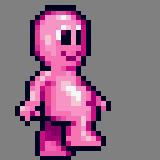
\includegraphics[width=0.11\textwidth]{previews/walk-WALK-03.png}

\includegraphics[width=0.11\textwidth]{previews/walk-WALK-04.png}
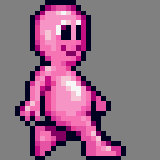
\includegraphics[width=0.11\textwidth]{previews/walk-WALK-05.png}

\includegraphics[width=0.11\textwidth]{previews/walk-WALK-06.png}

\includegraphics[width=0.11\textwidth]{previews/walk-WALK-07.png}
\end{center}

这 $8$ 张 $32 \times 32$ \mach{ARGB1555} 格式的位图图片循环构成一组走路的动画。
由于所有图片都采用乐同样的尺寸和格式,他们可以共用同一个位图句柄。
绘制命令会对具体绘制哪一个位图单元( \term{cell} )进行选择,这是在调用 \dcmd{Vertex2ii} 绘制位图时的第 $4$ 个参数。
下面这段代码演示了如何在屏幕上顺序显示这 $8$ 张动画图片:
\eg{examples-cell}
\noindent

\noindent
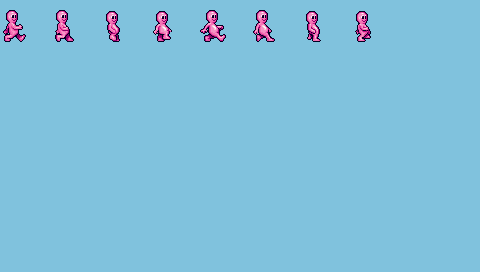
\includegraphics[width=\textwidth,trim=0 216 80 0,clip=true]{assets/0058.png}

每个位图句柄最多能够控制 $128$ 张位图单元,而这些位图单元在显存中是连续存放的。
位图单元对于显示动画是十分实用的,用户只需将动画每一帧的图片按顺序存储为一个位图句柄控制的位图单元,
就可以通过改变位图单元编号来控制相应的动画显示。

使用这 $8$ 帧动画序列,例程 \textit{walk} 在屏幕上创建了 $256$ 个走路的循环动画。
\index{demos!walk}
每组动画都有对应的计数器来控制它的 $x$ 坐标以及对应动画的帧编号。另外,动画图片所用的颜色从屏幕顶端的黑色( \mach{0x000000} )逐渐变化成屏幕底端的白色,从而产生了不同远近距离的效果。

\newpage
\png{walk}
\eg{walk-A}

% \newpage
% \section{Game: Fruit flicker 2000}
% \section{Zoom and shrink}

\newpage
\section{旋转,拉伸和收缩}
\index{rotation}
\index{zoom}
\index{bitmaps!rotating}
\index{bitmaps!zooming}
\png{0043}
\eg{examples-rot1}

位图的旋转和拉伸是由位图变换矩阵(\term{bitmap transform matrix})所控制的。这一矩阵属于图像属性的一部分,它控制着位图像素在屏幕上的映射方式。
值得欣慰的是,变换矩阵的数学计算大部分由设备硬件处理,因此用户可以轻松的实现像旋转和缩放这样的高级操作。

\newpage

由于 \cmd{rotate} 会累加操作,所以上例中将一幅位图分别以顺时针旋转 $0^\circ$、
$22.5^\circ$ 和 $45^\circ$ 绘制了 $3$ 次。
可以注意到这里图像只显示了一部分,这是因为旋转指令是以图片的左上角为中心进行旋转的。为了更好地观察这一现象,以下使用 \mach{(SRC\_ALPHA, ZERO)} 参数调用 \dcmd{BlendFunc} 函数将透明度设置取消:
\png{0044}

\noindent
\dcmd{Vertex2ii} 每次绘制 $128 \times 128$ 像素的图像,也就是所绘制图片的尺寸。
由于位图绘制是由变换矩阵决定的,当变换矩阵应用旋转变换后,图片也将随之旋转。

旋转发生的中心是位图图像的左上角,即例中图像 $(0, 0)$ 的坐标位置。
但一般对于旋转操作来说,通常将图片中心作为旋转中心,即例中图像 $(64, 64)$ 的坐标位置。
这个效果要分以下步骤实现:
\begin{enumerate}
\item 对图像进行平移变换( \textit{translate} ),使原坐标 $(64, 64)$ 移至 $(0, 0)$ 处;
\item 调用 \cmd{rotate} ,以当前 $(0, 0)$ 为中心旋转图像;
\item 对图像进行平移变换回原位置,即将现坐标 $(0, 0)$ 移回 $(64, 64)$ 处。
\end{enumerate}


\noindent
下面这个函数 \mach{rotate\_64\_64} 演示了上述三个步骤:

\samepage{
\eg{examples-rota}
}
上例调用 \cmd{translate} 命令使图像在 $x$ 和 $y$ 方向上各平移了 $64$ 像素。
\cmd{translate} 使用 $16.16$ 定点浮点数作为其参数,\mach{F16()} 宏函数将整数像素值转换为子像素坐标。
\png{0045}
\eg{examples-rot3}

\newpage
\cmd{scale} 指令可以用来缩放图像,通过增减比例实现拉伸或收缩图像。
下面例子中 \mach{scale\_64\_64()} 函数以图像 $(64, 64)$ 像素位置作为中心对图像进行缩放。
其中第一张图片是没有缩放的原图片;
第二张图片以 $2.0$ 作为缩放因子,将图片尺寸放大到两倍;
第三张图片以 $0.4$ 作为缩放因子,对图片进行收缩。

\png{0062}

\eg{examples-scale1}

%%%%%%%%%%%%%%%%%%%%%%%%%%%%%%%%%%%%%%%%%%%%%%%%%%%%%%%%%%%%%%%%%%%%%%%%
\chapter{更多的图形元素}
\newpage
\section{直线}
\defidx{LINES}
\index{drawing!lines}
\index{lines}
\label{lines}

\png{lines}

绘制直线的功能可以通过 \mach{Begin(LINES)} 或者 \mach{Begin(LINE\_STRIP)}函数实现。
\mach{LINES} 只成对连接端点绘制线段,而 \mach{LINE\_STRIP} 将所有端点按顺序首尾相接绘制线条。

\eg{lines-a}

游戏NightStrike使用 \mach{LINES} 绘制爆炸时``火花四溅''的效果。
\index{NightStrike}
每个火花都是一个包含当前位置 \mach{(x,y)}、速度 \mach{(xv,yv)} 和生命周期的对象。
当爆炸发生时,每一个火花以爆炸中心作为起始位置,并被赋予一个随机速度 \mach{(xv,yv)}。
而后每一个火花都会沿着自己的速度方向发散,绘制代码如下所示:

\eg{nightstrike-sparks}

这段代码绘制了一条以火花当前位置坐标点 $(x, y)$ 和下一位置坐标点作为两端的线段。
火花的大小(\dcmd{LineWidth})使用正弦公式计算得出,其开始时会由细变粗,之后再由粗变细直到彻底消失。
\index{sinusoidal}
\index{explosion}

\begin{center}
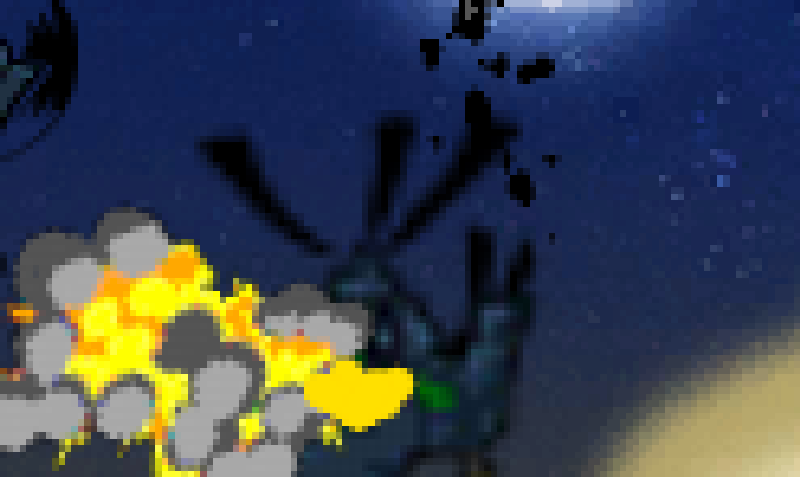
\includegraphics[width=0.3\textwidth]{assets/ns-lines-0000.png}
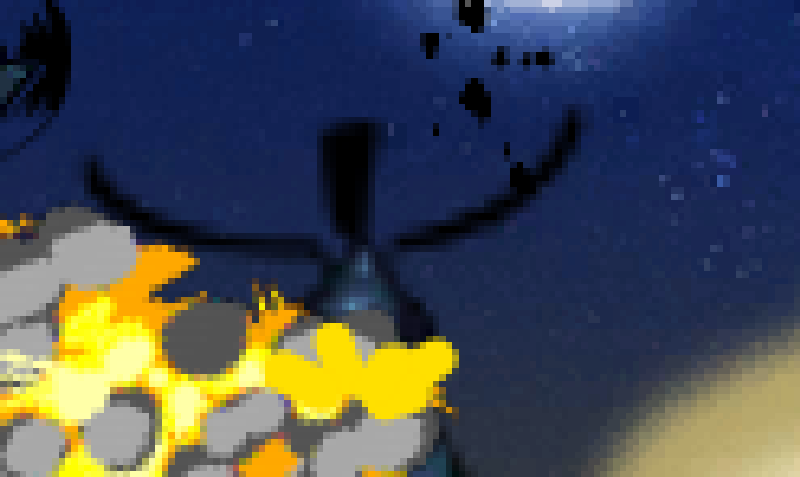
\includegraphics[width=0.3\textwidth]{assets/ns-lines-0001.png}
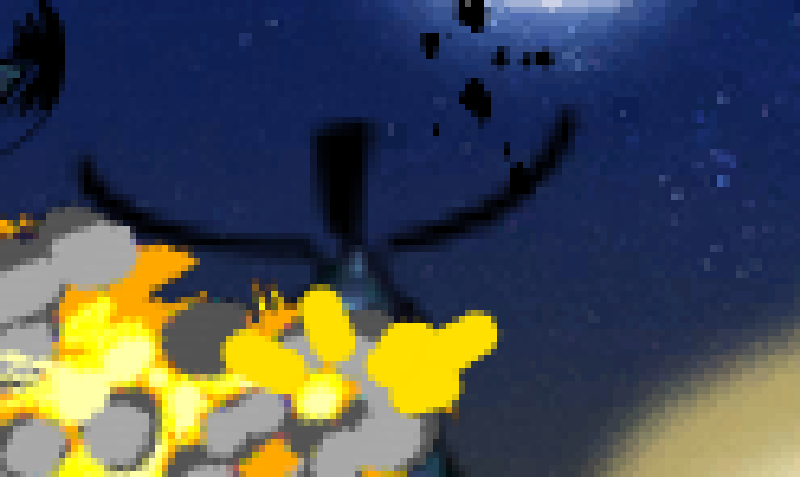
\includegraphics[width=0.3\textwidth]{assets/ns-lines-0002.png}
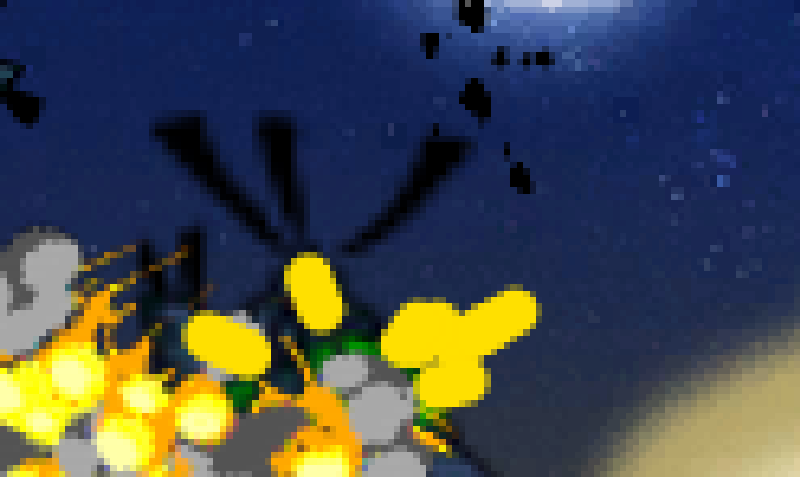
\includegraphics[width=0.3\textwidth]{assets/ns-lines-0003.png}
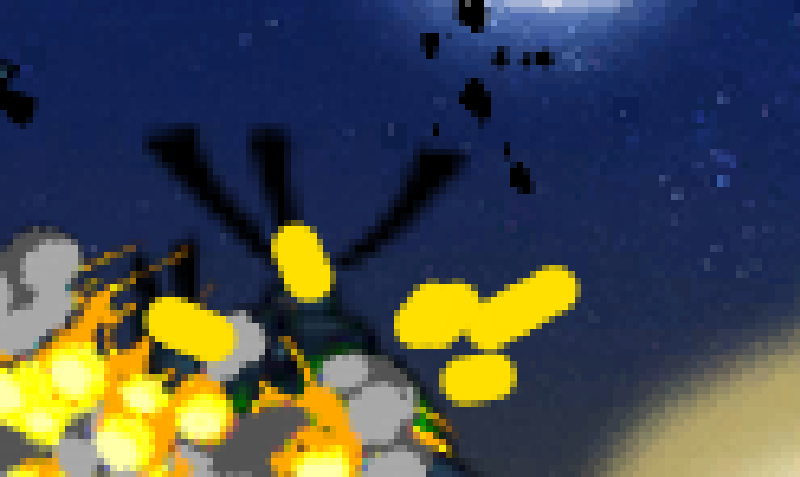
\includegraphics[width=0.3\textwidth]{assets/ns-lines-0004.png}
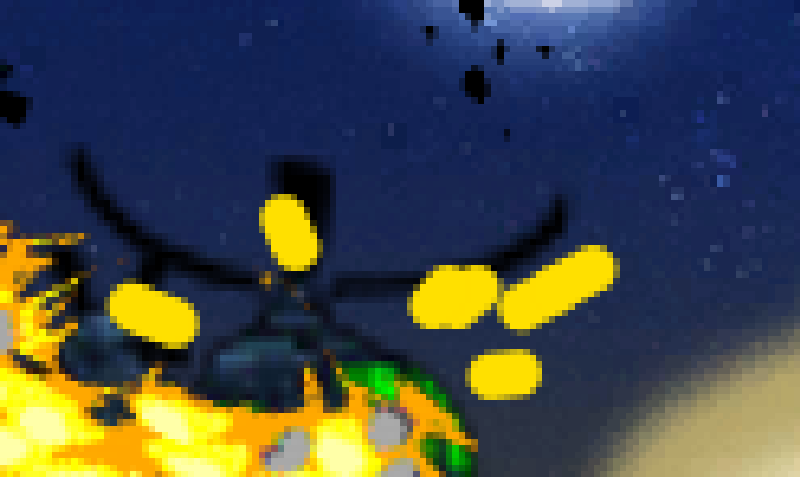
\includegraphics[width=0.3\textwidth]{assets/ns-lines-0005.png}
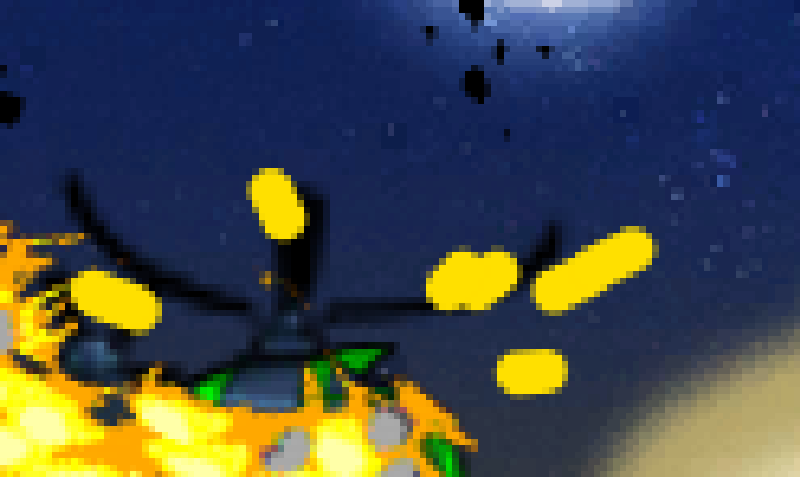
\includegraphics[width=0.3\textwidth]{assets/ns-lines-0006.png}
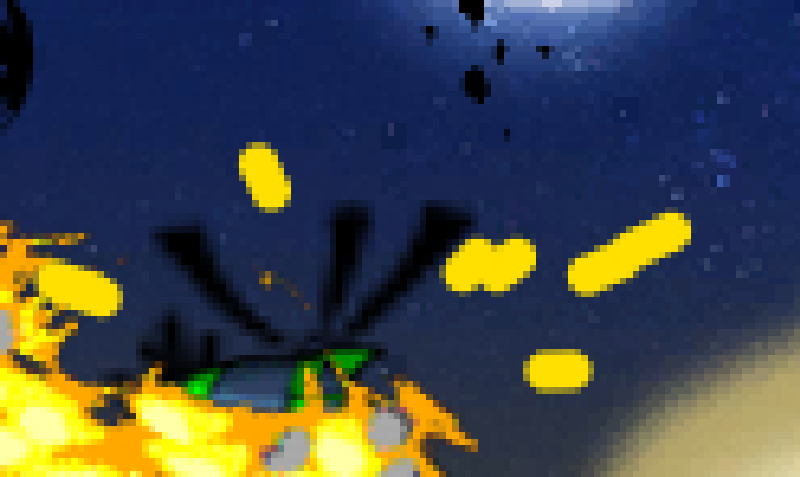
\includegraphics[width=0.3\textwidth]{assets/ns-lines-0007.png}
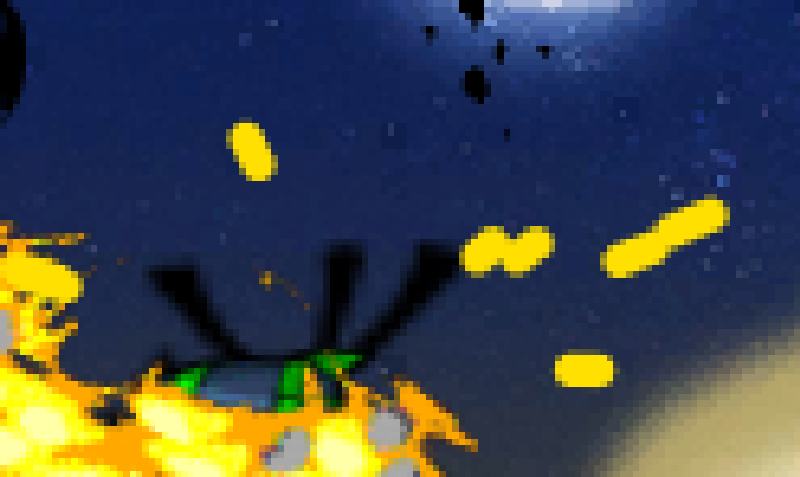
\includegraphics[width=0.3\textwidth]{assets/ns-lines-0008.png}
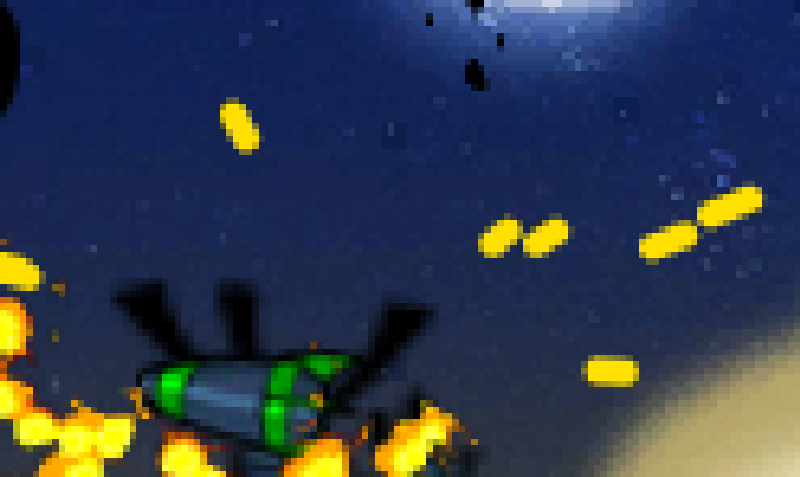
\includegraphics[width=0.3\textwidth]{assets/ns-lines-0009.png}
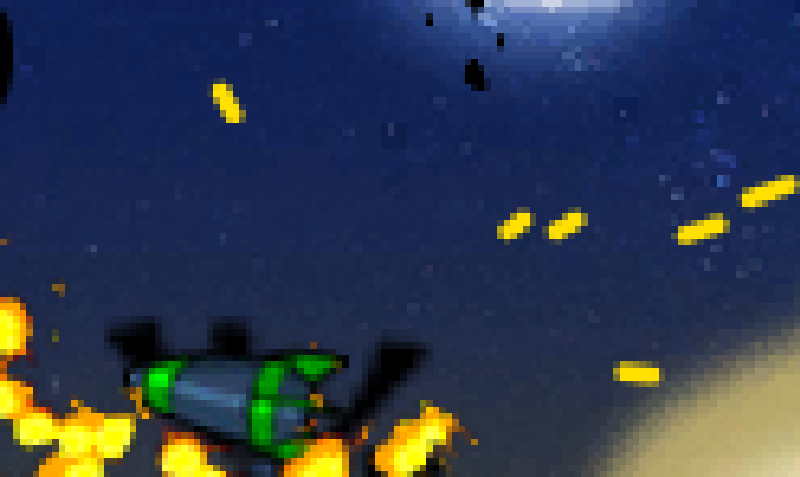
\includegraphics[width=0.3\textwidth]{assets/ns-lines-0010.png}
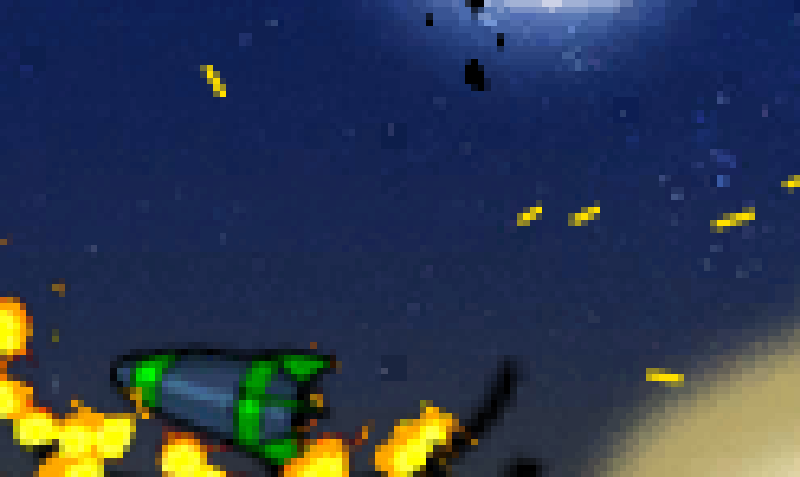
\includegraphics[width=0.3\textwidth]{assets/ns-lines-0011.png}
\end{center}

以上连续 $12$ 帧的图片展现了一个火花四射的完整过程,因为游戏运行帧数为 $60$ fps,所以每个火花的生命周期大约是 $0.2$ 秒。
\index{sparks}

\newpage
\section{矩形}
\defidx{RECTS}
\index{rectangles, drawing}
\index{drawing!rectangles}

\png{0039}

绘制矩形则可以使用 \mach{Begin(RECTS)} 调用,该函数将矩形的对角坐标作为参数,两端点不分先后顺序。
使用该函数绘制的矩形包含了圆角,圆角半径是由当前设定的直线宽度决定的。\index{corner radius}\index{radius, corner}
圆角部分的面积是在矩形范围之外,所以增加圆角半径将会扩大绘制出的矩形面积。
此例中以不断增加的圆角半径绘制了三次 $420 \times 20$ 的矩形:


\eg{examples-rects}

\section{渐变}
\label{gradient}
\index{gradient}
\index{drawing!gradients}
\png{0012}
渐变是一个十分实用的图像功能,可以在屏幕上实现平滑的色彩过渡。
虽然通过加载一张渐变图片可以实现同样的功能,
但是 \cmd{gradient} 调用更加方便高效。

通过提供起始和结束的颜色和位置, \cmd{gradient} 就会在全屏范围绘制出平滑的渐变。
在下面的例子中,起始点是左上角 $(0, 0)$ ,起始色是深蓝色(\mach{0x0060c0});而结束点是左下角 $(0, 271)$ ,结束色是深橙色(\mach{0xc06000})。

\eg{examples-grad}

上例通过两个坐标点生成了一个垂直渐变,不仅如此, \cmd{gradient} 也能够绘制以任意角度变化的渐变色。
通过设置两个坐标控制点的坐标,用户也可以绘制出水平或是对角线变化的渐变色。

像这样对 \cmd{gradient} 进行调用是对屏幕上所有像素点进行绘制,所以它可以用来替换 \dcmd{Clear}。
当只要求对屏幕的一部分绘制渐变色时,可以使用 \dcmd{ScissorXY} 和 \dcmd{ScissorSize} 来规定绘制的矩形区域。
如果要设置更加复杂的渐变区域,可以与蒙板配合使用。
\clearpage

\section{图像混合}
\index{blending}
\png{0040}

\eg{examples-blend1}

通常在绘制图像时,新的像素都是直接覆盖原像素的。
这种方式对实现分层绘制十分实用,但有的时候我们还需要进行图像混合的操作。
\dcmd{BlendFunc} 即为控制此类操作的函数,
\dcmd{BlendFunc} 的第一个参数是源混合因子,负责控制输入的图像像素。
第二个参数是目标混合因子,负责控制当前已经在颜色缓冲中存在的图像。
两个图像在经过图像因子修正颜色之后, 最终合并产生最后的图像。

\newpage
\begin{center}
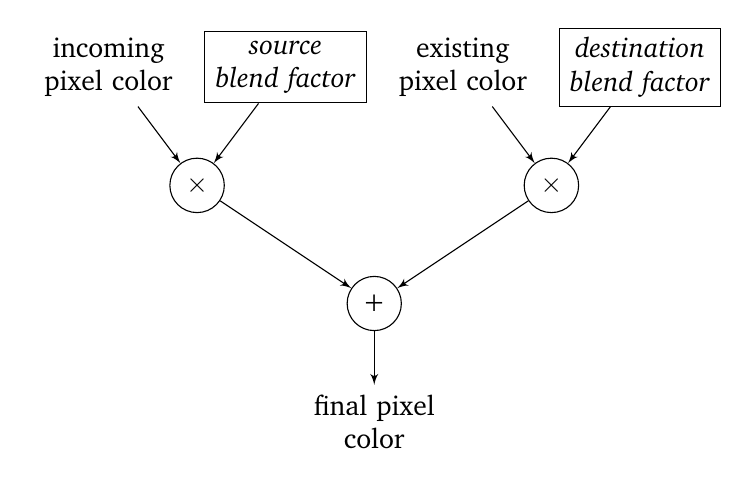
\begin{tikzpicture} [scale=0.75]
  \tikzstyle{txt}=[text width=0.15\textwidth,align=center]
  \node [txt]               at (-4.5,4) (pix) {incoming pixel color};
  \node [shape=rectangle,draw,txt] at (-1.5,4) (sbf) {\textit{source blend factor}};
  \node [txt]               at (1.5,4) (exi) {existing pixel color};
  \node [shape=rectangle,draw,txt] at (4.5,4) (dbf) {\textit{destination blend factor}};
  \node [shape=circle,draw] at (-3.0,2) (src) {$\times$};
  \node [shape=circle,draw] at (3.0,2) (dst) {$\times$};
  \node [shape=circle,draw] at (0,0) (sum) {+};
  \node [txt]               at (0,-2) (fb) {final pixel color};

  \draw [-latex'] (pix) -- (src);
  \draw [-latex'] (sbf) -- (src);
  \draw [-latex'] (exi) -- (dst);
  \draw [-latex'] (dbf) -- (dst);

  \draw [-latex'] (src) -- (sum);
  \draw [-latex'] (dst) -- (sum);
  \draw [-latex'] (sum) -- (fb);
  % \draw [-latex'] (fb) [out=0,in=120] to (dst);
\end{tikzpicture}
\end{center}

默认的模式为 \mach{BlendFunc(SRC\_ALPHA, ONE\_MINUS\_SRC\_ALPHA)} ,这种模式下,输入图像的色彩根据当前alpha通道的大小和当前屏幕内容等比例混合。

另一个常用的模式为 \mach{BlendFunc(SRC\_ALPHA, ONE)}。
\mach{ONE} 作为目标混合因子表示将引入图像的色彩直接叠加到屏幕已有的内容上,这一模式十分适用于光晕和层叠效果。
如上面的代码所示,这一模式下绘制的每个圆盘都与屏幕现有的图像进行混合,因此重合部分的亮度也是累加的。

另外还有 \mach{BlendFunc(SRC\_ALPHA, ZERO)} 这一替换模式;它将禁用透明度设定。
目标混合因子 \mach{ZERO} 表示当前屏幕画面在图像混合过程中将会被直接舍弃。

\png{0069}

\newpage
\section{字体}
\png{fonts0}

\gdtwo 的GPU内置 $16$ 种字体,字号范围为 $16\sim31$ 。
其中字号 $26\sim31$ 是含抗锯齿的高质量字体。
另外,用户可以使用资源转换器( \xref{assets} )加载TrueType格式( \mach{.ttf} )的字体。
加载后,用户可以在任意绘制指令中使用这个新字体。

\eg{fonts-night}

\begin{center}
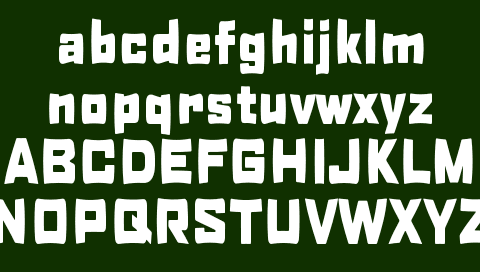
\includegraphics[width=0.7\textwidth]{assets/fonts1.png}
\end{center}

\newpage
\section{子坐标系}

自始至此,所有关于绘制点的指令都是通过调用 \dcmd{Vertex2ii} 实现的,但是 \dcmd{Vertex2ii} 只能绘制 $0\sim511$ 范围的整数坐标点 $(x,y)$。
那么如何绘制一个坐标为负值的图形或是非整数坐标点呢?
这些情况下可以调用 \dcmd{Vertex2f} ,它对于 $x$ 和 $y$ 的坐标参数有着更精细的单位和更大的取值范围。
\dcmd{Vertex2f} 坐标的单位是 $1/16$ 像素。因此,如下所示调用 \dcmd{Vertex2ii} 的代码:

\begin{framed}
\begin{verbatim}
GD.Vertex2ii(1, 100);
\end{verbatim}
\end{framed}

\noindent
当调用 \dcmd{Vertex2f} 实现时将变为:

\begin{framed}
\begin{verbatim}
GD.Vertex2f(16, 1600);
\end{verbatim}
\end{framed}

\noindent
但通常为了使代码更加简单明了,这一代码会以如下所示乘以 $16$ 的方式进行编写:
\begin{framed}
\begin{verbatim}
GD.Vertex2f(16 * 1, 16 * 100);
\end{verbatim}
\end{framed}

通过 \dcmd{Vertex2f} 绘制点( \mach{POINTS} )、线( \mach{LINES} )和矩形( \mach{RECTS} )可以更加精细。
下图中的 $16$ 个圆点是由 $y$ 坐标值依次增加 $1/16$ 像素所绘制的。
如图所示,当圆点以每次向下运动 $1/16$ 像素时,系统会对像素的阴影部分进行十分微小的调节。
这种出色的精细度将大大削减``像素颗粒''效应。

\vspace{10pt}
\noindent
\begin{tikzpicture}[scale=0.08928571428571428]
\node[anchor=south west,inner sep=0] (image) at (0,0) {
\includegraphics[width=1.0\textwidth]{assets/subpixel.png}};
\foreach \x in {0,0.1,...,11.3}
  \draw [white] (\x\textwidth,0) -- (\x\textwidth,9.6);
\foreach \y in {0,0.1,...,0.9}
  \draw [white] (0,\y\textwidth) -- (11.2\textwidth,\y\textwidth);
\end{tikzpicture}

\newpage
\section{Furmans角度}
\label{furmans}
\index{Furmans}
\index{angles!in Furmans}
\cmdidx{rsin}
\cmdidx{rcos}
\cmdidx{atan2}
\cmdidx{polar}

GD程序库在以下指令中会涉及到角度的应用:

\begin{itemize}
\item \cmd{rotate} 指令旋转图像时需要用到角度参数;
\item \cmd{dial} 指令以某一特定的角度绘制表盘控件;
\item 调用 \cmd{track} 跟踪控件时输出的转动控件的旋转角度; 
\item 数学函数\nameref{rsin} 、 \nameref{rcos} 、 \nameref{polar} 和 \nameref{atan2} 都需要使用角度参数。
\end{itemize}

上列所有情况,角度的单位都特定为Furmans角度,而不是角度和弧度。
Furman是一种角度度量单位,定义一个圆周是 $65536$ 个Furmans度。其转化关系如下列公式所示:

\[
1 \text{ Furman}
\; = \;
\frac{1}{65536} \text{ circle} 
\; = \;
\frac{360}{65536} \text{ degrees}
\; = \;
\frac{2\pi}{65536} \text{radians}
\]

角度的方向是顺时针方向,$0$ 刻度值在正下方:

\begin{center}
\begin{tikzpicture}[scale=0.75]
    \newcommand{\rb}{3.3}
    \draw (0, 0) circle (\rb);
    \draw (90:\rb) -- (90:4.0) (90:4.4) node {\mach{0x8000}};
    \draw (45:\rb) -- (45:4.0) (45:4.4) node {\mach{0xa000}};
    \draw (0:\rb) -- (0:4.0) (0:5.0) node {\mach{0xc000}};
    \draw (315:\rb) -- (315:4.0) (315:4.4) node {\mach{0xe000}};
    \draw (270:\rb) -- (270:4.0) (270:4.4) node {\mach{0}};
    \draw (225:\rb) -- (225:4.0) (225:4.4) node {\mach{0x2000}};
    \draw (180:\rb) -- (180:4.0) (180:5.0) node {\mach{0x4000}};
    \draw (135:\rb) -- (135:4.0) (135:4.4) node {\mach{0x6000}};

    % \draw (45:3.9) -- (45:4.8)     [<-, thick] node [right] {\reg{CMD\_READ}};
    % \draw (-200:3.9) -- (-200:4.8) [<-, thick] node [left] {\reg{CMD\_WRITE}};

\end{tikzpicture}
\end{center}
为了方便,GD程序库定义了一个宏函数 \mach{DEGREES()} ,它可以将角度转换成相应的Furmans角度:
\begin{verbatim}
#define DEGREES(n) ((65536UL * (n)) / 360)
\end{verbatim}

\newpage
使用Furmans角度作为单位的优点在于它可以使包含角度的数学运算更加易于计算。
例如,当增大某个旋转物体的角度时,只需要用普通的 $16$ 位运算就可表示从 $65535$ 到 $0$ 度的Furman角度运算。

\begin{center}
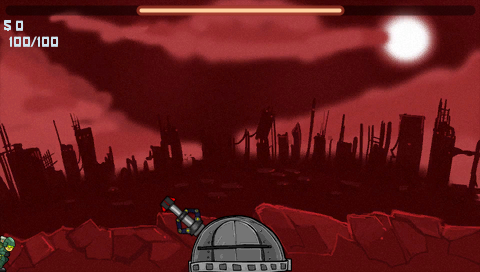
\includegraphics[width=0.7\textwidth]{assets/angle.png}
\end{center}

\index{tracking controls}
在游戏NightStrike中,
\index{NightStrike}
玩家通过触按屏幕控制炮塔的角度。
游戏启动时,游戏程序命令GPU跟踪任意触摸标签为 \mach{0x01} 的触击:
\eg{nightstrike-cmd_track}
\noindent
\cmd{track} 指令执行后, \mach{GD.inputs.track\_val}将记录下从屏幕坐标 $(240, 271)$ 到触摸点坐标这一向量的Furmans角度,之后程序再将这一数据赋值给炮塔的角度变量。
\eg{nightstrike-track}
当绘制炮塔时, \cmd{rotate} 指令将使用这一角度变量旋转炮塔的图像,
\cmdidx{cmd\_rotate}
下图为炮塔在 $0$ Furmans角度时的原图像: 
\begin{center}

\includegraphics[width=0.10\textwidth]{assets/turret.png}
\end{center}

\newpage
\section{环境堆栈}
\index{context}
\png{context}

\eg{nightstrike-context}

\textit{NightStrike} 的标题界面使用函数 \mach{blocktext}
\index{NightStrike}
来绘制带有黑色轮廓的字符串 \mach{s} 。
实现这一效果时,要使用 \dcmd{ColorRGB} 将颜色变为黑色,然后分别以左上、左下、右上、右下四个方向微小的位置偏差将文本绘制四遍。而后需要再次以文本原有的颜色绘制文本,但先前的操作已经将文本的颜色设置为黑色,导致文本原有的颜色丢失。

为了解决这个情况,在绘制前调用 \dcmd{SaveContext} 将所有的图形系统的状态 —— 包括颜色信息 —— 存储在一个私立的存储区。
之后再执行 \dcmd{RestoreContext} 便可恢复先前存储的所有属性,
这样文本的颜色也会恢复为先前调用 \dcmd{SaveContext} 时的颜色。

通过配合使用 \dcmd{SaveContext} 和 \dcmd{RestoreContext},图形系统的状态可以被保存,修改,之后再进行可以恢复。
只要未被调用,函数所存储的属性信息不会被修改。
Gameduino的GPU有足够的内存空间支持存储额外三份这样的图形属性备份。

% \section{Color, tag and stencil}
% \section{Clock}
% \section{Widgets}

%%%%%%%%%%%%%%%%%%%%%%%%%%%%%%%%%%%%%%%%%%%%%%%%%%%%%%%%%%%%%%%%%%%%%%%%
\chapter{触摸屏}

\section{读取触摸屏的输入}

函数 \nameref{getinputs} 可以读取Gameduino 2的所有输入数据,其中包括触摸传感器的输入。
调用此函数后, 你可以通过 
\mach{GD.inputs.x} 和
\mach{GD.inputs.y} 得到按击位置的相应坐标。 
程序中检测触摸输入的最佳时间是在开始绘制游戏界面之前,如下所示:

\eg{simon-touch}

没有触摸信号时, \mach{GD.inputs.x} 和 \mach{GD.inputs.y} 的值为 $-32768$ 。
触摸所得的坐标值 $(x,y)$ 是在屏幕上的像素坐标,其范围分别是
 $(0 \le x \le 479)$  和  $(0 \le y \le 271)$ ,
将此类像素坐标转换为子坐标系坐标时只需将相应数值乘以 $16$ 。如下所示:
\eg{blobs-xy}

\newpage
\section{设计实例: blobs}
\index{demos!blobs}
\png{blobs}
在演示程序``blobs''中,你可以用手指或是手写笔绘制出一连串五颜六色不断扩散的圆点。
这段代码支持连续捕捉 $128$ 个点,每个点都通过不断改变半径和透明度呈现出一种有趣的淡出效果。 

程序启动时, \mach{begin()} 函数首先将所有blobs的坐标设定在屏幕范围外。

\eg{blobs-a}

当屏幕被点击时,点击位置的子坐标系坐标将被添加至 \mach{blobs} 序列中。
各个blob的透明度和半径取决与其当前的生命周期。
所谓``随机''的颜色实际上是通过取模运算得到的。 

\eg{blobs-b}

\section{触摸标签}

作为GPU的一项特色功能,触摸标签使触摸检测变得更加轻松。
在多数情况下,触摸的具体坐标并不重要 —— 你只需关注被触摸的对象是什么。
每当你在屏幕上绘制一个对象时,你可以对该对象所包含的所有像素点赋予一个字节的编码。
例如,创建一个`OK'按钮,并对其所包含的像素点赋予代码值 $44$ 。
此后,每当用户点击这个按钮,标签寄存器中的值就会变为 $44$ 。
触摸标签值均为单字节数值,范围从 $0\sim255$ 。
不过,设备将 $255$ 这一标签值视为``无触摸产生'',因此标签值的实际可用范围为 $0\sim254$ 。

\png{0005}

下面这个例子在绘制每个数字之前设定了对应标签值,这样每个数字所含的像素点都会被标记出来。 在触摸对应数字后,\mach{GD.inputs.tag} 会被设定为当前点击的数字,Arduino可以读取出来并通过串口输出到屏幕上。

\eg{examples-h}

\newpage
\section{涂鸦}
\label{sketching}
\index{sketching}
\cmdidx{cmd\_sketch}

\png{sketching}

涂鸦在这里表示采用触摸输入在屏幕上进行绘图。
\gdtwo 的GPU已内置涂鸦功能,因此你无需通过Arduino输入任何指令即可绘制像素图像。
\cmd{sketch} 指令用于启动绘图功能,而 \cmd{stop} 指令用于停止绘图。
注意,\mach{GD.finish()} 调用会将使缓冲区的指令立即强制送入GPU中。

\eg{sketch-a}

\newpage
\section{控件与跟踪控制}
\label{widgets}
\index{widgets}
\index{tracking controls}
\index{user interface}

\png{widgets3d}

\gdtwo 有丰富的控件可供使用:仪表盘、按钮、计量器、滑动条和滚动条。
为了更好地管理与这些可调控件的交互,可以使用跟踪控制这个功能拓展前面提到的标签系统。
利用标签功能,每当相应对象被点击时程序都能够立刻得知;而通过跟踪控制,程序不仅可以得知发生了触摸事件,还可以得知触摸发生的相对位置。

\index{demos!widgets}
\mach{widgets} 例程绘制出了所有的控件类型,
并且对于其中三个可调控件——表盘,滑动条和拨动开关——使用了跟踪控制功能对它们的触控进行管理。
在这列,这三个可调控件在绘制时都被赋予独立的标签值: \mach{200} 、 \mach{201} 和 \mach{202} 。

\vspace{10pt}

\begin{tikzpicture}
  \node[anchor=south west,inner sep=0,opacity=0.2] (image) at (0,0) {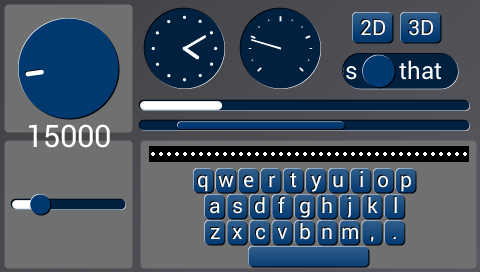
\includegraphics[width=0.9\textwidth]{assets/widgets3d.png}};
  \begin{scope}[x={(image.south east)},y={(image.north west)},xscale=0.20833333333333334,yshift=0.51\textwidth,yscale=-0.3676470588235294]

    \draw[black, thick] (0.68,0.68) circle (0.50);
    \node at (0.68,0.68) {200};

    % \draw[black, ultra thick] (0.16,1.99) rectangle (0.40);
    % \node at (0.16,1.99) {201};

    \node [draw,
      shape=rounded rectangle,
          minimum width=28mm,
          minimum height=0mm,
          ]
        at (0.68,2.04) {201};

    \node [draw,
      shape=rounded rectangle,
          minimum width=28mm,
          minimum height=8mm,
          ]
        at (4.00,0.69) {202};

  \end{scope}
\end{tikzpicture}

\newpage
之后程序命令GPU跟踪这三个可调控件区域内的触控。程序首先对表盘赋予 $200$ 的标签值,
然后调用 \cmd{track} 令GPU跟踪所有在这个标签值下的触按,并计算其对于表盘中心(屏幕坐标位置为 $(68, 68)$ )的相对位置:
\eg{widgets-dial}
\index{angles!rotary tracking}

对于线性控件如滑动条和拨动开关也有类似的控制方法:
\eg{widgets-linear}

这样之后,程序能够通过读取
\mach{GD.inputs.track\_tag} 和
\mach{GD.inputs.track\_val} 检测触摸对于任意控件的相对位置。
\mach{GD.inputs.track\_val} 中的值为无符号 $16$ 位整型数值,范围为 $0\sim65535$。
对于转动跟踪——仪表盘——该值代表对应的Furmans触按角度;而对于线性跟踪,该值代表在矩形中的触摸位置:
$0$ 代表最左端,$65535$ 代表最右端。
\eg{widgets-track}
%%%%%%%%%%%%%%%%%%%%%%%%%%%%%%%%%%%%%%%%%%%%%%%%%%%%%%%%%%%%%%%%%%%%%%%%
\chapter{声音}

\gdtwo 有两种声音系统。
第一种声音系统——音频合成器——能够生成一系列固定的声音和乐器音符。
该系统对于在程序中添加音频十分实用和便捷,但由于声音素材是固定的,因此所添加的音频灵活可变性相对较差。
第二种声音系统是采样回放,该系统能够播放存放在内存中的多种格式的音频素材。
这种系统相对来说灵活性大大增加,但你需要提前准备音频素材,并在RAM中载入所需音频。

\section{敲击音效}

音频合成器提供若干短促的``打击''音效,主要是为用户交互界面提供音效素材。
通过调用 \mach{GD.play()} 函数并提供音效素材的ID,可以触发对应的音效。
所有可用的音效列表如下所示:

\vspace{10pt}
\begin{tabular}{l}
\mach{CLICK} \\
\mach{SWITCH} \\
\mach{COWBELL} \\
\mach{NOTCH} \\
\mach{HIHAT} \\
\mach{KICKDRUM} \\
\mach{POP} \\
\mach{CLACK} \\
\mach{CHACK} \\
\end{tabular}
\vspace{10pt}

\section{乐器音符}

音频合成器也能够生成乐器音符。
同样是通过调用 \mach{GD.play()} 来触发这些音符,只是在这个情况下,第一个参数设置为了乐器的名称:

\index{instruments}
\label{instruments}

\vspace{10pt}
\begin{tabular}{l}
\mach{HARP} \\
\mach{XYLOPHONE} \\
\mach{TUBA} \\
\mach{GLOCKENSPIEL} \\
\mach{ORGAN} \\
\mach{TRUMPET} \\
\mach{PIANO} \\
\mach{CHIMES} \\
\mach{MUSICBOX} \\
\mach{BELL}
\end{tabular}
\vspace{10pt}

\noindent
这种情况下, \mach{GD.play()} 还可以接受一个额外的参数,用于设置MIDI音符号,其范围为 $21\sim108$。
当该参数空缺时,程序默认播放C4的音效,即MIDI音符 $60$ 。

音频合成器还可以播放一些其他的音效。
乐音
\mach{SQUAREWAVE},
\mach{SINEWAVE},
\mach{SAWTOOTH} 和
\mach{TRIANGLE} 
能够合成简单的连续波形,这可以用于产生老式游戏的音效感。
乐音
\mach{BEEPING},
\mach{ALARM},
\mach{WARBLE} 和
\mach{CAROUSEL}
能够合成各式各样的警报音效。
另外,ASCII代码 `0'-`9', `*' 和 `\#' 能够生成对应的DTMF音效(电话机的播号音效)。

通过读取设备的 \mach{PLAY} 寄存器可以检测声音是否播放结束。
当此寄存器内数值为 $0$ 时,代表声音已经播放结束:
\eg{examples-waitnote}

\tablefirsthead{%
MIDI 音符 & ANSI 音符 & 频率. (Hz) \\
\hline
}
\tablehead{%
MIDI 音符 & ANSI 音符 & 频率. (Hz) \\
\hline
}
\footnotesize
\twocolumn
\begin{spacing}{0.99}
\begin{supertabular}{ccc}
\index{MIDI notes|boldindex}
\label{MIDI}
21  & A0  &  27.5 \\
22  & A$^\#$0 &  29.1 \\
23  & B0  &  30.9 \\
24  & C1  &  32.7 \\
25  & C\#1 &  34.6 \\
26  & D1  &  36.7 \\
27  & D\#1 &  38.9 \\
28  & E1  &  41.2 \\
29  & F1  &  43.7 \\
30  & F\#1 &  46.2 \\
31  & G1  &  49.0 \\
32  & G\#1 &  51.9  \\
33  & A1  &  55.0  \\
34  & A\#1 &  58.3  \\
35  & B1  &  61.7  \\
36  & C2  &  65.4  \\
37  & C\#2 &  69.3  \\
38  & D2  &  73.4  \\
39  & D\#2 &  77.8  \\
40  & E2  &  82.4  \\
41  & F2  &  87.3  \\
42  & F\#2 &  92.5  \\
43  & G2  &  98.0  \\
44  & G\#2 & 103.8  \\
45  & A2  & 110.0  \\
46  & A\#2 & 116.5  \\
47  & B2  & 123.5  \\
48  & C3  & 130.8  \\
49  & C\#3 & 138.6  \\
50  & D3  & 146.8  \\
51  & D\#3 & 155.6  \\
52  & E3  & 164.8  \\
53  & F3  & 174.6  \\
54  & F\#3 & 185.0  \\
55  & G3  & 196.0  \\
56  & G\#3 & 207.7  \\
57  & A3  & 220.0  \\
58  & A\#3 & 233.1  \\
59  & B3  & 246.9  \\
60  & C4  & 261.6  \\
61  & C\#4 & 277.2  \\
62  & D4  & 293.7  \\
63  & D\#4 & 311.1  \\
64  & E4  & 329.6  \\
65  & F4  & 349.2  \\
66  & F\#4 & 370.0  \\
67  & G4  & 392.0  \\
68  & G\#4 & 415.3  \\
69  & A4  & 440.0  \\
70  & A\#4 & 466.2  \\
71  & B4  & 493.9  \\
72  & C5  & 523.3  \\
73  & C\#5 & 554.4  \\
74  & D5  & 587.3  \\
75  & D\#5 & 622.3  \\
76  & E5  & 659.3  \\
77  & F5  & 698.5  \\
78  & F\#5 & 740.0  \\
79  & G5  & 784.0  \\
80  & G\#5 & 830.6  \\
81  & A5  & 880.0  \\
82  & A\#5 & 932.3  \\
83  & B5  & 987.8  \\
84  & C6  & 1046.5 \\
85  & C\#6 & 1108.7 \\
86  & D6  & 1174.7 \\
87  & D\#6 & 1244.5 \\
88  & E6  & 1318.5 \\
89  & F6  & 1396.9 \\
90  & F\#6 & 1480.0 \\
91  & G6  & 1568.0 \\
92  & G\#6 & 1661.2 \\
93  & A6  & 1760.0 \\
94  & A\#6 & 1864.7 \\
95  & B6  & 1975.5 \\
96  & C7  & 2093.0 \\
97  & C\#7 & 2217.5 \\
98  & D7  & 2349.3 \\
99  & D\#7 & 2489.0 \\
100 & E7  & 2637.0 \\
101 & F7  & 2793.8 \\
102 & F\#7 & 2960.0 \\
103 & G7  & 3136.0 \\
104 & G\#7 & 3322.4 \\
105 & A7  & 3520.0 \\
106 & A\#7 & 3729.3 \\
107 & B7  & 3951.1 \\
108 & C8  & 4186.0 \\
\end{supertabular}
\end{spacing}
\onecolumn
\normalsize

\section{采样回放}
\index{samples}

\gdtwo 的声音系统还可以进行采样回放。
采样回放系统是独立的——你可以在播放固定音符的同时播放音频素材,
而设备将会通过分配好的音量将它们混合在一起进行播放。

调用 \mach{GD.sample} 可以播放内存中的采样音频。 该函数设置的参数有:音频的基准地址,音频文件大小,频率以及格式。
举例来说,若要播放一段位于地址 $0$ ,音频文件大小为 $22050$ 字节,频率为 $44100$ Hz的ULAW格式的音频,程序如下:

\begin{framed}
\begin{verbatim}
GD.sample(0, 22050, 44100, ULAW_SAMPLES);
\end{verbatim}
\end{framed}

采样回放系统支持3种音频格式:

\vspace{10pt}
\begin{tabular}{ccl}
格式 & 音频位数 & 音频编码 \\
\hline \\
\mach{LINEAR\_SAMPLES} & 8 & 有符号 $8$ 位线性, $-128$ - $127$ \\
\mach{ULAW\_SAMPLES} & 8 & 标准 $8$ 位$\mu$-law编码 \\
\mach{ADPCM\_SAMPLES} & 4 & 标准IMA ADPCM编码 \\
\end{tabular}
\vspace{10pt}

\gdtwo 的资源转换器( \xref{assets} )可以将单声道的 \mach{.wav} 文件转换成上述任意格式。
硬件设备最高可以支持 $48$ kHz的采样率,在此频率下,ADPCM格式音频素材的声音质量和AM收音机等同。
当然,在此频率下的音频所占内存的大小也很高,大约是 $24$ kBytes/s。
为了节省内存,最好采用较低采样率的ADPCM音频。 \mach{noisy} 例程播放了数字 $0$ 至 $9$ 的音频采样,采样率为 $8$ kHz,编码格式为ADPCM。
这些采样的声音简单明了,总共只占了 $26$ kBytes的显存。

值得注意的是,\mach{GD.sample()} 对于参数有一个强制限制,那就是基准地址的长度必须是 $8$ 的倍数。
不过资源转换器会自动对采样音频进行校准,所以用户对此不需再做什么特殊操作。

\newpage
\eg{noisy-A}

\newpage
\section{连续播放}

\png{song}

对于较长的音频,将整个音频采样存入内存通常不现实。
取而代之的是,可以使用采样回放系统通过循环来播放一段音频。在这个情况下,Arduino不断读取SD卡,并并更新需要播放的音频。
GD2程序库中的 \mach{Streamer} 类可以十分轻松的管理这些细节。
首先,调用它的 \mach{begin()} 方法,并以microSD卡上音频文件的名字作为参数。
\mach{Streamer} 默认情况下采用采样率为 $44.1$ kHz的IMA ADPCM的采样编码。
音频流使用 $4$ K的缓存,这些缓存被安排于显存中的顶端。

调用 \mach{Streamer} 的 \mach{feed()} 方法从文件中读取音频采样,并更新至缓存中。
应用程序应时常调用 \mach{feed()} 以防止缓存中的音频采样耗尽。
在下例中,程序每一帧都会调用一次 \mach{stream.feed()} 。

\mach{Streamer} 还可以获知音频播放进程已经进行到什么位置。
\mach{progress()} 将会返回一对16位的数字,
\mach{val} 和 \mach{range} ,而当前已经播放的进程比例可以通过 $(\mach{val} / \mach{range})$ 计算而来。
在下面的例程中,程序直接将 \mach{val} 和 \mach{range} 作为滑动条( \cmd{slider} )的控件参数。

如果有已安装的 \mach{sox} 音频编辑工具, 可以将 \mach{.wav} 格式的音频转换为 ADPCM IMA格式, 相应命令行如下所示:

\begin{framed}
\begin{verbatim}
$ sox mesmeriz.wav -c 1 mesmeriz.ima
$ play -r 44100 mesmeriz.ima
\end{verbatim}
\end{framed}

最后,\mach{play} 将播放转换后的音频文件。
由于 \mach{.ima} 格式没有文件头区域,而对于 \mach{play} 来说需要得知采样率才可以进行播放,所以在此手动设定为 $44100$ Hz。

\eg{song-A}

%%%%%%%%%%%%%%%%%%%%%%%%%%%%%%%%%%%%%%%%%%%%%%%%%%%%%%%%%%%%%%%%%%%%%%%%
\chapter{加速度传感器}

\begin{center}
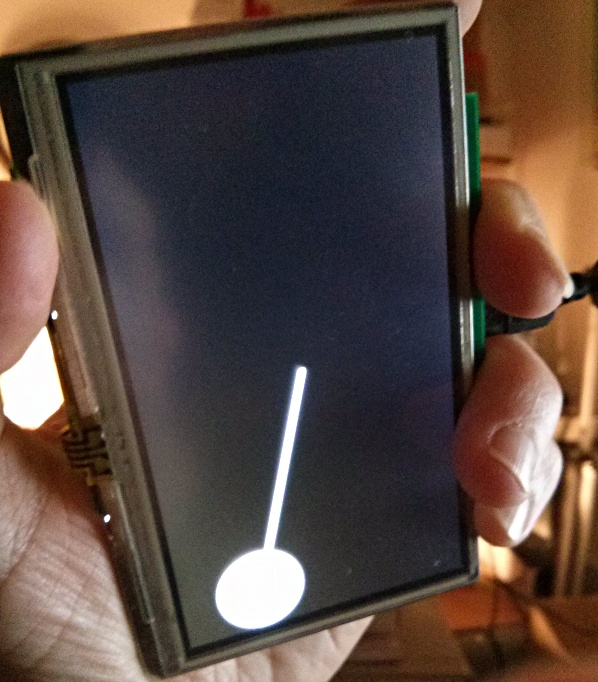
\includegraphics[width=0.4\textwidth]{assets/accel.jpg}
\end{center}

\gdtwo 还包含一个三轴加速度传感器,该传感器的输出直接连接到Arduino的A0, A1和A2模拟输入引脚上。用户可以通过\dcmd{getaccel} 
函数来获取当前的加速度大小:

\begin{framed}
\begin{verbatim}
int x, y, z;
GD.get_accel(x, y, z);
\end{verbatim}
\end{framed}

\noindent
\mach{get\_accel()} 函数对输出结果进行了矫正,将单位重力在
\mach{x},
\mach{y} 或
\mach{z} 轴上的分量大小调整为 $256$ 。
如果将 \gdtwo 完全倾向左侧,就会得到以下数值:
\mach{x} = $-256$,
\mach{y} = $0$,
\mach{z} =$0$。
因为该加速度传感器是模拟量输入,所以这些值会存在一些误差。
在示例程序 \mach{tilt} 中,你将看到在加速度传感器的输出中就会存在一些微小的 ``噪声''。

\eg{tilt-A}

%%%%%%%%%%%%%%%%%%%%%%%%%%%%%%%%%%%%%%%%%%%%%%%%%%%%%%%%%%%%%%%%%%%%%%%%
\chapter{MicroSD卡}

\gdtwo 包含一个标准microSD卡接口。
它与 \gdtwo 的GPU芯片共用一组SPI接口,并通过Arduino的数字引脚9进行使能。
现在有很多程序库可以用于驱动microSD卡,而GD程序库包含了一个相对轻量级的程序库。
该程序库可以用于驱动FAT格式的microSD卡,并且与GD图形系统无缝集成。

MicroSD的文件经常被直接输入到GPU的命令流中。
\mach{GD.load()} 命令就是如此的,它的工作流程是:该函数从SD中读取一个文件,并把它的内容传送到
\gdtwo 的GPU中。
举一个例子,用户可以通过以下指令来载入一张JPEG格式的图片:

\begin{framed}
\begin{verbatim}
GD.cmd_loadimage(0);
GD.load("kitten.jpg");
\end{verbatim}
\end{framed}

\noindent
函数 \cmd{loadimage} 告知GPU准备接收一个JPEG图片,之后 \nameref{load} 函数将图片数据全部读取到GPU中。

下面是另外一个例子,演示了如何从SD卡的`` \mach{mem.raw} ''文件中读取 $16$KB的原始数据:

\begin{framed}
\begin{verbatim}
GD.cmd_memwrite(0, 16384);
GD.load("mem.raw");
\end{verbatim}
\end{framed}

\noindent
同样的,此处 \cmd{memwrite} 告知GPU准备接收数据,之后由 \nameref{load} 函数将数据装载至GPU中。

由对象转化器( \xref{assets} )生成的 \mach{.gd2} 格式文件为纯命令流,也可以通过 \nameref{load}
函数载入:

\begin{framed}
\begin{verbatim}
GD.load("frogger.gd2");
\end{verbatim}
\end{framed}

\noindent
通过该命令,所有 \mach{frogger} 游戏需要的图形元素就被载入到了内存中,并同时设置好了相应的位图句柄。
在对象转换器生成的头文件 \mach{frogger\_assets.h} 中,包含了以下的宏定义:

\begin{framed}
\begin{verbatim}
#define LOAD_ASSETS()   GD.load("frogger.gd2")
\end{verbatim}
\end{framed}

\noindent
所以在 \mach{frogger} 的程序中,只需简单地在 \mach{setup()} 
函数中调用 \mach{LOAD\_ASSETS()} 就可以载入所有的图形资源了。

% \section{Reading files}
% \section{Reading directories}


\part{编程参考}

%%%%%%%%%%%%%%%%%%%%%%%%%%%%%%%%%%%%%%%%%%%%%%%%%%%%%%%%%%%%%%%%%%%%%%%%
\chapter{绘图指令}

\newcommand{\drawcmd}[2]{
\newpage
\section{\texttt{#1}}
\label{#1}
\index{#1@\mach{#1()}|boldindex}

#2

}

\newcommand{\lightcmd}[3]{
\section{\texttt{#1}}
\label{#2}
\index{#1@\mach{#1()}|boldindex}


}

\drawcmd{AlphaFunc}{Sets the alpha-test function}

\begin{framed}
\begin{verbatim}
void AlphaFunc(byte func,
               byte ref);
\end{verbatim}
\end{framed}

\begin{tabular}{lp{0.8 \textwidth}}

\\ \mach{func} & comparison function, one of
        \mach{NEVER}, \mach{LESS}, \mach{LEQUAL}, \mach{GREATER}, \mach{GEQUAL}, \mach{EQUAL}, \mach{NOTEQUAL}, or \mach{ALWAYS} \\

\\ \mach{ref} & reference value for comparison function \\

\end{tabular}

\vspace{10pt}
The alpha test function tests each pixel's
alpha value, and only draws the pixel
if the test passes.
For example
\begin{verbatim}
  GD.AlphaText(GEQUAL, 160);
\end{verbatim}
means that only pixels with $(A \ge 160)$ are drawn.  
The default state is \mach{ALWAYS}, which means that pixels are always drawn.
\minipng{0032}
\eg{examples-alphafunc}

\drawcmd{Begin}{Selects the graphics primitive for drawing}

\begin{framed}
\begin{verbatim}
void Begin(byte prim);
\end{verbatim}
\end{framed}

\begin{tabular}{lp{0.8 \textwidth}}

\\ \mach{prim} & one of
\mach{BITMAPS},
\mach{POINTS},
\mach{LINES},
\mach{LINE\_STRIP},
\mach{EDGE\_STRIP\_R},
\mach{EDGE\_STRIP\_L},
\mach{EDGE\_STRIP\_A},
\mach{EDGE\_STRIP\_B} or
\mach{RECTS} \\
\end{tabular}

\vspace{10pt}
The \mach{Begin} command sets the current graphics draw primitve.
It does not draw anything - that is done by a later \nameref{Vertex2f} or \nameref{Vertex2ii} command.
The drawing primitive can be:

\vspace{10pt}

\begin{tabular}{lp{0.8 \textwidth}}
\mach{BITMAPS     } & each vertex draws a bitmap \\
\mach{POINTS      } & each vertex draws an anti-aliased point  \\
\mach{LINES       } & each pair of vertices draws an anti-aliased line \\
\mach{RECTS       } & each pair of vertices draws an anti-aliased rectangle \\
\mach{LINE\_STRIP  } & the vertices define a connected line segment \\
\mach{EDGE\_STRIP\_A} & like \mach{LINE\_STRIP}, but draws pixels above the line \\
\mach{EDGE\_STRIP\_B} & like \mach{LINE\_STRIP}, but draws pixels below the line \\
\mach{EDGE\_STRIP\_L} & like \mach{LINE\_STRIP}, but draws pixels left of the line \\
\mach{EDGE\_STRIP\_R} & like \mach{LINE\_STRIP}, but draws pixels right of the line
\end{tabular}

\png{0047}

\drawcmd{BitmapHandle}{Sets the bitmap handle}

\begin{framed}
\begin{verbatim}
void BitmapHandle(byte handle);
\end{verbatim}
\end{framed}

\begin{tabular}{lp{0.8 \textwidth}}

\\ \mach{handle} & integer handle number, 0-15 \\

\end{tabular}

\vspace{10pt}
The \mach{BitmapHandle} command sets the current bitmap handle, used by
\nameref{Vertex2f},
\nameref{BitmapSource},
\nameref{BitmapLayout} and
\nameref{BitmapSize}.

The bitmap handle is part of the graphics context; its default value is 0.



\drawcmd{BitmapLayout}{Sets the bitmap layout}

\begin{framed}
\begin{verbatim}
void BitmapLayout(byte format,
                  uint16_t linestride,
                  uint16_t height);
\end{verbatim}
\end{framed}

\begin{tabular}{lp{0.8 \textwidth}}

\\ \mach{format} & pixel format of the bitmap, one of:
\mach{ARGB1555},
\mach{L1},
\mach{L4},
\mach{L8},
\mach{RGB332},
\mach{ARGB2},
\mach{ARGB4},
\mach{RGB565},
\mach{PALETTED},
\mach{TEXT8X8},
\mach{TEXTVGA},
\mach{BARGRAPH}.
\\

\\ \mach{linestride} & the size in bytes of one line of the bitmap in memory \\

\\ \mach{height} & height of the bitmap in pixels \\

\end{tabular}

\vspace{10pt}
The \mach{BitmapLayout} command sets the current bitmap's layout in memory.
The \mach{format} controls how memory data is converted into pixels. 
Each pixel in memory is 1,4,8 or 16 bits. The color is extracted from these bits as follows,
where ``v'' is the pixel data.

\vspace{10pt}
\begin{tabular}{cccccc}
format           & bits per & alpha        & red   & green & blue \\
                 &  pixel   &              &       &       &      \\
\hline
\mach{L1}        &    1     & v$_0$        &  1.0  &  1.0  &  1.0 \\
\mach{L4}        &    4     & v$_{3..0}$   &  1.0  &  1.0  &  1.0 \\
\mach{L8}        &    8     & v$_{7..0}$   &  1.0  &  1.0  &  1.0 \\
\hline
\mach{RGB332}    &    8     & 1.0          &  v$_{7..5}$   &  v$_{4..2}$  &  v$_{1..0}$ \\
\mach{RGB565}    &    16    & 1.0          &  v$_{15..1}$  &  v$_{10..5}$ &  v$_{4..0}$ \\
\hline
\mach{ARGB2}     &    8     & v$_{7..6}$   &  v$_{5..4}$   &  v$_{3..2}$  &  v$_{1..0}$ \\
\mach{ARGB4}     &    16    & v$_{15..12}$ &  v$_{11..8}$  &  v$_{7..4}$  &  v$_{3..0}$ \\
\end{tabular}
\vspace{10pt}

1 and 4 bit pixels are packed in bytes from left to right, so
leftmost pixels in the bitmap occupy the most significant bits in a byte.
16 bit pixels are little-endian in graphics memory, and must be aligned on even memory boundaries.

\mach{PALETTED} format uses 8 bits per pixel, each pixel is an index
into the 256 entry 32-bit color table loaded at \mach{RAM\_PALETTE}.
% \mach{TEXT8X8} interpret each byte in the bitmap as an index into a character array, with a character size of 8x8 pixels.
% \mach{TEXTVGA} interprets memory in the same format as an IBM PC VGA graphic controller, 8 bits of character attribute and an 8-bit character code. The character size is 8x16.


\drawcmd{BitmapSize}{Sets the bitmap size and appearance}

\begin{framed}
\begin{verbatim}
void BitmapSize(byte filter,
                byte wrapx,
                byte wrapy,
                uint16_t width,
                uint16_t height);
\end{verbatim}
\end{framed}

\begin{tabular}{lp{0.8 \textwidth}}

\\ \mach{filter} & bitmap pixel filtering, \mach{NEAREST} or \mach{BILINEAR} \\

\\ \mach{wrapx} & $x$ wrapping mode, \mach{BORDER} or \mach{REPEAT} \\

\\ \mach{wrapy} & $y$ wrapping mode, \mach{BORDER} or \mach{REPEAT} \\

\\ \mach{width} & on-screen drawn width, in pixels \\

\\ \mach{height} & on-screen drawn height, in pixels \\

\end{tabular}

\vspace{10pt}
The \mach{BitmapSize} command controls how the current bitmap appears on screen.



\drawcmd{BitmapSource}{Sets the bitmap source address}

\begin{framed}
\begin{verbatim}
void BitmapSource(uint32_t addr);
\end{verbatim}
\end{framed}

\begin{tabular}{lp{0.8 \textwidth}}

\\ \mach{addr} & base address for bitmap \mach{0x00000} - \mach{0x3ffff} \\

\end{tabular}

\vspace{10pt}
The \mach{BitmapSource} command sets the base address for the bitmap.
For 16-bit bitmaps, this address must be even.



\drawcmd{BlendFunc}{Sets the color blend function}

\begin{framed}
\begin{verbatim}
void BlendFunc(byte src,
               byte dst);
\end{verbatim}
\end{framed}

\begin{tabular}{lp{0.8 \textwidth}}

\\ \mach{src} & source blend factor, one of
\mach{ZERO},
\mach{ONE},
\mach{SRC\_ALPHA},
\mach{DST\_ALPHA},
\mach{ONE\_MINUS\_SRC\_ALPHA},
\mach{ONE\_MINUS\_DST\_ALPHA}.  \\

\\ \mach{dst} & destination blend factor, one of
\mach{ZERO},
\mach{ONE},
\mach{SRC\_ALPHA},
\mach{DST\_ALPHA},
\mach{ONE\_MINUS\_SRC\_ALPHA},
\mach{ONE\_MINUS\_DST\_ALPHA}.  \\

\end{tabular}

\vspace{10pt}
The \mach{BlendFunc} command sets the blend function used to combine pixels
with the contents of the frame buffer.
Each incoming pixel's color is multiplied by the source blend factor, and each frame buffer pixel
is multiplied by the destination blend factor.
These two results are added to give the final pixel color.

\minipng{0031}
\eg{examples-blendfunc}


% \drawcmd{Call}{Something}
% 
% \begin{framed}
% \begin{verbatim}
% void Call(uint16_t dest);
% \end{verbatim}
% \end{framed}
% 
% \begin{tabular}{lp{0.8 \textwidth}}
% 
% \\ \mach{dest} & something \\
% 
% \end{tabular}
% 
% \vspace{10pt}
% The \mach{Call} command

\drawcmd{Cell}{Sets the bitmap cell}

\begin{framed}
\begin{verbatim}
void Cell(byte cell);
\end{verbatim}
\end{framed}

\begin{tabular}{lp{0.8 \textwidth}}

\\ \mach{cell} & cell number 0-127 \\

\end{tabular}

\vspace{10pt}
The \mach{Cell} command sets the current bitmap cell used by the \nameref{Vertex2f} command.

\png{0034}
\eg{examples-cell}


\drawcmd{ClearColorA}{Sets the alpha component of the clear color}

\begin{framed}
\begin{verbatim}
void ClearColorA(byte alpha);
\end{verbatim}
\end{framed}

\begin{tabular}{lp{0.8 \textwidth}}

\\ \mach{alpha} & Clear color alpha component, 0-255 \\

\end{tabular}

\vspace{10pt}
The \mach{ClearColorA} command sets the clear color A channel value.
A subsequent \nameref{Clear} writes this value to the frame buffer alpha channel.



\drawcmd{Clear}{Clears the screen}

\begin{framed}
\begin{verbatim}
void Clear(byte c = 1,
           byte s = 1,
           byte t = 1);
\end{verbatim}
\end{framed}

\begin{tabular}{lp{0.8 \textwidth}}

\\ \mach{c} & if set, clear the color buffer \\

\\ \mach{s} & if set, clear the stencil buffer \\

\\ \mach{t} & if set, clear the tag buffer \\

\end{tabular}

\vspace{10pt}
The \mach{Clear} command clears the requested frame buffers.

\png{0035}
\eg{examples-clear}


\drawcmd{ClearColorRGB}{Sets the R,G,B components of the clear color}

\begin{framed}
\begin{verbatim}
void ClearColorRGB(byte red,
                   byte green,
                   byte blue);
void ClearColorRGB(uint32_t rgb);
\end{verbatim}
\end{framed}

\begin{tabular}{lp{0.8 \textwidth}}

\\ \mach{red} & red component 0-255 \\

\\ \mach{green} & green component 0-255 \\

\\ \mach{blue} & blue component 0-255 \\

\\ \mach{rgb} & 24-bit color in RGB order, \mach{0x000000}-\mach{0xffffff} \\

\end{tabular}

\vspace{10pt}
The \mach{ClearColorRGB} command sets the clear color R,G and B values.
A subsequent \nameref{Clear} writes this value to the frame buffer R,G and B channels.
\minipng{0030}
\eg{examples-clearcolorrgb}



\drawcmd{ClearStencil}{Sets the stencil clear value}

\begin{framed}
\begin{verbatim}
void ClearStencil(byte s);
\end{verbatim}
\end{framed}

\begin{tabular}{lp{0.8 \textwidth}}

\\ \mach{s} & stencil buffer clear value 0-255 \\

\end{tabular}

\vspace{10pt}
The \mach{ClearStencil} command sets the stencil buffer clear value.
A subsequent \nameref{Clear} writes this value to the stencil buffer.



\drawcmd{ClearTag}{Sets the tag clear value}

\begin{framed}
\begin{verbatim}
void ClearTag(byte s);
\end{verbatim}
\end{framed}

\begin{tabular}{lp{0.8 \textwidth}}

\\ \mach{s} & tag value 0-255 \\

\end{tabular}

\vspace{10pt}
The \mach{ClearTag} command sets the tag buffer clear value.
A subsequent \nameref{Clear} writes this value to the tag buffer.



\drawcmd{ColorA}{Sets the A component of the current color}

\begin{framed}
\begin{verbatim}
void ColorA(byte alpha);
\end{verbatim}
\end{framed}

\begin{tabular}{lp{0.8 \textwidth}}

\\ \mach{alpha} & alpha value 0-255 \\

\end{tabular}

\vspace{10pt}
The \mach{ColorA} command sets the alpha component of the current drawing color.
\png{0029}
\eg{examples-colora}

\drawcmd{ColorMask}{Sets the mask controlling color channel writes}

\begin{framed}
\begin{verbatim}
void ColorMask(byte r,
               byte g,
               byte b,
               byte a);
\end{verbatim}
\end{framed}

\begin{tabular}{lp{0.8 \textwidth}}

\\ \mach{r} & if set, enable writes to the red component \\

\\ \mach{g} & if set, enable writes to the green component \\

\\ \mach{b} & if set, enable writes to the blue component \\

\\ \mach{a} & if set, enable writes to the alpha component \\

\end{tabular}

\vspace{10pt}
The \mach{ColorMask} command sets the color mask, which enables color writes to the frame buffer
R,G,B and A components.

\minipng{0033}
\eg{examples-colormask}


\drawcmd{ColorRGB}{Sets the R,G,B components of the current color}

\begin{framed}
\begin{verbatim}
void ColorRGB(byte red,
              byte green,
              byte blue);

void ColorRGB(uint32_t rgb);
\end{verbatim}
\end{framed}

\begin{tabular}{lp{0.8 \textwidth}}

\\ \mach{red} & red component 0-255 \\

\\ \mach{green} & green component 0-255 \\

\\ \mach{blue} & blue component 0-255 \\

\\ \mach{rgb} & 24-bit color in RGB order, \mach{0x000000}-\mach{0xffffff} \\

\end{tabular}

\vspace{10pt}
The \mach{ColorRGB} command sets the current color.
This color is used by all drawing operations.

\minipng{0028}
\eg{examples-colorrgb}


\drawcmd{LineWidth}{Set the line width}

\begin{framed}
\begin{verbatim}
void LineWidth(uint16_t width);
\end{verbatim}
\end{framed}

\begin{tabular}{lp{0.8 \textwidth}}

\\ \mach{width} & line width in $1/16$th of a pixel \\

\end{tabular}

\vspace{10pt}
The \mach{LineWidth} command sets the line width used when drawing \mach{LINES} and \mach{LINE\_STRIP}.
The width is specified in $1/16$th of a pixel, so
\mach{LineWidth(16)} sets the width to 1 pixel.
Note that the width is the distance from the center of the line to its outside edge,
rather like the radius of a circle. So the total width of the line is double the value specified.

The maximum line width is 4095, or $255 \frac{15}{16}$ pixels.
\png{0026}
\eg{examples-linewidth}

\drawcmd{PointSize}{Set the point size}

\begin{framed}
\begin{verbatim}
void PointSize(uint16_t size);
\end{verbatim}
\end{framed}

\begin{tabular}{lp{0.8 \textwidth}}

\\ \mach{size} & point size in $1/16$th of a pixel \\

\end{tabular}

\vspace{10pt}
The \mach{PointSize} command sets the point size used when drawing \mach{POINTS}.
The size is specified in $1/16$th of a pixel, so
\mach{LineWidth(16)} sets the width to 1 pixel.
Note that the size is the distance from the center of the point to its outside edge,
that is, the radius. So the total width of the point is double the value specified.

The maximum point size is 4095, or $255 \frac{15}{16}$ pixels.
\png{0027}
\eg{examples-pointsize}


\drawcmd{RestoreContext}{Restore the drawing context to a previously saved state}

\begin{framed}
\begin{verbatim}
void RestoreContext(void);
\end{verbatim}
\end{framed}

\begin{tabular}{lp{0.8 \textwidth}}

\end{tabular}

\vspace{10pt}
The collected graphics state is called the \textit{graphics context}.
The \mach{SaveContext} command saves a copy of this state, and the \mach{RestoreContext} command restores this saved copy.

The hardware can preserve up to four graphics contexts in this way. The graphics context consists of:
\vspace{10pt}

\begin{tabular}{rl}
state & drawing commands \\
\hline
alpha-test function   &  \nameref{AlphaFunc} \\
bitmap handle         &  \nameref{BitmapHandle} \\
blend function        &  \nameref{BlendFunc} \\
bitmap cell           &  \nameref{Cell} \\
color clear value     & \nameref{ClearColorA}, \nameref{ClearColorRGB} \\
stencil clear value   & \nameref{ClearStencil} \\
tag clear value       & \nameref{ClearTag} \\
color write mask      & \nameref{ColorMask} \\
color                 & \nameref{ColorA}, \nameref{ColorRGB} \\
line width            & \nameref{LineWidth} \\
point size            & \nameref{PointSize} \\
scissor rectangle     & \nameref{ScissorSize}, \nameref{ScissorXY} \\
stencil test function & \nameref{StencilFunc} \\
stencil write mask    & \nameref{StencilMask} \\
stencil operation     & \nameref{StencilOp} \\
tag write mask        & \nameref{TagMask} \\
tag value             & \nameref{Tag}
\end{tabular}



\drawcmd{SaveContext}{Save the graphics context}

\begin{framed}
\begin{verbatim}
void SaveContext(void);
\end{verbatim}
\end{framed}

\begin{tabular}{lp{0.8 \textwidth}}

\end{tabular}

\vspace{10pt}
The collected graphics state is called the \textit{graphics context}.
The \mach{SaveContext} command saves a copy of this state, and the \mach{RestoreContext} command restores this saved copy.

\png{0036}
\eg{examples-context}

\drawcmd{ScissorSize}{Set the size of the scissor rectangle}

\begin{framed}
\begin{verbatim}
void ScissorSize(uint16_t width,
                 uint16_t height);
\end{verbatim}
\end{framed}

\begin{tabular}{lp{0.8 \textwidth}}

\\ \mach{width} & scissor rectangle width, in pixels, 0-512 \\

\\ \mach{height} & scissor rectangle height, in pixels, 0-512 \\

\end{tabular}

\vspace{10pt}
The \mach{ScissorSize} command sets the dimensions of the scissor rectangle.
The scissor rectangle limits drawing to a rectangular region on the screen.

\png{0037}
\eg{examples-scissor}


\drawcmd{ScissorXY}{Set the top-left corner of the scissor rectangle}

\begin{framed}
\begin{verbatim}
void ScissorXY(uint16_t x,
               uint16_t y);
\end{verbatim}
\end{framed}

\begin{tabular}{lp{0.8 \textwidth}}

\\ \mach{x} & $x$ coordinate of top-left corner of the scissor rectangle, 0-511 \\

\\ \mach{y} & $y$ coordinate of top-left corner of the scissor rectangle, 0-511 \\

\end{tabular}

\vspace{10pt}
The \mach{ScissorXY} command sets the top-left corner of the scissor rectangle.
The scissor rectangle limits drawing to a rectangular region on the screen.


\drawcmd{StencilFunc}{Set the stencil test function}

\begin{framed}
\begin{verbatim}
void StencilFunc(byte func,
                 byte ref,
                 byte mask);
\end{verbatim}
\end{framed}

\begin{tabular}{lp{0.8 \textwidth}}

\\ \mach{func} & set the stencil comparison operation, one of
        \mach{NEVER}, \mach{LESS}, \mach{LEQUAL}, \mach{GREATER}, \mach{GEQUAL}, \mach{EQUAL}, \mach{NOTEQUAL}, or \mach{ALWAYS} \\

\\ \mach{ref} & set the stencil reference value used for the comparison, 0-255 \\

\\ \mach{mask} & an 8-bit mask that is anded with both \mach{ref} and the pixel's stencil value before comparison, 0-255 \\

\end{tabular}

\vspace{10pt}
The \mach{StencilFunc} command controls the stencil testing operation.
During drawing, the stencil test is applied to each pixel, and if the test fails, the pixel is not drawn.
Setting \mach{func} to \mach{ALWAYS} means that pixels are always drawn.

\drawcmd{StencilMask}{Sets the mask controlling stencil writes}

\begin{framed}
\begin{verbatim}
void StencilMask(byte mask);
\end{verbatim}
\end{framed}

\begin{tabular}{lp{0.8 \textwidth}}

\\ \mach{mask} & Each set bit enables the corresponding bit write to the stencil buffer \\

\end{tabular}

\vspace{10pt}
The \mach{StencilMask} command controls writes to the stencil buffer.
Because the stencil buffer is 8 bits deep, each bit in \mach{mask} enables writes to the same bit of the stencil buffer.
So a \mach{mask} of \mach{0x00} disables stencil writes, and a \mach{mask} of \mach{0xff} enables stencil writes.


\drawcmd{StencilOp}{Set the stencil update operation}

\begin{framed}
\begin{verbatim}
void StencilOp(byte sfail,
               byte spass);
\end{verbatim}
\end{framed}

\begin{tabular}{lp{0.8 \textwidth}}

\\ \mach{sfail} & the operation to be applied to pixels that fail the stencil test.
One of \mach{ZERO}, \mach{KEEP}, \mach{REPLACE}, \mach{INCR}, \mach{DECR} or \mach{INVERT}.

\\ \mach{spass} & the operation to be applied to pixels that pass the stencil test.
One of \mach{ZERO}, \mach{KEEP}, \mach{REPLACE}, \mach{INCR}, \mach{DECR} or \mach{INVERT}.

\end{tabular}

\vspace{10pt}
The \mach{StencilOp} command controls how drawn pixels modify the stencil buffer.
If the the pixel failed the stencil test, then the operation specified by \mach{sfail} is performed.
Otherwise the operation \mach{spass} is performed.

\minipng{0038}
\eg{examples-stencil}


\drawcmd{TagMask}{Sets the mask controlling tag writes}

\begin{framed}
\begin{verbatim}
void TagMask(byte mask);
\end{verbatim}
\end{framed}

\begin{tabular}{lp{0.8 \textwidth}}

\\ \mach{mask} & if set, drawn pixels write to the tag buffer \\

\end{tabular}

\vspace{10pt}
The \mach{TagMask} command controls writes to the tag buffer.
If \mach{mask} is 1, then as each pixel is drawn the byte value set by \nameref{Tag} is also written to the tag buffer.
If the \mach{mask} is 0, then drawing does not affect the tag buffer.



\drawcmd{Tag}{Set the tag value for drawing}

\begin{framed}
\begin{verbatim}
void Tag(byte s);
\end{verbatim}
\end{framed}

\begin{tabular}{lp{0.8 \textwidth}}

\\ \mach{s} & tag value, 0-255 \\

\end{tabular}

\vspace{10pt}
The \mach{Tag} command sets the byte value that is drawn into the tag buffer.



\drawcmd{Vertex2f}{Draw at a subpixel position}

\begin{framed}
\begin{verbatim}
void Vertex2f(int16_t x,
              int16_t y);
\end{verbatim}
\end{framed}

\begin{tabular}{lp{0.8 \textwidth}}

\\ \mach{x} & $x$ coordinate of vertex in $1/16$ths of a pixel. -16384 to 16383. \\

\\ \mach{y} & $y$ coordinate of vertex in $1/16$ths of a pixel. -16384 to 16383. \\

\end{tabular}

\vspace{10pt}
The \mach{Vertex2f} command specifies a screen position for drawing.
What gets drawn depends on the current drawing object specified in \nameref{Begin}.
\mach{Vertex2f} specifies \textit{subpixel} coordinates, so it has a precision of $1/16$th of a pixel.
It also allows a coordinate range much larger than the physical screen - this is useful for drawing objects that are larger than the screen itself.

When drawing \mach{BITMAP} \mach{Vertex2f} uses the bitmap handle and cell currently set by
\nameref{BitmapHandle} and \nameref{Cell}.

\drawcmd{Vertex2ii}{Draw at a integer pixel position}

\begin{framed}
\begin{verbatim}
void Vertex2ii(uint16_t x,
               uint16_t y,
               byte handle = 0,
               byte cell = 0);
\end{verbatim}
\end{framed}

\begin{tabular}{lp{0.8 \textwidth}}

\\ \mach{x} & $x$ coordinate of vertex in pixels, 0-511 \\

\\ \mach{y} & $y$ coordinate of vertex in pixels, 0-511 \\

\\ \mach{handle} & bitmap handle, 0-31 \\

\\ \mach{cell} & bitmap cell, 0-127 \\

\end{tabular}

\vspace{10pt}
The \mach{Vertex2ii} command specifies a screen position for drawing.
What gets drawn depends on the current drawing object specified in \nameref{Begin}.
\mach{Vertex2ii} 

When drawing \mach{BITMAP} \mach{Vertex2ii} uses the bitmap handle and cell specified
in \mach{handle} and \mach{cell}. The graphics state of commands \nameref{BitmapHandle}
and \nameref{Cell} are neither used not altered by this command.


%%%%%%%%%%%%%%%%%%%%%%%%%%%%%%%%%%%%%%%%%%%%%%%%%%%%%%%%%%%%%%%%%%%%%%%%
\chapter{高级指令}

这一部分主要介绍 \gdtwo 的GPU支持的一些高级指令。
这些指令都在GPU中运行,以便让主控MCU更专注于游戏运行及执行代码。
% \cmd{append},
% \cmd{bgcolor},
% \cmd{button},
% \cmd{calibrate},
% \cmd{coldstart},
% \cmd{dial},
% \cmd{fgcolor},
% \cmd{gauge},
% \cmd{getprops},
% \cmd{gradient},
% \cmd{inflate},
% \cmd{keys},
% \cmd{loadidentity},
% \cmd{loadimage},
% \cmd{memcpy},
% \cmd{memset},
% \cmd{memwrite},
% \cmd{regwrite},
% \cmd{number},
% \cmd{progress},
% \cmd{rotate},
% \cmd{scale},
% \cmd{scrollbar},
% \cmd{setfont},
% \cmd{setmatrix},
% \cmd{sketch},
% \cmd{slider},
% \cmd{spinner},
% \cmd{stop},
% \cmd{text},
% \cmd{toggle},
% \cmd{track},
% \cmd{translate},

这类指令的一部分用于创建控件,助力UI部分的设计。
\index{user interface}
其它指令则提供高效的方法初始化和管理GPU内存、加载图形及其它资源。
\index{memory}

这一部分将精选对于游戏以及交互式程序设计最有帮助的一部分设备指令。
如需高级指令的完整清单,请参见FT800编程手册。
\index{FT800}

\newcommand{\highcmd}[2]{
% \newpage
\section{\texttt{cmd\_#1}}
\label{cmd:#1}
\index{cmd\_#1@\mach{cmd\_#1()}|boldindex}
}


\newcommand\aspect{
当 $w>h$ 时,这一控件将自动水平绘制,否则将竖直绘制。
}
\newcommand\threed{
默认状态下,这一控件的外观显示呈3D效果。将 \mach{options} 设置为 \mach{OPT\_FLAT} 可令其显示2D效果。
}
\newcommand\fsixteen{
上述参数的格式为 $16.16$ 定点值,即 $65536$ 表示 $1.0$ 。
方便起见,调用宏函数 \mach{F16()} 可将浮点型数据转换为有符号型 $16.16$ 定点值。
}
\newcommand\style{
该指令对绘制所有控件均适用;对于非交互式部件使用背景色( \nameref{cmd:bgcolor} )绘制,
对于交互式部件使用前景色( \nameref{cmd:fgcolor} )绘制。
通常情况下最好使用较深的颜色作为背景色( \nameref{cmd:bgcolor} ),较浅的颜色作为前景色( \nameref{cmd:fgcolor} )。
}
\newcommand\centeropts{
当 \mach{options} 设置为 \mach{OPT\_CENTERX} 时,文本将水平居中显示,
为 \mach{OPT\_CENTERY} 时,文本将竖直居中显示,
为 \mach{OPT\_CENTER} 时,文本既水平居中,又竖直居中显示。
添加 \mach{OPT\_SIGNED} 设置时, \mach{val} 的值将被识别为有符号型数据,
即其值为负数时,在数值前将显示一个负号。 
}
\newcommand{\sbs}[2]{
\begin{minipage}[][][t]{0.70\textwidth}
#2
\end{minipage}
\begin{minipage}[][][t]{0.30\textwidth}
\begin{center}
\includegraphics[width=0.9\textwidth]{assets/#1.png}
\end{center}
\end{minipage}
}
\newcommand\example[2]{
关于 \mach{cmd\_#1()} 的具体例程请参见 \nameref{#2} 的内容。
}

\highcmd{append}{Something}

\begin{framed}
\begin{verbatim}
void cmd_append(uint32_t ptr,
                uint32_t num);
\end{verbatim}
\end{framed}

\mach{append} 指令用于调用显存地址 \mach{ptr} 开始,长度为 \mach{num} 字节的绘图指令并执行。
这一方式相当于把显存作为高速缓存来使用,对于频繁调用同一段绘图指令的操作十分适用,很像OpenGL中的显示列表。


\highcmd{bgcolor}{Something}

\begin{framed}
\begin{verbatim}
void cmd_bgcolor(uint32_t c);
\end{verbatim}
\end{framed}

\mach{bgcolor} 指令用于设定用于绘制控件时的背景色。
\style

\highcmd{button}{Something}

\begin{framed}
\begin{verbatim}
void cmd_button(int16_t x,
                int16_t y,
                uint16_t w,
                uint16_t h,
                byte font,
                uint16_t options,
                const char *label);
\end{verbatim}
\end{framed}

\sbs{0024}{
\mach{button} 指令用于绘制按钮控件,其位置位于屏幕像素坐标 $(x, y)$ 处,大小为$w \times h$。
\mach{label} 用于设置文本标签。
\threed
}

\highcmd{calibrate}{Something}

\begin{framed}
\begin{verbatim}
void cmd_calibrate(void);
\end{verbatim}
\end{framed}

\mach{calibrate} 指令用于运行GPU内置的交互式触摸屏校准程序。


\highcmd{clock}{Something}

\begin{framed}
\begin{verbatim}
void cmd_clock(int16_t x,
               int16_t y,
               int16_t r,
               uint16_t options,
               uint16_t h,        // hours 0-23
               uint16_t m,        // minutes 0-59
               uint16_t s,        // seconds 0-59
               uint16_t ms);      // milliseconds 0-999
\end{verbatim}
\end{framed}

\sbs{0013}{
\mach{clock} 指令用于绘制一个模拟时钟,其位置位于屏幕像素坐标 $(x, y)$ 处,半径为 \mach{r} ,单位为像素。
可以设置其显示时间,\mach{h} 、 \mach{m} 、 \mach{s} 和 \mach{ms} 分别对应时分秒和毫秒。
\threed
}

\highcmd{coldstart}{Something}

\begin{framed}
\begin{verbatim}
void cmd_coldstart(void);
\end{verbatim}
\end{framed}

\mach{coldstart} 指令用于将所有控件属性重置,恢复其默认值。

\highcmd{dial}{Something}

\begin{framed}
\begin{verbatim}
void cmd_dial(int16_t x,
              int16_t y,
              int16_t r,
              uint16_t options,
              uint16_t val);
\end{verbatim}
\end{framed}

\sbs{0014}{
\mach{dial} 指令用于绘制一个标度盘,其位置位于屏幕像素坐标 $(x, y)$ 处,半径为 \mach{r} ,单位为像素。
\mach{val} 用于设定标度盘上显示的角度位置,单位为Furmans角度。
\threed
}

\highcmd{fgcolor}{Something}

\begin{framed}
\begin{verbatim}
void cmd_fgcolor(uint32_t c);
\end{verbatim}
\end{framed}

\mach{fgcolor} 指令用于设定用于绘制控件时的前景色。
\style

\highcmd{gauge}{Something}

\begin{framed}
\begin{verbatim}
void cmd_gauge(int16_t x,
               int16_t y,
               int16_t r,
               uint16_t options,
               uint16_t major,
               uint16_t minor,
               uint16_t val,
               uint16_t range);
\end{verbatim}
\end{framed}

\sbs{0015}{
\mach{gauge} 指令用于绘制一个模拟仪表盘,
其位置位于屏幕像素坐标 $(x, y)$ 处,半径为 \mach{r} ,单位为像素。
\mach{major} 和 \mach{minor} 用于设定仪表盘上最大和最小刻度值。
分数值( \mach{val} / \mach{range} ) 为仪表盘指针显示值。
\threed
}


\highcmd{getprops}{Something}

\begin{framed}
\begin{verbatim}
void cmd_getprops(uint32_t &ptr,
                  uint32_t &w,
                  uint32_t &h);
\end{verbatim}
\end{framed}

\mach{getprops} 指令用于询问GPU上一张由 \nameref{cmd:loadimage} 指令加载的图片属性。
\mach{ptr} 为这一图片的基地址, 而 $(w, h)$ 为这一图片的尺寸大小,单位为像素。

\highcmd{gradient}{Something}

\begin{framed}
\begin{verbatim}
void cmd_gradient(int16_t x0,
                  int16_t y0,
                  uint32_t rgb0,
                  int16_t x1,
                  int16_t y1,
                  uint32_t rgb1);
\end{verbatim}
\end{framed}

\sbs{0012}{
\mach{gradient} 指令用于绘制一幅平滑变化的渐变色背景,由屏幕像素坐标 $(x0, y0)$ 处的颜色 \mach{rgb0} 
逐渐变化,直至屏幕像素坐标 $(x1, y1)$ 处渐变为颜色 \mach{rgb1}。
\example{gradient}{gradient}
}


\highcmd{inflate}{Something}

\begin{framed}
\begin{verbatim}
void cmd_inflate(uint32_t ptr);
\end{verbatim}
\end{framed}

\mach{inflate} 指令用于对压缩数据进行解压并存储至主存储器地址 \mach{ptr} 中。
调用该指令后应提供相应的压缩数据。
其压缩格式应为 zlib DEFLATE 。


\highcmd{keys}{Something}

\begin{framed}
\begin{verbatim}
void cmd_keys(int16_t x,
              int16_t y,
              int16_t w,
              int16_t h,
              byte font,
              uint16_t options,
              const char *keys);
\end{verbatim}
\end{framed}

\sbs{0016}{
\mach{keys} 指令用于绘制一排按键,每个按键依次由字符串( \mach{chars} )的每个字母进行标注,
其位置位于屏幕像素坐标 $(x, y)$ 处,大小为$w \times h$。
\threed
在 \mach{options} 设置中制定一个字母代码将在按键中对其进行高亮显示。
}

\highcmd{loadidentity}{Something}

\begin{framed}
\begin{verbatim}
void cmd_loadidentity(void);
\end{verbatim}
\end{framed}

\mach{loadidentity} 指令用于将位图数据转换为单位矩阵数据。

\highcmd{loadimage}{Something}
\index{jpeg}

\begin{framed}
\begin{verbatim}
void cmd_loadimage(uint32_t ptr,
                   int32_t options);
\end{verbatim}
\end{framed}

\sbs{jpeg2}{
\mach{loadimage} 指令用于将一幅JPEG图片解压到从显存地址 \mach{ptr} 开始的存储空间。
并将图片的相关参数存储至当前位图句柄。
图片的默认格式为 \mach{RGB565} 。
而当 \mach{options} 设置为 \mach{OPT\_MONO} 时,格式为 \mach{L8} 。
\example{loadimage}{bitmaphandles}
}

\highcmd{memcpy}{Something}

\begin{framed}
\begin{verbatim}
void cmd_memcpy(uint32_t dest,
                uint32_t src,
                uint32_t num);
\end{verbatim}
\end{framed}

\mach{memcpy} 指令用于复制从显存地址 \mach{src} 开始长度为 \mach{num} 字节的数据,
并将其粘贴到从显存地址\mach{dest} 开始的存储空间。

\highcmd{memset}{Something}

\begin{framed}
\begin{verbatim}
void cmd_memset(uint32_t ptr,
                byte value,
                uint32_t num);
\end{verbatim}
\end{framed}

\mach{memset} 指令用于将从显存地址 \mach{ptr} 开始长度为 \mach{num} 字节的数据值设置为 \mach{value} 。

\highcmd{memwrite}{Something}

\begin{framed}
\begin{verbatim}
void cmd_memwrite(uint32_t ptr,
                  uint32_t num);
\end{verbatim}
\end{framed}

\mach{memwrite} 指令用于复制紧随其后长度为 \mach{num} 字节的数据,
并将其粘贴到从显存地址 \mach{ptr} 开始的存储空间。

\highcmd{regwrite}{Something}

\begin{framed}
\begin{verbatim}
void cmd_regwrite(uint32_t ptr,
                  uint32_t val);
\end{verbatim}
\end{framed}

\mach{regwrite} 指令用于将GPU寄存器 \mach{ptr} 的值设定为 \mach{val} 。


\highcmd{number}{Something}

\begin{framed}
\begin{verbatim}
void cmd_number(int16_t x,
                int16_t y,
                byte font,
                uint16_t options,
                uint32_t val);
\end{verbatim}
\end{framed}

\sbs{0017}{
\mach{number} 指令用于显示一串数字 \mach{val} ,其字体由 \mach{font} 设定,
其位置位于屏幕像素坐标 $(x, y)$ 处,
当 \mach{options} 设置为 $n$ 时,将始终保持显示 $n$ 位数字,如果位数不够,数字前加 $0$ 补齐。
\centeropts
}

\highcmd{progress}{Something}

\begin{framed}
\begin{verbatim}
void cmd_progress(int16_t x,
                  int16_t y,
                  int16_t w,
                  int16_t h,
                  uint16_t options,
                  uint16_t val,
                  uint16_t range);
\end{verbatim}
\end{framed}

\sbs{0018}{
\mach{progress} 指令用于绘制进度条,其位置位于屏幕像素坐标 $(x, y)$ 处,
尺寸为 $w \times h$ ,单位为像素。
分数值( \mach{val} / \mach{range} )表示进度值。
\aspect
}

\highcmd{rotate}{Something}

\begin{framed}
\begin{verbatim}
void cmd_rotate(int32_t a);
\end{verbatim}
\end{framed}

\mach{rotate} 指令用于对当前位图变换矩阵旋转角度为 \mach{a} 的旋转操作,单位为Furmans角度。

\highcmd{scale}{Something}

\begin{framed}
\begin{verbatim}
void cmd_scale(int32_t sx,
               int32_t sy);
\end{verbatim}
\end{framed}

\mach{scale} 指令用于对当前位图变换矩阵比例为 $(sx, sy)$ 的缩放操作。
\fsixteen

\highcmd{scrollbar}{Something}

\begin{framed}
\begin{verbatim}
void cmd_scrollbar(int16_t x,
                   int16_t y,
                   int16_t w,
                   int16_t h,
                   uint16_t options,
                   uint16_t val,
                   uint16_t size,
                   uint16_t range);
\end{verbatim}
\end{framed}

\sbs{0019}{
\mach{scrollbar} 指令用于绘制滚动条,其位置位于屏幕像素坐标 $(x, y)$ 处,
尺寸为 $w \times h$ ,单位为像素。
分数值( \mach{val} / \mach{range} )用于设定其滚动滑块所处的位置,
而分数值( \mach{size} / \mach{range} )用于设定滚动滑块的尺寸。
\aspect
}


\highcmd{setfont}{Something}

\begin{framed}
\begin{verbatim}
void cmd_setfont(byte font,
                 uint32_t ptr);
\end{verbatim}
\end{framed}

\vspace{20pt}

\mach{setfont} 指令用于从地址 \mach{ptr} 开始的一段字体块存储空间中规定一组标号为 $0\sim15$ 的 RAM \mach{font} ,
在调用 \mach{setfont} 前,字体库必须已经存储在内存中,且位图句柄必须已经设置好。
字体块的大小为 $148$ 字节,具体描述如下所示:

\vspace{10 pt}
\begin{tabular}{lcl}
地址 & 大小 & 数值 \\ \hline
\\
$\mach{ptr}+0$   & 128 & 每个字体字符的宽度,单位为像素 \\
$\mach{ptr}+128$ & 4   & 字体位图格式,例如 \mach{L1} 、 \mach{L4} 或 \mach{L8}  \\
$\mach{ptr}+132$ & 4   & 字体行间距,单位为字节 \\
$\mach{ptr}+136$ & 4   & 字体宽度,单位为像素 \\
$\mach{ptr}+140$ & 4   & 字体高度,单位为像素 \\
$\mach{ptr}+144$ & 4   & 内存中字体库的指针 \\
\end{tabular}


\highcmd{setmatrix}{Something}

\begin{framed}
\begin{verbatim}
void cmd_setmatrix(void);
\end{verbatim}
\end{framed}

\begin{tabular}{cl}

\end{tabular}

\vspace{20pt}
\mach{setmatrix} 指令用于将当前位图变换矩阵应用到下次绘图操作中。

\highcmd{sketch}{Something}

\begin{framed}
\begin{verbatim}
void cmd_sketch(int16_t x,
                int16_t y,
                uint16_t w,
                uint16_t h,
                uint32_t ptr,
                uint16_t format);
\end{verbatim}
\end{framed}

\vspace{20pt}
\sbs{sketching_b}{
\mach{sketch} 指令用于启动一个该持续的绘制作用,
其效果是使触摸到的像素点显示已存储于显存中的位图图像。
位图的基地址由 \mach{ptr} 给定,
其位置位于屏幕像素坐标 $(x, y)$ 处,尺寸为 $w \times h$。
位图格式( \mach{format} )既可以为\mach{L1} 也可以为 \mach{L8} 。
绘图操作将一直持续直到调用执行 \nameref{cmd:stop} 指令。
关于 \nameref{cmd:sketch} 的具体例程请参见 \xref{sketching} 的内容。

}
\highcmd{slider}{Something}

\begin{framed}
\begin{verbatim}
void cmd_slider(int16_t x,
                int16_t y,
                uint16_t w,
                uint16_t h,
                uint16_t options,
                uint16_t val,
                uint16_t range);
\end{verbatim}
\end{framed}

\sbs{0020}{
\mach{slider} 指令用于绘制控制滑块,其位置位于屏幕坐标 $(x, y)$ 处,尺寸为 $w \times h$。
分数值( \mach{val} / \mach{range} )用于设定滑块的位置。
\aspect
\threed
}



\highcmd{spinner}{Something}

\begin{framed}
\begin{verbatim}
void cmd_spinner(int16_t x,
                 int16_t y,
                 byte style,
                 byte scale);
\end{verbatim}
\end{framed}

\vspace{20pt}
\sbs{0021}{
\mach{spinner} 指令用于启动一个``等待'' 动画,
其位置以屏幕像素坐标 $(x, y)$ 为中心。
\mach{style} 用于设定该动画的风格;
\mach{0} 表示圆形动画,
\mach{1} 表示线形动画,
\mach{2} 表示时钟动画,
\mach{3} 表示转盘动画。
\mach{scale} 用于设定动画图片的尺寸;
$0\sim2$ 表示由小到大,


% Use \nameref{cmd:stop} to stop the spin animation.
}

\highcmd{stop}{Something}

\begin{framed}
\begin{verbatim}
void cmd_stop(void);
\end{verbatim}
\end{framed}

\mach{stop} 指令用于停止当前运行的小动画或正在执行的绘图操作。
具体参见 \nameref{cmd:spinner} 和 \nameref{cmd:sketch} 的内容。


\highcmd{text}{Something}

\begin{framed}
\begin{verbatim}
void cmd_text(int16_t x,
              int16_t y,
              byte font,
              uint16_t options,
              const char s);
\end{verbatim}
\end{framed}

\sbs{helloworld}{
\mach{text} 指令用于绘制一文本字符串 \mach{s} ,其字体由 \mach{font} 设定,
其位置位于屏幕像素坐标 $(x, y)$ 处。
\centeropts
\example{text}{helloworld}
}

\highcmd{toggle}{Something}

\begin{framed}
\begin{verbatim}
void cmd_toggle(int16_t x,
                int16_t y,
                int16_t w,
                byte font,
                uint16_t options,
                uint16_t state,
                const char *s);
\end{verbatim}
\end{framed}

\sbs{0023}{
\mach{toggle} 指令用于绘制一个拨动开关,其位置位于屏幕像素坐标 $(x, y)$ 处,
宽度为 \mach{w} ,单位为像素。
其拨动按钮的位置由 \mach{state} 设定;
$0$ 表示其位置在最左侧, $65535$ 表示在最右侧。
其标注文本为一对字符串,由ASCII字符码 \mach{0xff} 隔开。
\threed
}


\highcmd{track}{Something}

\begin{framed}
\begin{verbatim}
void cmd_track(int16_t x,
               int16_t y,
               uint16_t w,
               uint16_t h,
               byte tag);
\end{verbatim}
\end{framed}

\mach{track} 指令用于要求GPU追踪对于标签值为 \mach{tag} 的像素点的触摸,
并将相应值送入\mach{GD.inputs.track\_val}。
位于屏幕像素坐标 $(x, y)$ 处,尺寸为 $w \times h$ 的矩形空间用于规定追踪压力的区域。
当此区域仅为 $1 \times 1$ 的像素点时,追踪对象变为角度,
且 \mach{GD.inputs.track\_val} 将表示触摸点相对于追踪像素点 $(x, y)$ 的Furmans角度。
角度追踪功能对于 \nameref{cmd:dial} 、 \nameref{cmd:clock} 这类控件以及含有旋转控制单元的游戏程序(例如 \nameref{nightstrike} )十分实用。

除此以外, 追踪控制均是沿尺寸为 $w \times h$ 的矩形区域长轴方向进行线性追踪的。
此时 \mach{GD.inputs.track\_val} 的值表示沿矩形区域长轴上移动的距离,其取值范围为 $0\sim65535$ 。
线形追踪十分适用于 \nameref{cmd:scrollbar} 、 \nameref{cmd:toggle} 以及 \nameref{cmd:slider} 这类控件。

关于 \nameref{cmd:track} 的具体例程请参见 \nameref{widgets} 的内容。

\highcmd{translate}{Something}

\begin{framed}
\begin{verbatim}
void cmd_translate(int32_t tx,
                   int32_t ty);
\end{verbatim}
\end{framed}

\mach{translate} 指令用于对当前位图变换矩阵进行位移为 $(tx, ty)$ 的平移变换。 
\fsixteen



% \newcommand{\cmd}[1]{
% % \newpage
% \section{\texttt{#1}}
% \label{#1}
% }

%%%%%%%%%%%%%%%%%%%%%%%%%%%%%%%%%%%%%%%%%%%%%%%%%%%%%%%%%%%%%%%%%%%%%%%%
\chapter{管理指令}

\lightcmd{begin}{begin}

\begin{framed}
\begin{verbatim}
void begin();
\end{verbatim}
\end{framed}

初始化 \gdtwo 对象。
程序启动后,需在调用其他任何 \mach{GD} 指令之前执行这一指令。

\lightcmd{finish}{finish}

\begin{framed}
\begin{verbatim}
void finish();
\end{verbatim}
\end{framed}

将所有待执行的指令发送到GPU,并等待这些指令执行完毕。
参见 \nameref{finish} 。

\newpage
\lightcmd{flush}{flush}

\begin{framed}
\begin{verbatim}
void flush();
\end{verbatim}
\end{framed}

将所有待命指令发送到GPU。
这条指令只是确保将所有待命指令发送到GPU,而不会等待这些指令执行完毕。
参见 \nameref{flush} 。

\lightcmd{get\_accel}{getaccel}

\begin{framed}
\begin{verbatim}
void get_accel(int &x, int &y, int &y);
\end{verbatim}
\end{framed}

对三轴加速度传感器的数值进行采样。
返回值是经过比例校正的,1G的返回值为 $256$ 。
加速度轴的默认方向定义如下: \mach{x} 轴的正方向为右, \mach{y} 轴的正方向为下, \mach{z} 轴的正向为指向屏幕内部。

\lightcmd{get\_inputs}{getinputs}

\begin{framed}
\begin{verbatim}
void get_inputs();
\end{verbatim}
\end{framed}

调用 \nameref{getinputs} 时,Gameduino会检测并收集所有触摸及传感器输入数据,并存入 \mach{GD.inputs} 中。
这些输入数据包括:

\vspace{10pt}
\begin{tabular}{rl}
\mach{x} & 触按位置的 $x$ 轴坐标,没有触摸时,值为 $-32768$ \\
\mach{y} & 触按位置的 $y$ 轴坐标,没有触摸时,值为 $-32768$ \\
\mach{rz} & 触按压力值,没有触摸时,值为 $32767$ \\
\mach{tag} & 触摸标签,数值范围为 $0\sim255$ \\
\mach{tag\_x} & 触摸标签位置的 $x$ 轴坐标 \\
\mach{tag\_y} & 触摸标签位置的 $y$ 轴坐标 \\
\mach{track\_tag} & 用于跟踪控制的触摸标签 \\
\mach{track\_value} & 用于跟踪控制的数值\\
\mach{ptag} & 软件标签结果 \\
\end{tabular}

\lightcmd{load}{load}

\begin{framed}
\begin{verbatim}
byte load(const char *filename,
          void (*progress)(long, long) = NULL);
\end{verbatim}
\end{framed}

从microSD卡中读取名为 \mach{filename} 的文件内容,并将其加载入GPU中。
如果没有找到相应文件将返回一个非零值。
而当相应文件正在加载时,可以调用 \mach{progress} 并以其当前存储位置及文件总体大小为参数。
\mach{progress} 的功能是通过其参数来计算显示加载过程的进程。

\lightcmd{play}{play}

\begin{framed}
\begin{verbatim}
void play(uint8_t instrument, uint8_t note = 0);
\end{verbatim}
\end{framed}

播放一个乐器音频。其中 \mach{instrument} 是从设备内置的众多乐器中挑选其一\\
( p. \pageref{instruments} ), \mach{note} 参数选择MIDI音符号( p. \pageref{MIDI} )。

\lightcmd{self\_calibrate}{selfcalibrate}

\begin{framed}
\begin{verbatim}
void self_calibrate(void);
\end{verbatim}
\end{framed}

运行内置的触摸屏校定程序。

\lightcmd{sample}{sample}

\begin{framed}
\begin{verbatim}
void sample(uint32_t start,
            uint32_t len,
            uint16_t freq,
            uint16_t format,
            int loop = 0);
\end{verbatim}
\end{framed}

启动回放功能,播放存储在GPU内存中的一段音频采样文件。
\mach{start} 为音频文件的开始存储位置;
\mach{len} 为音频文件大小,单位为字节;
\mach{freq} 为音频文件采样率,单位为Hz;
\mach{format} 为音频文件的格式,可选值为
\mach{LINEAR\_SAMPLES} ,
\mach{ULAW\_SAMPLES} 或
\mach{ADPCM\_SAMPLES} 其中之一。
若将 \mach{loop} 值设置为1,音频文件进行循环播放。
如需立即停止采样回放,可调用 \mach{sample} ,并以0作为 \mach{len} 参数的值。
注意, \mach{start} 和 \mach{len} 参数的值应为8的倍数。

\lightcmd{swap}{swap}

\begin{framed}
\begin{verbatim}
void swap(void);
\end{verbatim}
\end{framed}

完成当前正在操作的图像,并将其替换到前台进行显示。
这一指令必须在图像绘制代码结束后进行调用。

%%%%%%%%%%%%%%%%%%%%%%%%%%%%%%%%%%%%%%%%%%%%%%%%%%%%%%%%%%%%%%%%%%%%%%%%
\chapter{数学函数}

GD程序库的主要功能是作为 \gdtwo 硬件的一个封装接口,
但是除此之外它还包含了一些游戏程序编写中需要的实用函数。
这些函数并不对硬件设备进行操作控制——但它们可以实现游戏程序经常需要的基本运算。

这些数学函数谨慎地采用了整形参数、8位代码进行编写,使得用户可以轻松在CPU上实现高速运算。


\lightcmd{atan2}{atan2}

\index{angles!finding}
\begin{framed}
\begin{verbatim}
uint16_t atan2(int16_t y, int16_t x);
\end{verbatim}
\end{framed}

\[
\operatorname{atan2}(y, x) = \begin{cases}
\arctan\left(\frac x {-y} \right) & \qquad x < 0 \\
\arctan\left(\frac x y \right) + \pi& \qquad x \ge 0 \\
\text{未定义} & \qquad y = 0, x = 0
\end{cases}
\]

\mach{atan2} 函数返回值为从坐标位置 $(0,0)$ 指向坐标位置 $(x, y)$ 的Furmans角度。
返回值范围为 $0\sim65535$ 。
此函数为 \nameref{polar} 的逆运算。
\newpage

\lightcmd{polar}{polar}

\begin{framed}
\begin{verbatim}
void polar(int &x, int &y, int16_t r, uint16_t th);
\end{verbatim}
\end{framed}

\begin{center}
\begin{tikzpicture}[auto]
    \draw [line width=.1pt]   (0,-2)  -- (0,2);
    \draw [line width=.1pt]   (-2,0)  -- (2,0);
    \draw [-latex'] (0,-1.5) arc (270:45:1.5) ;
    \node at (-1.3,-1.3) {\mach{th}};
    \draw [latex'-latex']   (0,0)  -- (1.06,1.06) node[midway] {\mach{r}};
    \node [shape=circle,opacity=0.5,scale=0.2,fill=black,label=above right:{$(x,y)$}] at (1.06,1.06) { };
\end{tikzpicture}
\end{center}

该函数返回以屏幕原点为起点,角度为 \mach{th} ,距离为 \mach{r} 的坐标 $(x,y)$。
\mach{th} 为Furmans角度。
此函数为 \nameref{atan2} 的逆运算。

\lightcmd{random}{random}

\begin{framed}
\begin{verbatim}
uint16_t random();
uint16_t random(uint16_t n);
\end{verbatim}
\end{framed}

返回一个随机数。如果没有指定参数,则返回值范围为 $0\sim65535$;
若设定了参数 \mach{n} ,函数将返回一个随机数值 $x$ ,其范围为 $(0 \le x < \mach{n})$ 。
\mach{random()} 的返回值为一个伪随机数。
这对图像显示及游戏程序设计十分有益,因为性能往往比真正的随机性更重要。

对于提升随机性的传统技巧是在等待用户输入的同时不断调用 \mach{random()} 。
这意味着当游戏开始时,产生的随机数值更不易于预测。
% People are an excellent source of entropy.

\newpage
\lightcmd{rcos}{rcos}

\begin{framed}
\begin{verbatim}
int16_t rcos(int16_t r, uint16_t th);
\end{verbatim}
\end{framed}

该函数将 \mach{r} 与 \mach{th} (单位Furmans) 的余弦值进行相乘,并返回计算结果的整数近似值:

\[
  \left\lfloor \mach{r} \cos \frac{2 \pi \mach{th}}{65536} \right\rfloor
\]

\noindent
参见 \nameref{rsin} , \nameref{polar} 。

\lightcmd{rsin}{rsin}

\begin{framed}
\begin{verbatim}
int16_t rsin(int16_t r, uint16_t th);
\end{verbatim}
\end{framed}

该函数将 \mach{r} 与 \mach{th} (单位Furmans) 的正弦值进行相乘,并返回计算结果的整数近似值:

\[
  \left\lfloor \mach{r} \sin \frac{2 \pi \mach{th}}{65536} \right\rfloor
\]

\noindent
参见 \nameref{rcos} , \nameref{polar} 。

\part{设计实例}

\chapter{图形元素}

本章主要讲述了如何使用Gameduino 2的图形功能来创造更复杂的游戏特效。

\newpage
\section{平铺背景}
\index{bitmaps!tiling}
\png{tiled}
\eg{tiled-a}
这里所用的原始素材是一个 256 $\times$ 256 的无缝纹理, 该素材由 Patrick Hoesly\footnote{
在Flickr网站上还有他成百个作品, 全部基于CC协议。}创作。
\begin{center}
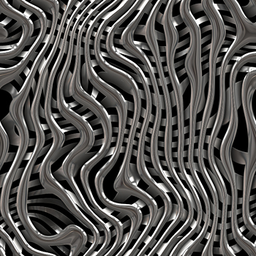
\includegraphics[width=0.5\textwidth]{assets/metal.png}
\end{center}
使用命令 \dcmd{BitmapSize} 将该图案平铺到整个 480 $\times$ 272 大小的屏幕上,可以得到以下结果: 
\png{tiled-norot}
整个结果还算尽人意,不过还是能看出很明显的重复部分。
将这个位图使用函数 \cmd{rotate}
\cmdidx{cmd\_rotate}
旋转一个奇数角度 -- 比如3333 Furmans角度,大约为18$^\circ$ --
就可以让重复的部分不显得那么突兀。

\newpage
\section{绘制阴影}
\index{shadows}
\index{drawing|shadows}
\png{0025}
为了实现阴影的效果,需要依次绘制两次图形。首先使用阴影的颜色在目标位置附近( $x$ 和 $y$ 方向上各进行一段偏移)绘制一遍图形,之后使用前景色再次绘制一遍图形。
\eg{examples-dropshadow}
这个例子使用了 3 像素的偏移值来绘制阴影,可见这种方法对较大字体比较有效。而对于小一点的字体,1 到 2 像素的偏移看上去会更好一些。

\noindent
\begin{minipage}[][][t]{0.45\textwidth}

\includegraphics[width=1.0\textwidth]{assets/logodrop.png}
\end{minipage}
\begin{minipage}[][][t]{0.55\textwidth}
同样的方法也可以用在绘制位图上:首先用黑色将原位图绘制出来,之后用正常的颜色在附近再绘制一次。左图利用这种方法绘制了Gameduino的Logo,采用了50\%的透明来起到阴影的效果。
\index{logo}
\end{minipage}

\newpage
\section{淡入与淡出}

\begin{center}
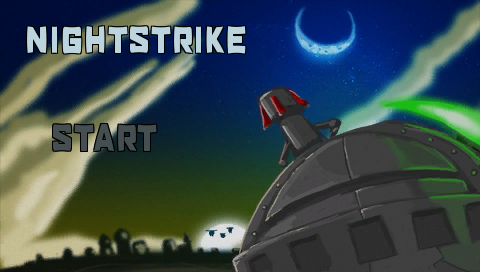
\includegraphics[width=0.3\textwidth]{fade/0.png}
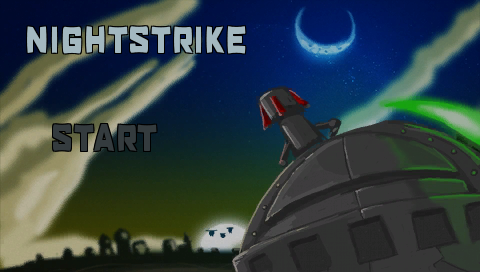
\includegraphics[width=0.3\textwidth]{fade/1.png}
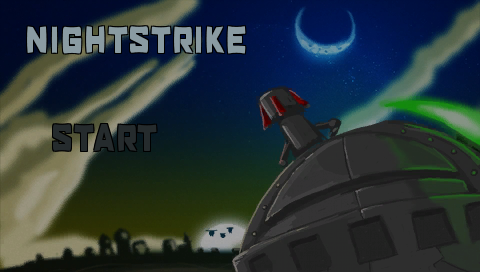
\includegraphics[width=0.3\textwidth]{fade/2.png}
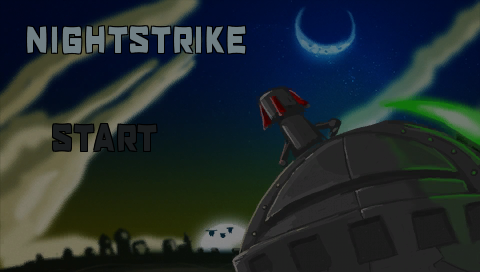
\includegraphics[width=0.3\textwidth]{fade/3.png}
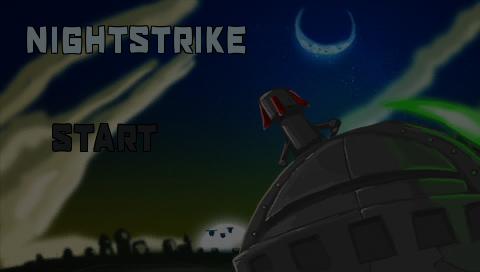
\includegraphics[width=0.3\textwidth]{fade/4.png}
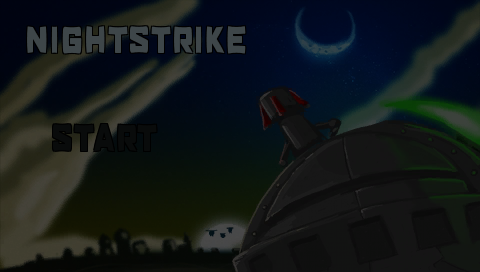
\includegraphics[width=0.3\textwidth]{fade/5.png}
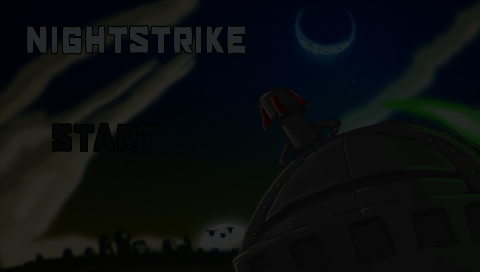
\includegraphics[width=0.3\textwidth]{fade/6.png}

\includegraphics[width=0.3\textwidth]{fade/7.png}
\includegraphics[width=0.3\textwidth]{fade/8.png}
\end{center}

\term{淡入} 是一种逐渐改变屏幕颜色的技术。淡入到黑色或者白色是最常见的两种情况,当然淡入到其他颜色也是可能的。
其中一种制造出淡入效果的方法是绘制一个屏幕大小的矩形,通过不断改变矩形的alpha值来实现过渡的效果。
于是Alpha的大小就决定了原图像有多大程度被矩形覆盖了,这样只要逐渐将alpha大小从 0 上升到 255,就可以实现场景过渡的效果。

以下是 \textit{NightStrike} 的一段代码,该代码演示了如何实现将标题画面逐渐过渡到黑色的方法。
\index{NightStrike}

\eg{nightstrike-fade}

注意一开始的 \dcmd{TagMask} 命令旨在取消写入触摸标签的缓冲。
如果没有这条命令,绘制整个屏幕的矩形将会覆盖所有已存的其他触摸标签。


\newpage
\section{动态模糊}
\index{motion blur}
\index{chess}
\index{demos!chess}
\png{chess}

动态模糊技术被用于平滑物体的运动,从而使物体的运动过程更为自然。
图中在棋盘上运动的白色棋子用动态模糊进行了渲染。
如果只从单帧上看,物体会显得很不清晰。但如果把帧与帧之间连续起来播放,
视觉系统就会把其辨认为一个快速移动的物体。

在 \gdtwo 中渲染动态模糊效果的方法之一,是在同一时间用多个不同的透明度绘制同一个物体。 
在这个 ``chess'' 的演示程序中,用于渲染的数量是由 \mach{OVERSAMPLE}变量控制的,其值被设置为 8。
渲染器按照采样数量同时绘制多次图形,每一个图形之间存在细微的距离差。
如此一来,8 个彼此叠加的透明部分就在运动路径上产生了模糊的视觉效果。

\eg{chess-a}

\newpage
\section{叠加混合}
\index{blending}

\begin{center}
\includegraphics[width=0.55\textwidth]{assets/0048.png}
\includegraphics[width=0.55\textwidth]{assets/0049.png}
\end{center}
 
以上两个图片都是由下方的代码完成的。
这段代码绘制了 1000 个直径为 8 像素的圆形,在绘制时使用了 \dcmd{BlendFunc} 函数。
该函数设置了将每个像素的颜色与背景的颜色进行叠加。
这两幅图的区别在于,顶上的图片使用的颜色为纯绿色 (\mach{0x00ff00})
而底部使用的是一个稍浅的绿色(\mach{0x60c030})。

对于纯绿色来说,任何多次绘制的图形依然是绿色的。
而对于浅绿色来说 \mach{0x60c030} -- 包含了绿色,红色和少量蓝色 --, 每一次叠加绘制都会让颜色更为明亮一些。
不过在这种情况下,同一个像素被绘制 6 次之后就会变成纯白色 \mach{0xffffff},此后就无法变得更亮了。

\eg{examples-additive}

\newpage
\section{高效率的矩形绘制}
\index{drawing!rectangles}
\png{0052}
这段代码首先设置了一个大小为 1$\times$1 像素的 \mach{L8} 位图。
混合函数 \mach{(ONE, ZERO)} 仅仅是一个直接替换操作:像素从位图中拷出,被复制到颜色缓冲中。
% The source address for the bitmap is set to \mach{ROM\_PIXEL\_FF}, which is an address in the GPU's ROM that has value 255.
对一个 \mach{L8} 位图而言,RGB像素的值就是其当前的颜色。

之后的代码将位图的绘制大小设置为了60$\times$30 像素。
这个意味着 60$\times$30 大小的位图都会被当前颜色覆盖。
这样的话,每次使用 vertex 绘制的时候都会是一个实心矩形了。

使用这种方式绘制的矩形在多个方面有别于使用 \mach{RECTS} 绘制。
首先,这些矩形没有反走样的功能:它们的大小完完全全是 60$\times$30,而没有任何的边缘平滑处理。
第二个不同之处在于,此处每一个 \dcmd{Vertex2ii} 都将绘制一个矩形;
而在 \mach{RECTS} 中,每一个矩形需要调用两次vertex。
\eg{examples-1x1}

\newpage
\section{一维位图}
\index{bitmaps!1D}
\png{0053}

\eg{examples-1d}

这段代码使用了以下的 512$\times$1 像素的``光谱'' 图像。这个图像作为一个\mach{RGB565} 位图被载入到图形缓存中。
\begin{center}
\includegraphics[width=1.0\textwidth]{assets/spectrum.png}
\end{center}

\noindent
\dcmd{BitmapSize} 指令配合 \mach{REPEAT} 参数可以将位图进行平铺。
由于位图的高度是一个像素,它在每一行都进行了重复。
\index{bitmaps!tiling}
% \eg{examples-1d-twist}
我们知道对于任何一个一维位图来说,都可以对其进行伸缩和旋转。以下就是同一个位图经过 0.3 倍的伸缩与 80$^\circ$  旋转之后得到的结果。

\begin{center}
\includegraphics[width=0.5\textwidth]{assets/0054.png}
\end{center}

\newpage
\section{多边形绘制}
\index{drawing!polygons}

\png{0050}

GD图形库有一个专门用于绘制多边形的辅助对象 \textit{Poly}。
如果需要绘制一个多边形,首先需要调用 \mach{begin()} 方法,
之后再将多边形的顶点按照子像素坐标依次传递给 \mach{v()} 方法。
最后使用 \mach{draw()} 用当前颜色完成多边形的绘制。

例程中只使用了 4 个顶点,但实际上多边形最多可以支持 16 个顶点。
多边形可以是任何形状,并且顶点不一定都需要在屏幕可见范围。

\mach{Poly} 对象使用了一系列的模板缓冲操作来计算多边形的轮廓。
最后它使用当前颜色和Alpha值设置填充多边形的内部,整个过程和 \mach{POINTS} 或者 \mach{LINES} 十分类似。

\eg{examples-polygon}

\newpage
但是和 \mach{POINTS} 或者 \mach{LINES} 方法不同,多边形并没有对边缘进行平滑处理。这导致了多边形的边缘上会出现锯齿。
解决方法之一就是在多边形的边缘上再次勾勒直线边缘。
此处利用\mach{Poly} 对象的方法 \mach{outline()},一个宽黑色边缘通过
\mach{LINE\_STRIP} 方法绘制了出来。

\eg{examples-polygon2}

\png{0051}

\index{demos!cobra}
例程 \textit{cobra} 使用了类似的方法,首先用 \mach{Poly} 绘制了多边形,
之后又勾勒了微微发光的蓝色外边界。
\index{edges}
\png{cobra}

\newpage
\section{无所不在的直线}
\index{lines}

因为直线顶端有宽圆角的存在,宽直线可以作为非常实用的图形元素存在。
在例程 \textit{sprites} 中,一个宽 28 像素、Alpha 50\%的黑色宽直线就被用于绘制了文本框的背景。
\png{lines-el}
\eg{sprites-line}

\textit{NightStrike} 程序中在画面顶端使用了三个水平放置的宽直线来绘制能量槽。
\index{NightStrike}
首先一个 $10$ 像素的浅黑色长条作为能量条的背景,而当前能量的指示由两条直线配合完成:
一条为 $10$ 像素的淡橘色,另一条为 $4$ 像素的亮橙色。这样配合下来就得到了令人满意的发光特效。
\index{glow effect}

\begin{center}
\includegraphics[width=0.28\textwidth]{assets/ns-pwr-0000.png}
\includegraphics[width=0.28\textwidth]{assets/ns-pwr-0001.png}
\includegraphics[width=0.28\textwidth]{assets/ns-pwr-0002.png}
\includegraphics[width=0.28\textwidth]{assets/ns-pwr-0003.png}
\includegraphics[width=0.28\textwidth]{assets/ns-pwr-0004.png}
\includegraphics[width=0.28\textwidth]{assets/ns-pwr-0005.png}
\includegraphics[width=0.28\textwidth]{assets/ns-pwr-0006.png}
\includegraphics[width=0.28\textwidth]{assets/ns-pwr-0007.png}
\includegraphics[width=0.28\textwidth]{assets/ns-pwr-0008.png}
\end{center}

\newpage
\section{晕映(vignetting)}
\index{photography}

\begin{center}
\includegraphics[width=0.48\textwidth]{assets/vignette-0.png}
\includegraphics[width=0.48\textwidth]{assets/vignette-1.png}
\end{center}

\term{晕映} 是在摄影中一种将图片边角暗化的技术。
上方右图中就将晕映作为了一个额外的图层。晕映图片本身是一个 480$\times$272 像素的 \mach{L8} 放射渐变图形,越至边缘透明度越低:

\begin{center}
\setlength{\fboxsep}{0pt}
\setlength{\fboxrule}{1pt}
\fbox{\includegraphics[width=0.6\textwidth]{assets/vignette.png}}
\end{center}

如果用白色绘制这个位图,边缘会得到乳白色的透明效果。而用黑色绘制该位图,则会让边缘更加暗化。暗化的程度即可以通过修改原位图控制,也可通过 \mach{ColorA} 方法改变位图的不透明度。

\eg{abstract3-vignette}

因为晕映图像自身并没有太多细节,所以降低分辨率也不会对图像质量造成很多的影响。
比如一个 240$\times$136 像素的晕映位图和一个 480$\times$272 像素的位图相比并没有太多可观的差别,但是前者只占用了后者四分之一的内存。

\newpage
\section{镜像的图元}
\label{mirror}
\index{bitmaps!mirroring}
\index{sprites}

\noindent
\png{mirror}

\textit{镜像} 一个图元,把它调整它的镜像方向上,是在2D游戏中十分有用的操作。
Gameduino 2的GPU单元可以处理复杂的位图变换,自然简单的翻转更不会存在问题。
你可以设想一个左右的翻转实际上就是x轴被乘以了-1倍,该操作用 \cmd{scale} 就可以完成。
代码中两次 \cmd{translate} 调用仅仅是修改了位图的位置,以保证翻转的中心轴在图元的中心处。
在这个例子中,图元是 $32$ 像素宽的,所以翻转是在 $x = 16$ 处完成的:

\begin{center}
\begin{tikzpicture}
  \node [opacity=0.4] {\includegraphics[scale=0.32]{previews/walk-WALK-00.png}};
    \draw [dashed,thick]   (0,-1)  -- (0,1);
\end{tikzpicture}
\end{center}

\eg{examples-mirror}

\newpage
\section{轮廓与边缘}
\index{silhouettes}
\index{drawing!silhouettes}
\index{edges}
\png{outline1}

Gameduino 2的硬件底层只支持实心圆和直线的绘制。那么如何实现上图的效果:在圆的周围勾勒出线条呢?答案非常简单 -- 绘制圆形两次。

一个稍大的圆首先用边界的颜色绘制出来,之后稍小一点的圆再使用圆内部的颜色绘制。
对于一群绘制的物体来说,绘制顺序将影响最终的图像。此处外轮廓的圆先绘制,这样可以给整个集群一个共有的边界。

% \eg{abstract3-outline}

\begin{center}
\includegraphics[width=0.48\textwidth]{assets/outline3.png}
\includegraphics[width=0.48\textwidth]{assets/outline2.png}
\end{center}

下图中按钮的边缘效果也是依靠两个直线绘制的 -- 一个白色直线和一个比它窄 $4$ 个像素的蓝色直线。

这种边缘绘制方法也可以用于
\mach{POINTS}, \mach{LINES} 和
\mach{RECTS} 中。

\begin{center}
\includegraphics[width=0.6\textwidth,trim=120 100 120 100,clip=true]{assets/0057.png}
\end{center}

\newpage
\section{粗糙的像素感}
\cmdidx{cmd\_scale}
\index{retro}
\index{Zardoz}

\png{zardoz}

对于艺术家和设计师 Nick Criscuolo 来说,他更希望用Gameduino 2的图形系统实现更加粗糙、8位像素的复古感。在 \textit{Zardoz} 项目中,所有的图形都是以两倍伸展的方式绘制的。在每一帧开始之前,都会调用以下代码来把其绘制的每个位图扩展两倍:

\eg{zardoz-double}

\noindent
这样一来的结果就是原图中的每个像素都变成了屏幕上 2$\times$2 个像素。这导致了游戏的等效分辨率变为了 240$\times$136 (Gameduino 2 的原始分辨率为 480 $\times$136)。
\index{emulating!low resolution displays}

\newpage
\section{矢量图形}
\index{vector displays}

\png{vector}

\index{drawing!vectors}

矢量图形游戏在70、80和90年代期间,因为当时特殊的硬件条件,可以在CRT显示器上绘制出明亮、彩色的矢量线条。
\index{emulating!CRT}
\index{CRT, emulating}
作为一个图形技术,这种绘制方式的优势在于不需要像素的概念:所有的一切都是由平滑明亮的直线和点构建而成的。
\gdtwo 有非常完善的平滑线条和点的绘制支持,所以可以轻易模拟出这种矢量绘图方法。

然而如果仅仅用直线来绘制游戏,恐怕看上去太“单薄”了:还需要模仿原来图形上微微发亮的效果。这个特效将分成两步实现。首先编写 \mach{drawgame()} 函数,其作用是绘制屏幕上所有的直线,之后将使用两种不同的线条属性来调用该函数进行绘制。
\defidx{LINES}
第一步的绘制中,配置直线为稍宽的尺寸,使用背景亮光的颜色来绘制所有直线,之后调用 \mach{drawgame()}。
第二步绘制的直线位置完全相同,但是在样式上使用了更为明亮,且线宽较细的直线。
这两步绘制之后,所有的直线都实现了微光的效果。
\index{glow effect}

\eg{tempest-draw}

\newpage
\section{手绘图形}
\index{handmade}
\index{weave}
\index{binary}

\begin{center}
\includegraphics[height=0.3\textwidth]{assets/weave.png}
\includegraphics[height=0.3\textwidth,trim=100 60 100 60,clip=true]{assets/0067.png}
\end{center}

早期人们并没有像我们一样复杂的设计工具,所有的图形都是首先绘于纸稿之上,最后再徒手转换成数据的。如今,你也可以试着用同样的方法设计图形。
\cmd{memwrite} 函数将 $8$ 个字节构成的图案写入在起始地址为 $0$ 的内存地址之中。
二进制编码的图案被存放在 \mach{picture[]} 中 -- ``\mach{0b}'' 前缀表示数据为二进制表示。
之后,这个程序将这个 8$\times$8 \mach{L1} 格式的位图在整个屏幕的 $x$ 和 $y$ 上平铺。

\eg{examples-handmade}

%%%%%%%%%%%%%%%%%%%%%%%%%%%%%%%%%%%%%%%%%%%%%%%%%%%%%%%%%%%%%%%%%%%%%%%%
\chapter{图形混合}

\index{compositing}
本章介绍了更为复杂的图形技术,挖掘GPU硬件的潜力。
他们无一例外的使用了合成技术 -- 使用Alpha通道控制颜色通道。

\newpage
\section{Alpha合成}

\png{comp1}

\index{drawing!clock}
这个有型的时钟是由一个白色圆圈,一个小的黑色圆圈和一个 \cmd{clock} 控件绘制的时针组成的。

\eg{examples-comp1}

但是如果你想为其添加一个JPEG格式的背景的的话,结果就却是悲剧的:

\begin{center}
\includegraphics[width=0.4\textwidth]{assets/comp2.png}
\end{center}
\newpage

黑色的大圆盘毁掉了整个设计感,如果能将中心圆盘变为透明色,整个画面感就能大幅提升。
其中之一的解决之道是使用\term{alpha缓冲}。

\index{alpha!buffer}
屏幕上每个像素都有一个0-255的alpha值,这个alpha值通常和颜色缓冲同时更新。
一般来说alpha缓冲的存在并非必要,因为它并不可见,而且不会影响最终图像。
而 \dcmd{ColorMask} 命令可以允许或禁止对颜色缓冲和alpha缓冲的写入。
这个技术首先将图形``绘制''至alpha缓冲中,之后使用 \mach{BlendFunc(DST\_ALPHA, ONE)}
实现对屏幕上所有像素的混合模式绘制。在绘制时,只有alpha缓冲非零时才会被绘制出来。

绘制完绿树的背景之后,首先用 \dcmd{ColorMask} 函数禁止对颜色缓冲写入,之后向 \dcmd{BlendFunc} 
写入一个可以把之后的alpha值直接写入alpha缓冲的参数。设置方法是将 \term{源混合因子} 设置为 \mach{ONE}:

\eg{examples-comp2a}

现在和之前一样绘制出外部圆形:

\eg{examples-comp2b}

这样之后,并没有图形真正出现在屏幕上,因为上述操作实际上只会影响alpha缓冲,目前为止还是不可见的。
绘制内部圆时需要将混合模式设置为覆盖之前已经绘制的所有像素,即将源混合因子设置为 \mach{ZERO}:

\eg{examples-comp2c}

\newpage
最后时钟控件的本体使用 \mach{ONE} 的混合因子进行了绘制:

\eg{examples-comp2d}

经过以上的操作之后,目前还没有任何内容能在屏幕上可见 -- 
因为 \dcmd{ColorMask} 命令静止了对R,G,B通道的绘制。
但是在alpha缓冲上,已经有了以下的图像:
\begin{center}
\includegraphics[width=0.8\textwidth]{assets/comp1.png}
\end{center}

最后一步就是让整个alpha缓冲变为可见,代码通过绘制一个整屏的灰色矩形实现。
当然,如果仅仅简单这么做自然不行,不同之处在于此处将源混合因子设置为了 \mach{DST\_ALPHA},
这样一来,透明值的大小就来自于alpha缓冲了。

\eg{examples-comp2e}
\png{0042}
完整的代码如下:
\eg{examples-comp2}

\newpage
\section{Slot gags}

\begin{center}
\includegraphics[width=0.32\textwidth]{assets/slotgag/00.png}
\includegraphics[width=0.32\textwidth]{assets/slotgag/02.png}
\includegraphics[width=0.32\textwidth]{assets/slotgag/04.png}
\includegraphics[width=0.32\textwidth]{assets/slotgag/06.png}
\includegraphics[width=0.32\textwidth]{assets/slotgag/08.png}
\includegraphics[width=0.32\textwidth]{assets/slotgag/10.png}
\includegraphics[width=0.32\textwidth]{assets/slotgag/12.png}
\includegraphics[width=0.32\textwidth]{assets/slotgag/14.png}
\includegraphics[width=0.32\textwidth]{assets/slotgag/16.png}
\end{center}

\term{Slot gags} 是一个非常古老用于将两个元素合成在一起的动画技术
masking two elements together\footnote{
\index{masking}
见 Steve Wright 的 ``Digital Compositing for Film and Video'' 一书。
}。
在这个slot gag的例子中,我们将Gameduino的位图logo的alpha缓冲设为了
\index{logo}
255,而将其他地方设置为0。 之后设置一个宽的对角线,并且将 \dcmd{BlendFunc} 的参数设置为 \mach{(DST\_ALPHA, ONE)}。 如此一来,alpha缓冲就会作为蒙板来绘制直线,这样只有在alpha缓冲为255
的地方才会绘制像素。最终的效果就是得到一个如图的闪光动画效果。
\index{glint effect}
\index{drawing!glint}

\eg{slotgag-a}

\newpage
\section{有图案的文本}
\index{drawing!patterned text}
\index{text, patterned}

\png{0060}

有图案的文本使用了和之前slot gags相似的技术。
首先,文本\textit{仅}在alpha缓冲中绘制。之后一个 8$\times$8 的位图图案在整个屏幕上绘制出来,
绘制的不透明度由aplha缓冲决定。

\begin{center}
\includegraphics[width=0.1\textwidth]{previews/examples2-EX2_STRIPE-00.png}
\end{center}
\eg{examples-stripe2}

\newpage
\section{Alpha操作}
\index{alpha}
\png{0063}
你可以设置一个宏操作让冗长的alpha合成函数的可读性更好。
此处, \mach{PAINT\_ALPHA()} 表示 ``在alpha缓冲中绘制'';
而 \mach{CLEAR\_ALPHA()} 则表示 ``从alpha缓冲中删除''。

\eg{examples-alpha1}

\newpage
\section{圆角图片}
\index{corners, round}
\index{round corners}
\png{0064}

上方左图是一个使用 \dcmd{Vertex2ii} 绘制的 128$\times$128 位图。
右边的图在左图的基础上增加了漂亮的圆角外边。
绘制这种图形的技巧在于,首先在alpha缓冲中绘制一个圆角矩形,之后利用这个矩形来控制位图的透明度,依然使用\dcmd{BlendFunc} 函数。
\index{RECTS}

圆角半径 \mach{r} 控制了圆角的圆滑度,单位为像素。
\mach{r} 设置为1是为方形,数值越大,圆角度也会越大。
% For batches of round-corners images, for example in a gallery or menu,
% is is a good idea to draw all the rectangles before switching to color buffer drawing
% and rendering the bitmaps themselves.
% This reduces the number of state changes required for each bitmap.

\eg{examples-corners}

\newpage
\section{透明的按钮}
\png{keypad}
这段代码首先绘制了全屏大小的背景图片,然后所有的按钮首先通过函数\mach{button()} 绘制在了alpha缓冲中。而代码的最后六行让alpha通道变为可见。
\eg{examples-keypad}

\newpage
\mach{button()} 函数首先绘制了一个白色矩形,然后是略小透明的另一个矩形。
最后使用 \cmd{number} 命令显示数字值,\mach{OPT\_CENTER} 参数将文本设置为居中显示。

\eg{examples-button}

\newpage
\section{反射}
\index{reflections}
\index{drawing!reflections}
\png{reflection0}

首先绘制好logo的位图,之后程序在alpha缓冲中绘制了一个 128$\times$1 的渐变位图,
该渐变在水平方向上重复,直到全部覆盖屏幕:

\begin{center}
\includegraphics[width=0.5\textwidth]{assets/reflection1.png}
\end{center}

之后的代码利用位图变换将logo在Y轴方向上进行了翻转,所用的技术和 \xref{mirror} 中使用的类似。
之后的代码将logo的alpha通道连同现有的alpha内容全部写入到alpha缓冲中。

蒙版的操作使用了宏 \mach{MASK\_ALPHA()}, 该宏的作用是将logo的alpha通道和现在的alpha缓冲值进行乘法操作:
\index{matte}
\index{masking, alpha}
\index{alpha!masking}

\vspace{10pt}
$\vcenter{\hbox{\includegraphics[width=0.3\textwidth]{assets/reflection1.png}}}$
$\times$
$\vcenter{\hbox{\includegraphics[width=0.3\textwidth]{assets/reflection3.png}}}$
$=$
$\vcenter{\hbox{\includegraphics[width=0.3\textwidth]{assets/reflection2.png}}}$

\newpage
最后一步是将镜像后的logo通过alpha缓冲绘制出来。

\eg{reflection-A}

%%%%%%%%%%%%%%%%%%%%%%%%%%%%%%%%%%%%%%%%%%%%%%%%%%%%%%%%%%%%%%%%%%%%%%%%
\chapter{内存的节约}

\newpage
\section{双色位图}
\png{mono}
\eg{mono-a}
此处所用的源图像来自于 Patrick Hoesly 设计的无缝纹理:
\begin{center}
\includegraphics[width=0.3\textwidth]{assets/tile_green.jpg}
\end{center}
一般情况下,这样的图片会用 \mach{RGB565} 编码。然而此处因为这张图片只使用了两种颜色,经过适当处理就可以使用
\mach{L4} 位图格式来存储,如此一来可以节约 $75\%$ 的 图形内存  
(具体图片格式与对应的内存占用情况请参见命令 \dcmd{BitmapLayout} )。
首先将原始图片载入到图片处理软件中,用色彩取样工具分别得到两个颜色的具体RGB数值。此处经过测量,深绿色为
\mach{0x375e03},而浅绿色为
\mach{0x68b203}。 
之后将位图转换为单色位图,并调整对比度,使其在纯黑与纯白之间自然过渡。
\begin{center}
\includegraphics[width=0.3\textwidth]{assets/tile_greenm.png}
\end{center}

该程序的代码首先将屏幕清除成深绿色,之后将 \mach{L4} 的位图用浅绿的颜色绘制出来。
所得到的结果和最初的图片没有太大区别,但却节约了大量的内存。
这个 128 $\times$ 128 的 \mach{L4} 位图只是用了KB的内存。

除此之外,你还可以在程序运行阶段随意调整前景色和背景色,完全按照你自己的审美标准来就行了。
\begin{center}
\includegraphics[width=0.3\textwidth]{assets/mono1.png}
\includegraphics[width=0.3\textwidth]{assets/mono2.png}
\includegraphics[width=0.3\textwidth]{assets/mono3.png}
\end{center}

\newpage
\section{潜藏的 \mach{L2} 格式}
\label{twobit}
\index{L2@\mach{L2} bitmap format, emulating}

\png{0055}

Gameduino 2的GPU支持三种单色格式: \mach{L1}, \mach{L4}和 \mach{L8}。
这里虽然没有 \mach{L2} 格式,但是通过两次绘制却可以仿真出来。
此处的技巧就是将原图片转换成两个1位 \mach{L1} 位图,其中一个存储低位,另一个存储高位:

\begin{center}
\includegraphics[width=0.35\textwidth]{assets/abe1.png}
\includegraphics[width=0.35\textwidth]{assets/abe0.png}
\end{center}

以上名为 \mach{ABE} 图片被载入到了位图单元0和1中,位图的句柄为 \mach{ABE\_HANDLE}。 
位图单元0中存储位0,位图单元1中存储位1。
代码总共绘制了三次图片。前两次分别将两个位图载入到alpha缓冲中,而第三次操作将alpha缓冲变为可见。

绘制代码首先使用 \dcmd{ColorMask} 禁用了颜色缓冲的写入。
之后将高位用alpha值 \mach{0xaa} 表示,而低位则用 \mach{0x55} 表示。
这就得到了alpha值和2位像素之间的转换关系:

\begin{center}
\begin{tabular}{ccc}
高位 & 低位 & alpha值 \\
\hline
0 & 0 & \mach{0x00} \\
0 & 1 & \mach{0x55} \\
1 & 0 & \mach{0xaa} \\
1 & 1 & \mach{0xff} \\
\end{tabular}
\end{center}

\eg{examples-2bit}

最后的 \dcmd{Vertex2ii} 和之前两个绘制指令绘制的图形完全相同,但是由于 \dcmd{BlendFunc} 的参数设置成为了\mach{(DST\_ALPHA, ONE\_MINUS\_DST\_ALPHA)},图片的原始像素全部被忽略了,取而代之的仅仅是alpha缓冲中的像素会影响最终的颜色内容。

\newpage
\section{分离的形板(matte)}
\index{bitmaps!mattes}
\label{mattes}

\png{nightstrike_1-DEFENSOR_FRONT-00}

\textit{NightStrike}
\index{NightStrike}
游戏中所使用的基座是一个包含alpha通道的单色位图。
硬件系统中并没有办法直接支持单色含alpha通道的位图格式,但是可以通过将原始位图分离成一个
\term{形板(matte)}
来解决。其中一个是原来的alpha通道,另一个是前景图片。

\begin{center}
\includegraphics[width=0.4\textwidth]{previews/nightstrike_1-DEFENSOR_FRONT-00.png}
\includegraphics[width=0.4\textwidth]{previews/nightstrike_1-DEFENSOR_FRONT-01.png}
\end{center}

以上两个位图都以 \mach{L4} 格式被载入系统/
形板位图首先被绘制出来,绘制时将 \dcmd{ColorRGB} 设置为黑色。
这个操作将所有被形板覆盖的区域清空,之后前景图片按照通常的方法被绘制。
\begin{center}
\includegraphics[width=0.3\textwidth]{assets/ns-matteA-0000.png}
\includegraphics[width=0.3\textwidth]{assets/ns-matteB-0000.png}
\end{center}

\newpage
\section{减半分辨率}
\index{bitmaps!half-resolution}

在 \textit{NightStrike} 游戏中,直升机的动画使用了两帧100像素宽的 \mach{RGBA4} 图片:
\index{NightStrike}

\begin{center}
\includegraphics[width=150pt]{previews/nightstrike_1-HELI-00.png}
\includegraphics[width=150pt]{previews/nightstrike_1-HELI-01.png}
\end{center}

而直升机从空中坠落到地面的过程则使用了另外一个四帧的动画。因为下落的过程很快,这个动画只是转瞬即逝,一些细节上的损失并不会引起用户的注意。
所以在这个动画中使用的分辨率只有之前的一半:小于50像素。在屏幕上显示之前,只要用 \cmd{scale} 将该位图缩放到同样的尺寸就可以了。
使用这种方法减半分辨率,可以节约75\%的内存使用量。

\begin{center}
\includegraphics[width=135pt]{previews/nightstrike_1-COPTER_FALL-00.png}
\includegraphics[width=135pt]{previews/nightstrike_1-COPTER_FALL-01.png}
\includegraphics[width=135pt]{previews/nightstrike_1-COPTER_FALL-02.png}
\includegraphics[width=135pt]{previews/nightstrike_1-COPTER_FALL-03.png}
\end{center}

\newpage
\section{8位图片格式}
\label{eightbit}

\begin{center}
\includegraphics[width=0.6\textwidth]{assets/0034.png}
\end{center}

对于大部分图片来说,16位的位图格式如
\mach{RGB565},
\mach{ARGB1555} 和
\mach{ARGB4} 才是合适的。
但有时8位位图可以替代它们,在起到同样的效果的情况下不会产生明显的失真。

上图中的纸牌就是用 \mach{RGB332} 格式编码的,每个像素仅占用1个字节(8位)。
而下图中的爆炸动画则使用了 \mach{ARGB2} 格式。
\index{playing cards}
\index{cards}
对于纸牌来说,其用了大胆鲜明的颜色搭配,所以将颜色下降到 \mach{RGB332} 并不会引人注意;
而对于爆炸动画来说,因为整个过程只有0.25秒的时间,快速的动作掩饰掉了颜色范围的缺失。
\index{explosion}
\index{animation}

\begin{center}
\includegraphics[width=0.19\textwidth]{previews/nightstrike_1-FIRE-00.png}
\includegraphics[width=0.19\textwidth]{previews/nightstrike_1-FIRE-01.png}
\includegraphics[width=0.19\textwidth]{previews/nightstrike_1-FIRE-02.png}
\includegraphics[width=0.19\textwidth]{previews/nightstrike_1-FIRE-03.png}
\includegraphics[width=0.19\textwidth]{previews/nightstrike_1-FIRE-04.png}
\includegraphics[width=0.19\textwidth]{previews/nightstrike_1-FIRE-05.png}
\includegraphics[width=0.19\textwidth]{previews/nightstrike_1-FIRE-06.png}
\includegraphics[width=0.19\textwidth]{previews/nightstrike_1-FIRE-07.png}
\includegraphics[width=0.19\textwidth]{previews/nightstrike_1-FIRE-08.png}
\includegraphics[width=0.19\textwidth]{previews/nightstrike_1-FIRE-09.png}
\includegraphics[width=0.19\textwidth]{previews/nightstrike_1-FIRE-10.png}
\includegraphics[width=0.19\textwidth]{previews/nightstrike_1-FIRE-11.png}
\includegraphics[width=0.19\textwidth]{previews/nightstrike_1-FIRE-12.png}
\includegraphics[width=0.19\textwidth]{previews/nightstrike_1-FIRE-13.png}
\includegraphics[width=0.19\textwidth]{previews/nightstrike_1-FIRE-14.png}
\end{center}
\clearpage

\newpage
\section{DXT1}
\label{dxt1}
\index{DXT1}

\begin{center}
\includegraphics[width=0.48\textwidth]{assets/nightstrike/backgrounds/welcome.jpg}
\includegraphics[width=0.48\textwidth]{assets/dxt1.png}
\end{center}

DXT 是一个贴图压缩系统,它将较大的图片压缩成为更小的位图从而节约图形内存。
左方的截图是由原艺术家设计、渲染的 \textit{NightStrike} 欢迎界面,而在右边是在Gameduino2上实际运行着的,并经过DXT1压缩后的版本。
两幅图片用肉眼难分差别,但是用DXT1压缩后的图片只使用了原始大小四分之一的内存。

总体上来说,DXT1的工作原理是将原始图片分割成 4$\times$4 像素的区域。每一个区域被赋予两种颜色,名曰 $C_0$ 和 $C_1$。
之后区域内的每个像素都被表示成 $C_0$ 和 $C_1$ 的混合值。
DXT1 使用 \mach{RGB565} 格式表示颜色 $C_0$ 和 $C_1$,而对每个像素使用两位的编码:

\vspace{10pt}
\begin{tabular}{cl}
编码 & 颜色 \\
\hline \\
00 & $C_0$ \\
01 & $0.666 \times C_0 + 0.333 \times C_1$ \\
10 & $0.333 \times C_0 + 0.666 \times C_1$ \\
11 & $C_1$ \\
\end{tabular}
\vspace{10pt}

\noindent
如此一来,每个 4$\times$4 单元所占用的位大小就是:

\vspace{10pt}
\begin{tabular}{cl}
$C_0$ & 16 \\
$C_1$ & 16 \\
像素点 & 16 $\times$ 2 = 32 \\
\end{tabular}
\vspace{10pt}

计算得知每一个区域单元占用的大小为64位,因为一个单元中有16个像素点,平均下来每一个像素点所占用的内存仅为4位。
设想如果这个位图是用 \mach{RGB565} 编码的,那么每个像素将占用16位,用DXT1压缩可以节约75\%的图形内存!

可惜的是Gameduino 2的硬件并不直接支持DXT1,但是通过多次绘制和相乘的方法可以将其模拟出来。

\clearpage

以 \textit{NightStrike} 的欢迎界面为例,源图片的大小为 480$\times$272 像素。
因为DXT1以 4$\times$4 大小为一个单元,于是整个图像为 120$\times$68 单元。
将所有单元的 $C_0$ 和 $C_1$ 分别保存在两个大小为 120$\times$68 像素、编码为\mach{RGB565}的图片中:

\vspace{10pt}
$C_0=$
$\vcenter{\hbox{\includegraphics[width=0.9\textwidth]{previews/nightstrike_welcome-WELCOME_BACKGROUND_COLOR-00.png}}}$

$C_1=$
$\vcenter{\hbox{\includegraphics[width=0.9\textwidth]{previews/nightstrike_welcome-WELCOME_BACKGROUND_COLOR-01.png}}}$

\newpage
因为硬件缺乏对两位图片的支持,两位的编码位图被拆分为两张一位编码的图片,具体作法见 \xref{twobit} 。

$b_0=$
$\vcenter{\hbox{\includegraphics[width=0.32\textwidth]{previews/nightstrike_welcome-WELCOME_BACKGROUND_BITS-00.png}}}$
$\;\;\;\;\;\;b_1=$
$\vcenter{\hbox{\includegraphics[width=0.32\textwidth]{previews/nightstrike_welcome-WELCOME_BACKGROUND_BITS-01.png}}}$
\vspace{10pt}

\noindent
\textit{NightStrike} DXT1 的背景绘制函数首先在alpha缓冲中构建了二位的位图,之后再将 $C_0$ 和 $C_1$位图使用 \cmd{scale} 命令放大4位并写入颜色缓冲中,最终将其与alpha缓冲的内容进行了混合。

\eg{nightstrike-dxt1}

%%%%%%%%%%%%%%%%%%%%%%%%%%%%%%%%%%%%%%%%%%%%%%%%%%%%%%%%%%%%%%%%%%%%%%%%
% \chapter{Useful things}
% \section{Light switch}
% \section{Kitchen timer}
% \section{Photo frame}

\chapter{游戏及演示程序}

\newpage
\section{Kenney}

\png{kenney}

\textit{kenney} 演示程序使用了艺术家 Kenney.nl
\footnote{\url{http://www.kenney.nl/}}
的开放艺术作品\footnote{\url{http://opengameart.org/content/platformer-art-deluxe}}。
整个程序绘制了六个图层,可以以60Hz的速度流畅运行。
其中大部分的图形都是以位图的方式绘制的,所有的位图都是以 \mach{ARGB4} 编码的。
第一层是一个垂直方向的渐变,精心挑选了天空蓝作为颜色。

\png{kenney_0}
\eg{kenney-gradient}

\noindent
下一个图层使用了一个云朵图元,这个图元被保存在 \mach{CLOUD\_HANDLE} 中。这些云朵的初始位置是随机的,位置信息保存在 \mach{state.clouds[]} 中。
所有的云朵以不同的速度向下方运动,速度越慢的云朵越透明。
当云朵到达屏幕顶部之后,它们重新从屏幕上方卷动出现。
云朵的位置是以1/16像素为单位的子像素坐标表示的,使用精确的位置可以保证云朵不会在像素之间``跳动''。

\szpng{0.2}{previews/kenney-CLOUD-00}
\png{kenney_1}
\eg{kenney-clouds}


% \szpng{0.15}{kenney_tiles}
\sbs{kenney_tiles}{
下一个图层是网格地图,网格地图是由网格编辑器生成的 (\url{http://www.mapeditor.org/})。
这个地图之后通过元素转换器被写入字符数组 \mach{layer1\_map}。
20个平铺网格单元每一个都是 32$\times$32 \mach{ARGB4} 编码的位图,句柄保存在 \mach{TILES\_HANDLE}。
平铺单元位置0处是一个空白单元,程序会检查这一点并且只绘制非0单元。
\szpng{1.0}{assets/kenney_2}
}
\begin{center}
\includegraphics[width=0.09\textwidth]{previews/kenney-TILES-00.png}
\includegraphics[width=0.09\textwidth]{previews/kenney-TILES-01.png}
\includegraphics[width=0.09\textwidth]{previews/kenney-TILES-02.png}
\includegraphics[width=0.09\textwidth]{previews/kenney-TILES-03.png}
\includegraphics[width=0.09\textwidth]{previews/kenney-TILES-04.png}
\includegraphics[width=0.09\textwidth]{previews/kenney-TILES-05.png}
\includegraphics[width=0.09\textwidth]{previews/kenney-TILES-06.png}
\includegraphics[width=0.09\textwidth]{previews/kenney-TILES-07.png}
\includegraphics[width=0.09\textwidth]{previews/kenney-TILES-08.png}
\includegraphics[width=0.09\textwidth]{previews/kenney-TILES-09.png}
\includegraphics[width=0.09\textwidth]{previews/kenney-TILES-10.png}
\includegraphics[width=0.09\textwidth]{previews/kenney-TILES-11.png}
\includegraphics[width=0.09\textwidth]{previews/kenney-TILES-12.png}
\includegraphics[width=0.09\textwidth]{previews/kenney-TILES-13.png}
\includegraphics[width=0.09\textwidth]{previews/kenney-TILES-14.png}
\includegraphics[width=0.09\textwidth]{previews/kenney-TILES-15.png}
\includegraphics[width=0.09\textwidth]{previews/kenney-TILES-16.png}
\includegraphics[width=0.09\textwidth]{previews/kenney-TILES-17.png}
\includegraphics[width=0.09\textwidth]{previews/kenney-TILES-18.png}
\includegraphics[width=0.09\textwidth]{previews/kenney-TILES-19.png}
\end{center}
\eg{kenney-tiles}

\newpage
在前景中的角色是 \mach{ARGB4} 的位图,以正弦路径运动并随机旋转。
它们的坐标值被保存在 \mach{state.p} 中。
\begin{center}
\includegraphics[width=0.2\textwidth]{previews/kenney-PLAYER1-00.png}
\includegraphics[width=0.2\textwidth]{previews/kenney-PLAYER1-01.png}
\includegraphics[width=0.2\textwidth]{previews/kenney-PLAYER1-02.png}
\end{center}
跟随角色的彩色``泡泡''是透明的 \mach{POINT} , 在代码中由三个 \mach{state.trail} 对象管理。
\png{kenney_3}
\eg{kenney-player}

``阳光普照''的图形是在云朵图层和天空的图层之间绘制的。
通过使用一系列蒙版操作实现了射线状物体的绘制。
函数 \mach{burst()} 绘制了整个阳光普照,而函数
\mach{sunrise()} 绘制了黄色和橘色的 \mach{burst()}, 并且将它们跳跃的扩展做成动画效果。

\png{kenney_4}

最后一个图层是从天而降的爱心雨,这部分的处理方法和处理云所在的图层基本相似。
数组 \mach{state.hearts[]} 记录爱心的位置,当它们落入到屏幕底部时,会从顶部卷动出现。
\szpng{0.2}{previews/kenney-HEART-00}

\png{kenney_5}

\newpage
\section{NightStrike}
\label{nightstrike}
\index{NightStrike|boldindex}

\png{nightstrike}

\textit{NightStrike} 的游戏素材来自艺术家 MindChamber 的开放艺术作品 \footnote{\url{http://opengameart.org/content/nightstrike-png-assets}}。
这个游戏使用触屏操作追踪大量的移动物体,游戏可以流畅运行在60Hz。
游戏运用了很多技巧使其适应图形系统仅有的${256}$ KB内存。
整个游戏共有五个关卡,每一个关卡都有一个独立的元素文件。这个文件保存了对应关卡所有需要的前景、背景图片以及音效内容。
每关卡的背景都是 480$\times$272 的图片,使用类似DXT1的压缩编码 (\xref{dxt1}),使其仅占用65 KB的图形缓存。

\begin{center}
\includegraphics[width=0.3\textwidth]{assets/nightstrike/backgrounds/welcome.jpg}
\includegraphics[width=0.3\textwidth]{assets/nightstrike/backgrounds/burningwoods.jpg}
\includegraphics[width=0.3\textwidth]{assets/nightstrike/backgrounds/greenland.jpg}
\includegraphics[width=0.3\textwidth]{assets/nightstrike/backgrounds/nightfall.jpg}
\includegraphics[width=0.3\textwidth]{assets/nightstrike/backgrounds/purplesnow.jpg}
\includegraphics[width=0.3\textwidth]{assets/nightstrike/backgrounds/redworld.jpg}
\end{center}

\newpage

游戏中的图元有很平滑的透明处理,所以大部分都是以 \mach{ARGB4} 格式编码的。

\begin{center}
\includegraphics[width=150pt]{previews/nightstrike_1-HELI-00.png}
\includegraphics[width=150pt]{previews/nightstrike_1-HELI-01.png}
\end{center}

\begin{center}
\includegraphics[width=0.07\textwidth]{previews/nightstrike_0-MISSILE_A-00.png}
\includegraphics[width=0.07\textwidth]{previews/nightstrike_0-MISSILE_C-00.png}
\end{center}

\begin{center}
\includegraphics[width=0.1\textwidth]{previews/nightstrike_0-SOLDIER_RUN-00.png}
\includegraphics[width=0.1\textwidth]{previews/nightstrike_0-SOLDIER_RUN-01.png}
\includegraphics[width=0.1\textwidth]{previews/nightstrike_0-SOLDIER_RUN-02.png}
\includegraphics[width=0.1\textwidth]{previews/nightstrike_0-SOLDIER_RUN-03.png}
\includegraphics[width=0.1\textwidth]{previews/nightstrike_0-SOLDIER_RUN-04.png}
\includegraphics[width=0.1\textwidth]{previews/nightstrike_0-SOLDIER_RUN-05.png}
\includegraphics[width=0.1\textwidth]{previews/nightstrike_0-SOLDIER_RUN-06.png}
\includegraphics[width=0.1\textwidth]{previews/nightstrike_0-SOLDIER_RUN-07.png}
\end{center}

爆炸的动画快速且有明亮的颜色,所以可以使用 \mach{ARGB2} 格式节约内存 (见\xref{eightbit})。

\begin{center}
\includegraphics[width=0.18\textwidth]{previews/nightstrike_0-EXPLODE_BIG-00.png}
\includegraphics[width=0.18\textwidth]{previews/nightstrike_0-EXPLODE_BIG-01.png}
\includegraphics[width=0.18\textwidth]{previews/nightstrike_0-EXPLODE_BIG-02.png}
\includegraphics[width=0.18\textwidth]{previews/nightstrike_0-EXPLODE_BIG-03.png}
\includegraphics[width=0.18\textwidth]{previews/nightstrike_0-EXPLODE_BIG-04.png}
\includegraphics[width=0.18\textwidth]{previews/nightstrike_0-EXPLODE_BIG-05.png}
\includegraphics[width=0.18\textwidth]{previews/nightstrike_0-EXPLODE_BIG-06.png}
\includegraphics[width=0.18\textwidth]{previews/nightstrike_0-EXPLODE_BIG-07.png}
\includegraphics[width=0.18\textwidth]{previews/nightstrike_0-EXPLODE_BIG-08.png}
\includegraphics[width=0.18\textwidth]{previews/nightstrike_0-EXPLODE_BIG-09.png}
\end{center}

玩家的``炮台''是黑白的,所以用了两个 \mach{L4} 位图存储 (见\xref{mattes})。

\begin{center}
\includegraphics[width=0.4\textwidth]{previews/nightstrike_1-DEFENSOR_FRONT-00.png}
\includegraphics[width=0.4\textwidth]{previews/nightstrike_1-DEFENSOR_FRONT-01.png}
\end{center}

\newpage

除了使用运动的位图来实现爆炸效果,游戏还使用了宽线条来模拟爆炸的火花 (见\xref{lines})。
因为它们仅仅使用 \mach{LINES} 功能,所以这些火花不需要使用任何图形缓存。
\begin{center}
\includegraphics[width=0.3\textwidth]{assets/ns-lines-0006.png}
\includegraphics[width=0.3\textwidth]{assets/ns-lines-0007.png}
\includegraphics[width=0.3\textwidth]{assets/ns-lines-0008.png}
\includegraphics[width=0.3\textwidth]{assets/ns-lines-0009.png}
\includegraphics[width=0.3\textwidth]{assets/ns-lines-0010.png}
\includegraphics[width=0.3\textwidth]{assets/ns-lines-0011.png}
\end{center}

\noindent
游戏中的所有文字使用了12$\times$19像素的字体,该字体库由原始的TrueType字体转换而来。
字体的位图保存为 \mach{L4} 格式从而保存平滑的边缘过渡。

\begin{center}
\includegraphics[width=0.04\textwidth]{previews/nightstrike_2-INFOFONT-00.png}
\includegraphics[width=0.04\textwidth]{previews/nightstrike_2-INFOFONT-01.png}
\includegraphics[width=0.04\textwidth]{previews/nightstrike_2-INFOFONT-02.png}
\includegraphics[width=0.04\textwidth]{previews/nightstrike_2-INFOFONT-03.png}
\includegraphics[width=0.04\textwidth]{previews/nightstrike_2-INFOFONT-04.png}
\includegraphics[width=0.04\textwidth]{previews/nightstrike_2-INFOFONT-05.png}
\includegraphics[width=0.04\textwidth]{previews/nightstrike_2-INFOFONT-06.png}
\includegraphics[width=0.04\textwidth]{previews/nightstrike_2-INFOFONT-07.png}
\includegraphics[width=0.04\textwidth]{previews/nightstrike_2-INFOFONT-10.png}
\includegraphics[width=0.04\textwidth]{previews/nightstrike_2-INFOFONT-11.png}
\includegraphics[width=0.04\textwidth]{previews/nightstrike_2-INFOFONT-12.png}
\includegraphics[width=0.04\textwidth]{previews/nightstrike_2-INFOFONT-13.png}
\includegraphics[width=0.04\textwidth]{previews/nightstrike_2-INFOFONT-14.png}
\includegraphics[width=0.04\textwidth]{previews/nightstrike_2-INFOFONT-15.png}
\includegraphics[width=0.04\textwidth]{previews/nightstrike_2-INFOFONT-16.png}
\includegraphics[width=0.04\textwidth]{previews/nightstrike_2-INFOFONT-17.png}
\includegraphics[width=0.04\textwidth]{previews/nightstrike_2-INFOFONT-20.png}
\includegraphics[width=0.04\textwidth]{previews/nightstrike_2-INFOFONT-21.png}
\includegraphics[width=0.04\textwidth]{previews/nightstrike_2-INFOFONT-22.png}
\includegraphics[width=0.04\textwidth]{previews/nightstrike_2-INFOFONT-23.png}
\includegraphics[width=0.04\textwidth]{previews/nightstrike_2-INFOFONT-24.png}
\includegraphics[width=0.04\textwidth]{previews/nightstrike_2-INFOFONT-25.png}
\includegraphics[width=0.04\textwidth]{previews/nightstrike_2-INFOFONT-26.png}
\includegraphics[width=0.04\textwidth]{previews/nightstrike_2-INFOFONT-27.png}
\includegraphics[width=0.04\textwidth]{previews/nightstrike_2-INFOFONT-28.png}
\includegraphics[width=0.04\textwidth]{previews/nightstrike_2-INFOFONT-29.png}
\includegraphics[width=0.04\textwidth]{previews/nightstrike_2-INFOFONT-30.png}
\includegraphics[width=0.04\textwidth]{previews/nightstrike_2-INFOFONT-31.png}
\includegraphics[width=0.04\textwidth]{previews/nightstrike_2-INFOFONT-32.png}
\includegraphics[width=0.04\textwidth]{previews/nightstrike_2-INFOFONT-33.png}
\includegraphics[width=0.04\textwidth]{previews/nightstrike_2-INFOFONT-34.png}
\includegraphics[width=0.04\textwidth]{previews/nightstrike_2-INFOFONT-35.png}
\includegraphics[width=0.04\textwidth]{previews/nightstrike_2-INFOFONT-36.png}
\includegraphics[width=0.04\textwidth]{previews/nightstrike_2-INFOFONT-37.png}
\includegraphics[width=0.04\textwidth]{previews/nightstrike_2-INFOFONT-38.png}
\includegraphics[width=0.04\textwidth]{previews/nightstrike_2-INFOFONT-39.png}
\includegraphics[width=0.04\textwidth]{previews/nightstrike_2-INFOFONT-40.png}
\includegraphics[width=0.04\textwidth]{previews/nightstrike_2-INFOFONT-41.png}
\includegraphics[width=0.04\textwidth]{previews/nightstrike_2-INFOFONT-42.png}
\includegraphics[width=0.04\textwidth]{previews/nightstrike_2-INFOFONT-43.png}
\includegraphics[width=0.04\textwidth]{previews/nightstrike_2-INFOFONT-44.png}
\includegraphics[width=0.04\textwidth]{previews/nightstrike_2-INFOFONT-45.png}
\includegraphics[width=0.04\textwidth]{previews/nightstrike_2-INFOFONT-46.png}
\includegraphics[width=0.04\textwidth]{previews/nightstrike_2-INFOFONT-47.png}
\includegraphics[width=0.04\textwidth]{previews/nightstrike_2-INFOFONT-48.png}
\includegraphics[width=0.04\textwidth]{previews/nightstrike_2-INFOFONT-49.png}
\includegraphics[width=0.04\textwidth]{previews/nightstrike_2-INFOFONT-50.png}
\includegraphics[width=0.04\textwidth]{previews/nightstrike_2-INFOFONT-51.png}
\includegraphics[width=0.04\textwidth]{previews/nightstrike_2-INFOFONT-52.png}
\includegraphics[width=0.04\textwidth]{previews/nightstrike_2-INFOFONT-53.png}
\includegraphics[width=0.04\textwidth]{previews/nightstrike_2-INFOFONT-54.png}
\includegraphics[width=0.04\textwidth]{previews/nightstrike_2-INFOFONT-55.png}
\includegraphics[width=0.04\textwidth]{previews/nightstrike_2-INFOFONT-56.png}
\includegraphics[width=0.04\textwidth]{previews/nightstrike_2-INFOFONT-57.png}
\includegraphics[width=0.04\textwidth]{previews/nightstrike_2-INFOFONT-58.png}
\includegraphics[width=0.04\textwidth]{previews/nightstrike_2-INFOFONT-59.png}
\includegraphics[width=0.04\textwidth]{previews/nightstrike_2-INFOFONT-60.png}
\includegraphics[width=0.04\textwidth]{previews/nightstrike_2-INFOFONT-61.png}
\includegraphics[width=0.04\textwidth]{previews/nightstrike_2-INFOFONT-62.png}
\includegraphics[width=0.04\textwidth]{previews/nightstrike_2-INFOFONT-63.png}
\includegraphics[width=0.04\textwidth]{previews/nightstrike_2-INFOFONT-64.png}
\includegraphics[width=0.04\textwidth]{previews/nightstrike_2-INFOFONT-65.png}
\includegraphics[width=0.04\textwidth]{previews/nightstrike_2-INFOFONT-66.png}
\includegraphics[width=0.04\textwidth]{previews/nightstrike_2-INFOFONT-67.png}
\includegraphics[width=0.04\textwidth]{previews/nightstrike_2-INFOFONT-68.png}
\includegraphics[width=0.04\textwidth]{previews/nightstrike_2-INFOFONT-69.png}
\includegraphics[width=0.04\textwidth]{previews/nightstrike_2-INFOFONT-70.png}
\includegraphics[width=0.04\textwidth]{previews/nightstrike_2-INFOFONT-71.png}
\includegraphics[width=0.04\textwidth]{previews/nightstrike_2-INFOFONT-72.png}
\includegraphics[width=0.04\textwidth]{previews/nightstrike_2-INFOFONT-73.png}
\includegraphics[width=0.04\textwidth]{previews/nightstrike_2-INFOFONT-74.png}
\includegraphics[width=0.04\textwidth]{previews/nightstrike_2-INFOFONT-75.png}
\includegraphics[width=0.04\textwidth]{previews/nightstrike_2-INFOFONT-76.png}
\includegraphics[width=0.04\textwidth]{previews/nightstrike_2-INFOFONT-77.png}
\includegraphics[width=0.04\textwidth]{previews/nightstrike_2-INFOFONT-78.png}
\includegraphics[width=0.04\textwidth]{previews/nightstrike_2-INFOFONT-79.png}
\includegraphics[width=0.04\textwidth]{previews/nightstrike_2-INFOFONT-80.png}
\includegraphics[width=0.04\textwidth]{previews/nightstrike_2-INFOFONT-81.png}
\includegraphics[width=0.04\textwidth]{previews/nightstrike_2-INFOFONT-82.png}
\includegraphics[width=0.04\textwidth]{previews/nightstrike_2-INFOFONT-83.png}
\includegraphics[width=0.04\textwidth]{previews/nightstrike_2-INFOFONT-84.png}
\includegraphics[width=0.04\textwidth]{previews/nightstrike_2-INFOFONT-85.png}
\includegraphics[width=0.04\textwidth]{previews/nightstrike_2-INFOFONT-86.png}
\includegraphics[width=0.04\textwidth]{previews/nightstrike_2-INFOFONT-87.png}
\includegraphics[width=0.04\textwidth]{previews/nightstrike_2-INFOFONT-88.png}
\includegraphics[width=0.04\textwidth]{previews/nightstrike_2-INFOFONT-89.png}
\includegraphics[width=0.04\textwidth]{previews/nightstrike_2-INFOFONT-90.png}
\includegraphics[width=0.04\textwidth]{previews/nightstrike_2-INFOFONT-91.png}
\includegraphics[width=0.04\textwidth]{previews/nightstrike_2-INFOFONT-92.png}
\includegraphics[width=0.04\textwidth]{previews/nightstrike_2-INFOFONT-93.png}
\includegraphics[width=0.04\textwidth]{previews/nightstrike_2-INFOFONT-94.png}
\end{center}

游戏代码中对每一个可见物体设立了一个类对象进行管理,这些类包括:
\mach{Fires},
\mach{Explosions},
\mach{Sparks},
\mach{SoldierObject},
\mach{MissileObject}, \\
\mach{Rewards},
\mach{BaseObject}, 以及
\mach{HeliObject}。
每一个对象有一个 \mach{draw()} 方法将物体在屏幕上绘制出来,另有一个 \mach{update()} 方法用于实现动画、移动以及处理碰撞。
物体的碰撞处理仅仅使用了矩形测试法。
\textit{NightStrike} 使用了Arduino 32KB Flash中的20 KB,整个游戏在标准16MHz
的Arduino上运行的周期约为7 ms。

\newpage
\section{Invaders}

\png{invaders}

\textit{Invaders} 是从Gameduino 1而来的一个移植版本 \footnote{
\url{http://artlum.com/gameduino/gameduino.html}}。
为了让其更为真实,它使用了街机版本中的艺术手段。
传统的70年代游戏机只有一个单色的CRT显示器,为了让它炫酷起来,设计师绞尽脑汁用了一个反射镜将一张太空图片投影到了图形的后方。
如果离近些看,你就会发现像素变得有些透明就是这样因为这个原因。
他们用的另一个小技巧就是在CRT屏幕的底部覆盖了一个绿色的矩形薄膜,并且在顶部覆盖了红色的薄膜。
在原始版本的游戏中,你可以发现导弹在通过这些区域时改变了颜色。

\gdtwo \textit{invaders} 读取了一个 248$\times$272 的JPEG图片作为背景,该图片仅占6 KB内存,所以可以轻易装入Arduino的Flash存储中。
% The background image itself is \term{contrast stretched} - it uses the full range
% of colors from black to white.
% Doing this means that the image compresses well in JPEG and also 
首先对全亮度的图像进行编码,之后在游戏中再绘制一个稍暗的版本,这样可以适当掩藏JPEG压缩带来的不自然。

游戏的像素动作首先都是绘制在alpha缓冲中的,之后用覆盖位图让其可见。
覆盖位图是 28$\times$32 的位图,被放大8倍到 248$\times$256 后用 \dcmd{BlendFunc} \mach{(DST\_ALPHA, ONE\_MINUS\_DST\_ALPHA)}绘制。
如此一来就绘制了游戏的像素,而颜色全部来自于覆盖图层。

\newpage
\begin{center}
\includegraphics[width=0.6\textwidth]{assets/invaders-272.png}
\end{center}

\begin{center}
\begin{tikzpicture}[scale=0.02142857142857143]
\node[anchor=south west,inner sep=0] (image) at (0,0) {\includegraphics[width=0.6\textwidth]{assets/invaders-overlay.png}};
\foreach \x in {0,...,28}
  \draw [lightgray] (\x\textwidth,0) -- (\x\textwidth,32\textwidth);
\foreach \y in {0,...,32}
  \draw [lightgray] (0,\y\textwidth) -- (28\textwidth,\y\textwidth);
\end{tikzpicture}
\end{center}

% \section{Zardoz}

\appendix

\chapter{对象转换器}

最新的 \gdtwo 对象转换器可以在 \url{http://gameduino.com/code} 进行下载。相关的文档与帮助详见官方网站。

\clearpage
\addcontentsline{toc}{chapter}{Index}
\printindex

\end{CJK}

\end{document}
